%% Package and Class "uiucthesis2021" for use with LaTeX2e.
\documentclass[edeposit,fullpage]{uiucthesis2021}

\usepackage[utf8]{inputenc}
\usepackage[english]{babel}
\usepackage{csquotes}
\usepackage{amsmath,amsthm,amssymb}
\usepackage[hyphens]{url}
\usepackage[bookmarksdepth=3,linktoc=all,colorlinks=true,urlcolor=blue,linkcolor=blue,citecolor=blue]{hyperref}
\usepackage[capitalize]{cleveref}
\usepackage[
    backend=biber,
    bibstyle=ieee,
    citestyle=numeric-comp,
    sorting=none
]{biblatex}
\renewcommand*{\multicitedelim}{\addcomma}
% \usepackage{ruledchapters}  % example of compliant heading format, uncomment to use
\usepackage[acronym,toc]{glossaries}
\makeglossaries
\newacronym[longplural={metric tons of heavy metal}]{MTHM}{MTHM}{metric tons of heavy metal}
\newacronym{EINSTEIN}{EINSTEIN}{Enhanced Integrated Nuclear Systems for Transmutation and Efficient Isolation of Nuclides}
\newacronym{NEWTON}{NEWTON}{Nuclear Energy Waste Transmutation Optimized Now}
\newacronym{ARPAE}{ARPA-E}{Advanced Research Projects Agency-Energy}
\newacronym{SCKCEN}{SCK CEN}{Belgian Nuclear Research Centre}
\newacronym{XDS}{XDS}{accelerator- or fusion-driven system}
\newacronym{GUINEVERE}{GUINEVERE}{Generator of Uninterrupted Intense Neutrons at the Lead VENUS Reactor}
\newacronym{GENEPI-3C}{GENEPI-3C}{G\'en\'erateur de Neutrons Puls\'es Intenses, third generation with continuous beam}
\newacronym{VENUS-F}{VENUS-F}{fast-spectrum configuration of the Vulcan Experimental Nuclear Study reactor}
\newacronym{MEGAPIE}{MEGAPIE}{MEGAwatt Pilot Experiment}
\newacronym{SINQ}{SINQ}{Swiss Spallation Neutron Source}
\newacronym{CNRS}{CNRS}{National Centre for Scientific Research}
\newacronym{NGSAM}{NGSAM}{Next-Generation System Analysis Model}
\newacronym{ADS}{ADS}{accelerator-driven system}
\newacronym{FDS}{FDS}{fusion-driven system}
\newacronym{AAA}{AAA}{Advanced Accelerator Applications}
\newacronym{EFIT}{EFIT}{European Facility for Industrial Transmutation}
\newacronym{CLEAR}{CLEAR}{China Lead-based Reactor}
\newacronym{ANICCA}{ANICCA}{Analysis of Nuclear-fuel-cycles Including Chain and Cost Assessment}
\newacronym{UNF}{UNF}{used nuclear fuel}
\newacronym{ABM}{ABM}{agent-based modeling}
\newacronym{STANDARDS}{STANDARDS}{Storage Transportation and Disposal Analysis Resource and Data System.}
\newacronym{ATW}{ATW}{Accelerator Transmutation of Waste}
\newacronym{MYRRHA}{MYRRHA}{Multi-purpose Hybrid Research Reactor for High-tech Applications}
\newacronym{MINERVA}{MINERVA}{MYRRHA Injector and low-energy accelerator} 
\newacronym{BWR}{BWR}{Boiling Water Reactor}
\newacronym{OECD}{OECD}{Organisation for Economic Co-operation and Development}
\newacronym{NEA}{NEA}{Nuclear Energy Agency}
\newacronym{CiADS}{CiADS}{China Initiative Accelerator Driven System}
\newacronym{FOA}{FOA}{funding opportunity announcement}
\newacronym{TEA}{TEA}{techno-economic analysis}
\newacronym{LCA}{LCA}{life-cycle analysis}
\newacronym{MTU}{MTU}{metric tons of uranium}
\newacronym{UIUC}{UIUC}{University of Illinois Urbana-Champaign}
\newacronym{ACDIS}{ACDIS}{Program in Arms Control \& Domestic and International Security}
\newacronym{AHTR}{AHTR}{Advanced High Temperature Reactor}
\newacronym{ANDRA}{ANDRA}{Agence Nationale pour la gestion des D\'echets RAdioactifs, the French National Agency for Radioactive Waste Management}
\newacronym{APP}{APP}{Abbott Power Plant}
\newacronym{ANL}{ANL}{Argonne National Laboratory}
\newacronym{API}{API}{application programming interface}
\newacronym{ARCH}{ARCH}{autoregressive conditional heteroskedastic}
\newacronym{ARE}{ARE}{Aircraft Reactor Experiment}
\newacronym{ARFC}{ARFC}{Advanced Reactors and Fuel Cycles}
\newacronym{ARMA}{ARMA}{autoregressive moving average}
\newacronym{ASME}{ASME}{American Society of Mechanical Engineers}
\newacronym{ATWS}{ATWS}{Anticipated Transient Without Scram}
\newacronym{BDBE}{BDBE}{Beyond Design Basis Event}
\newacronym{BIDS}{BIDS}{Berkeley Institute for Data Science}
\newacronym{BOL}{BOL}{Beginning-of-Life}
\newacronym{BSD}{BSD}{Berkeley Software Distribution}
\newacronym{CAFCA}{CAFCA}{ Code for Advanced Fuel Cycles Assessment }
\newacronym{CASL}{CASL}{Consortium for Advanced Simulation of Light Water Reactors}
\newacronym{CDTN}{CDTN}{Centro de Desenvolvimento da Tecnologia Nuclear}
\newacronym{CEA}{CEA}{Commissariat \`a l'\'Energie Atomique et aux \'Energies Alternatives}
\newacronym{CI}{CI}{continuous integration}
\newacronym{CNEC}{CNEC}{Consortium for Nonproliferation Enabling Capabilities}
\newacronym{CNEN}{CNEN}{Comiss\~{a}o Nacional de Energia Nuclear}
\newacronym{CNERG}{CNERG}{Computational Nuclear Engineering Research Group}
\newacronym{COSI}{COSI}{Commelini-Sicard}
\newacronym{COTS}{COTS}{commercial, off-the-shelf}
\newacronym{CSNF}{CSNF}{commercial spent nuclear fuel}
\newacronym{CTAH}{CTAHs}{Coiled Tube Air Heaters}
\newacronym{CUBIT}{CUBIT}{CUBIT Geometry and Mesh Generation Toolkit}
\newacronym{CURIE}{CURIE}{Centralized Used Fuel Resource for Information Exchange}
\newacronym{DAG}{DAG}{directed acyclic graph}
\newacronym{DANESS}{DANESS}{Dynamic Analysis of Nuclear Energy System Strategies}
\newacronym{DBE}{DBE}{Design Basis Event}
\newacronym{DESAE}{DESAE}{Dynamic Analysis of Nuclear Energy Systems Strategies}
\newacronym{DHS}{DHS}{Department of Homeland Security}
\newacronym{DOE}{DOE}{Department of Energy}
\newacronym{DRACS}{DRACS}{Direct Reactor Auxiliary Cooling System}
\newacronym{DRE}{DRE}{dynamic resource exchange}
\newacronym{DSNF}{DSNF}{DOE spent nuclear fuel}
\newacronym{DYMOND}{DYMOND}{Dynamic Model of Nuclear Development }
\newacronym{EBS}{EBS}{Engineered Barrier System}
\newacronym{EDZ}{EDZ}{Excavation Disturbed Zone}
\newacronym{EIA}{EIA}{U.S. Energy Information Administration}
\newacronym{EPA}{EPA}{Environmental Protection Agency}
\newacronym{EP}{EP}{Engineering Physics}
\newacronym{FCO}{FCO}{Fuel Cycle Options}
\newacronym{FCT}{FCT}{Fuel Cycle Technology}
\newacronym{FCWMD}{FCWMD}{Fuel Cycle and Waste Management Division}
\newacronym{FEHM}{FEHM}{Finite Element Heat and Mass Transfer}
\newacronym{FEPs}{FEPs}{Features, Events, and Processes}
\newacronym{FHR}{FHR}{Fluoride-Salt-Cooled High-Temperature Reactor}
\newacronym{FLiBe}{FLiBe}{Fluoride-Lithium-Beryllium}
\newacronym{GCAM}{GCAM}{Global Change Assessment Model}
\newacronym{GDSE}{GDSE}{Generic Disposal System Environment}
\newacronym{GDSM}{GDSM}{Generic Disposal System Model}
\newacronym{GENIUSv1}{GENIUSv1}{Global Evaluation of Nuclear Infrastructure Utilization Scenarios, Version 1}
\newacronym{GENIUSv2}{GENIUSv2}{Global Evaluation of Nuclear Infrastructure Utilization Scenarios, Version 2}
\newacronym{GENIUS}{GENIUS}{Global Evaluation of Nuclear Infrastructure Utilization Scenarios}
\newacronym{GPAM}{GPAM}{Generic Performance Assessment Model}
\newacronym{GRSAC}{GRSAC}{Graphite Reactor Severe Accident Code}
\newacronym{GUI}{GUI}{graphical user interface}
\newacronym{HLW}{HLW}{high level waste}
\newacronym{HPC}{HPC}{high-performance computing}
\newacronym{HTC}{HTC}{high-throughput computing}
\newacronym{HTGR}{HTGR}{High Temperature Gas-Cooled Reactor}
\newacronym{IAEA}{IAEA}{International Atomic Energy Agency}
\newacronym{IEMA}{IEMA}{Illinois Emergency Mangament Agency}
\newacronym{INL}{INL}{Idaho National Laboratory}
\newacronym{IPRR1}{IRP-R1}{Instituto de Pesquisas Radioativas Reator 1}
\newacronym{IRP}{IRP}{Integrated Research Project}
\newacronym{ISFSI}{ISFSI}{Independent Spent Fuel Storage Installation}
\newacronym{ISRG}{ISRG}{Independent Student Research Group}
\newacronym{JFNK}{JFNK}{Jacobian-Free Newton Krylov}
\newacronym{LANL}{LANL}{Los Alamos National Laboratory}
\newacronym{LBNL}{LBNL}{Lawrence Berkeley National Laboratory}
\newacronym{LCOE}{LCOE}{levelized cost of electricity}
\newacronym{LDRD}{LDRD}{laboratory directed research and development}
\newacronym{LFR}{LFR}{Lead-Cooled Fast Reactor}
\newacronym{LGPL}{LGPL}{Lesser GNU Public License}
\newacronym{LLNL}{LLNL}{Lawrence Livermore National Laboratory}
\newacronym{LMFBR}{LMFBR}{Liquid-Metal-cooled Fast Breeder Reactor}
\newacronym{LOFC}{LOFC}{Loss of Forced Cooling}
\newacronym{LOHS}{LOHS}{Loss of Heat Sink}
\newacronym{LOLA}{LOLA}{Loss of Large Area}
\newacronym{LP}{LP}{linear program}
\newacronym{LWR}{LWR}{Light Water Reactor}
\newacronym{MARKAL}{MARKAL}{MARKet and ALlocation}
\newacronym{MA}{MA}{minor actinide}
\newacronym{MCNP}{MCNP}{Monte Carlo N-Particle code}
\newacronym{MILP}{MILP}{mixed-integer linear program}
\newacronym{MIT}{MIT}{the Massachusetts Institute of Technology}
\newacronym{MOAB}{MOAB}{Mesh-Oriented datABase}
\newacronym{MOOSE}{MOOSE}{Multiphysics Object-Oriented Simulation Environment}
\newacronym{MOX}{MOX}{mixed oxide}
\newacronym{MSBR}{MSBR}{Molten Salt Breeder Reactor}
\newacronym{MSRE}{MSRE}{Molten Salt Reactor Experiment}
\newacronym{MSR}{MSR}{Molten Salt Reactor}
\newacronym{NAGRA}{NAGRA}{National Cooperative for the Disposal of Radioactive Waste}
\newacronym{NCSA}{NCSA}{National Center for Supercomputing Applications}
\newacronym{NEAMS}{NEAMS}{Nuclear Engineering Advanced Modeling and Simulation}
\newacronym{NEUP}{NEUP}{Nuclear Energy University Programs}
\newacronym{NFCSim}{NFCSim}{Nuclear Fuel Cycle Simulator}
\newacronym{NFC}{NFC}{Nuclear Fuel Cycle}
\newacronym{NGNP}{NGNP}{Next Generation Nuclear Plant}
\newacronym{NMWPC}{NMWPC}{Nuclear MW Per Capita}
\newacronym{NNSA}{NNSA}{National Nuclear Security Administration}
\newacronym{NPRE}{NPRE}{Department of Nuclear, Plasma, and Radiological Engineering}
\newacronym{NQA1}{NQA-1}{Nuclear Quality Assurance - 1}
\newacronym{NRC}{NRC}{Nuclear Regulatory Commission}
\newacronym{NSF}{NSF}{National Science Foundation}
\newacronym{NSSC}{NSSC}{Nuclear Science and Security Consortium}
\newacronym{NUWASTE}{NUWASTE}{Nuclear Waste Assessment System for Technical Evaluation}
\newacronym{NWF}{NWF}{Nuclear Waste Fund}
\newacronym{NWTRB}{NWTRB}{Nuclear Waste Technical Review Board}
\newacronym{OCRWM}{OCRWM}{Office of Civilian Radioactive Waste Management}
\newacronym{ORION}{ORION}{ORION}
\newacronym{ORNL}{ORNL}{Oak Ridge National Laboratory}
\newacronym{PARCS}{PARCS}{Purdue Advanced Reactor Core Simulator}
\newacronym{PBAHTR}{PB-AHTR}{Pebble Bed Advanced High Temperature Reactor}
\newacronym{PBFHR}{PB-FHR}{Pebble-Bed Fluoride-Salt-Cooled High-Temperature Reactor}
\newacronym{PEI}{PEI}{Peak Environmental Impact}
\newacronym{PH}{PRONGHORN}{PRONGHORN}
\newacronym{PI}{PI}{Principal Investigator}
\newacronym{PNNL}{PNNL}{Pacific Northwest National Laboratory}
\newacronym{PRIS}{PRIS}{Power Reactor Information System}
\newacronym{PRKE}{PRKE}{Point Reactor Kinetics Equations}
\newacronym{PSPG}{PSPG}{Pressure-Stabilizing/Petrov-Galerkin}
\newacronym{PWAR}{PWAR}{Pratt and Whitney Aircraft Reactor}
\newacronym{PWR}{PWR}{Pressurized Water Reactor}
\newacronym{PyNE}{PyNE}{Python toolkit for Nuclear Engineering}
\newacronym{PyRK}{PyRK}{Python for Reactor Kinetics}
\newacronym{QA}{QA}{quality assurance}
\newacronym{RDD}{RD\&D}{Research Development and Demonstration}
\newacronym{RD}{R\&D}{Research and Development}
\newacronym{RELAP}{RELAP}{Reactor Excursion and Leak Analysis Program}
\newacronym{RIA}{RIA}{Reactivity Insertion Accident}
\newacronym{RIF}{RIF}{Region-Institution-Facility}
\newacronym{SAM}{SAM}{Simulation and Modeling}
\newacronym{SCF}{SCF}{Software Carpentry Foundation}
\newacronym{SFR}{SFR}{Sodium-Cooled Fast Reactor}
\newacronym{SINDAG}{SINDA{\textbackslash}G}{Systems Improved Numerical Differencing Analyzer $\backslash$ Gaski}
\newacronym{SKB}{SKB}{Svensk K\"{a}rnbr\"{a}nslehantering AB}
\newacronym{SNF}{SNF}{spent nuclear fuel}
\newacronym{SNL}{SNL}{Sandia National Laboratory}
\newacronym{SNM}{SNM}{Special Nuclear Material}
\newacronym{STC}{STC}{specific temperature change}
\newacronym{SUPG}{SUPG}{Streamline-Upwind/Petrov-Galerkin}
\newacronym{SWF}{SWF}{Separations and Waste Forms}
\newacronym{SWU}{SWU}{Separative Work Unit}
\newacronym{SandO}{S\&O}{Signatures and Observables}
\newacronym{THW}{THW}{The Hacker Within}
\newacronym{TRIGA}{TRIGA}{Training Research Isotope General Atomic}
\newacronym{TRISO}{TRISO}{Tristructural Isotropic}
\newacronym{TSM}{TSM}{Total System Model}
\newacronym{TSPA}{TSPA}{Total System Performance Assessment for the Yucca Mountain License Application}
\newacronym{UDB}{UDB}{Unified Database}
\newacronym{UFD}{UFD}{Used Fuel Disposition}
\newacronym{UML}{UML}{Unified Modeling Language}
\newacronym{UNFSTANDARDS}{UNFST\&DARDS}{Used Nuclear Fuel Storage, Transportation \& Disposal Analysis Resource and Data System}
\newacronym{UOX}{UOX}{uranium oxide}
\newacronym{UQ}{UQ}{uncertainty quantification}
\newacronym{US}{US}{United States}
\newacronym{UW}{UW}{University of Wisconsin}
\newacronym{VISION}{VISION}{the Verifiable Fuel Cycle Simulation Model}
\newacronym{VV}{V\&V}{verification and validation}
\newacronym{WIPP}{WIPP}{Waste Isolation Pilot Plant}
\newacronym{YMG}{YMG}{Young Members Group}
\newacronym{YMR}{YMR}{Yucca Mountain Repository Site}
\newacronym{NEI}{NEI}{Nuclear Energy Institute}
%\newacronym{<++>}{<++>}{<++>}
%\newacronym{<++>}{<++>}{<++>}
  
\usepackage{xcolor}
\renewcommand*{\glstextformat}[1]{\textcolor{black}{#1}} %disabling the blue color of glossaries

\addbibresource{./bibliography.bib}
\newcounter{counterforappendices}
\usepackage{xspace}
\usepackage{graphicx}
\usepackage{rotating}
\usepackage[version=4]{mhchem}

\newcommand{\Cycamore}{\textsc{Cycamore}\xspace}
\newcommand{\Cyclus}{\textsc{Cyclus}\xspace}
\newcommand{\needcite}[1]{\textcolor{red}{\textbf{[CITE: #1]}}}


\usepackage{placeins}
\usepackage{booktabs} % nice rules (thick lines) for tables
\usepackage{microtype} % improves typography for PDF

\usepackage{subfig}
\usepackage{hhline}
\usepackage{multirow}
\usepackage{siunitx}
\sisetup{
    input-decimal-markers = .,input-ignore = {,},table-number-alignment = right,
    group-separator={,}, group-four-digits = true
}
\newcommand\tab[1][1cm]{\hspace*{#1}}

\usepackage{threeparttable, tablefootnote}

%tikzpicture fit to page width
\usepackage{environ}
\makeatletter
\newsavebox{\measure@tikzpicture}
\NewEnviron{scaletikzpicturetowidth}[1]{%
  \def\tikz@width{#1}%
  \def\tikzscale{1}\begin{lrbox}{\measure@tikzpicture}%
  \BODY
  \end{lrbox}
  \pgfmathparse{#1/\wd\measure@tikzpicture}%
  \edef\tikzscale{\pgfmathresult}%
  \BODY
}
\makeatother

\usepackage{tabularx}
\newcolumntype{b}{>{\hsize=1.0\hsize}X}
\newcolumntype{q}{>{\hsize=0.5\hsize}X}
\newcolumntype{R}{>{\raggedleft\arraybackslash\hsize=0.5\hsize}X}
\newcolumntype{z}{>{\hsize=0.75\hsize}X}
\newcolumntype{s}{>{\hsize=.5\hsize}X}
\newcolumntype{m}{>{\hsize=.75\hsize}X}

\usepackage{datatool}


\usepackage{tikz}
\usetikzlibrary{positioning,arrows,arrows.meta,calc,decorations,shapes,shapes.geometric}
\tikzstyle{process} = [rectangle, rounded corners, minimum width=2.5cm, minimum height=1cm,text centered, draw=black, fill=blue!30]

\tikzstyle{object} = [ellipse, rounded corners, minimum width=3cm, minimum height=1cm,text centered, draw=black, fill=green!30]
\tikzstyle{objectr} = [ellipse, rounded corners, minimum width=3cm, minimum height=1cm,text centered, draw=black, fill=red!30]

\tikzstyle{empty} =  [rectangle, rounded corners, minimum width=2.5cm, minimum height=0.7cm,text centered, draw=black, fill=white!30]
\tikzstyle{arrow} = [thick,->,>=stealth]

\begin{document}
\title{Simulation of Accelerator-Driven Transmutation of the U.S. Spent Nuclear Fuel Inventory}
\author{Samar Abdelkawy}
\department{Nuclear, Plasma, Radiological Engineering}
\msthesis %change it to \phdthesis to set the correct thesis type
\degreeyear{2026}
\committee{
    Associate Professor Kathryn D. Huff, Chair\\
    Professor James Stubbins, Second Reader}



\maketitle

\frontmatter
%% Create an abstract that can also be used for the ProQuest abstract.
%% Note that ProQuest truncates their abstracts at 350 words.
\begin{abstract}

The transmutation of minor actinides in an accelerator-driven subcritical system
(ADS) is often proposed as a means of reducing the long-term radiological hazard
of used nuclear fuel. Evaluating such a mission at the national scale requires
connecting a realistic description of the existing spent-fuel inventory to a model
of the burner that would consume it. This thesis develops two facility archetypes
for the Cyclus fuel cycle simulator to make that connection. The first,
\texttt{us\_inventory}, represents the U.S. inventory of used fuel at the
resolution of individual assemblies, drawn from the STANDARDS~5.0.1 dataset, and
supplies material to downstream facilities according to a choice of ranking
policies while preserving each assembly's composition and geographic provenance.
The second, \texttt{ads}, models an accelerator-driven minor-actinide burner using
precomputed Serpent depletion cases as a reduced-order model, transforming a
loaded core into its irradiated composition and recording the actinide mass
destroyed each cycle.

Using these archetypes, a transmutation fuel cycle is simulated for two burner
configurations, a minor-actinide-only core and a fifty-fifty
plutonium--minor-actinide core, over 30- and 100-year horizons in once-through
and recycling modes. The results are governed by the scarcity of the feed: the
accessible minor-actinide inventory is only about \(104~\mathrm{t}\), fewer than
four loadings of the large minor-actinide core. As a result, the minor-actinide
burner is feed-limited, stalling after three cores without recycling and five with
it, whereas the smaller fifty-fifty core, sustained by the far more abundant
plutonium, runs continuously across the simulation. The transmutation mission is
therefore constrained by how quickly its dilute feed can be retrieved, separated,
and recycled rather than by installed reactor power, and because minor actinide is
only about \(0.1\%\) of the spent fuel, the mission changes the isotopic character
of the waste without reducing the mass sent to disposal. The archetypes and the
assembly-resolved, provenance-preserving results they produce provide a
foundation for subsequent radiological, economic, and siting analyses of
accelerator-driven transmutation.

\end{abstract}

\begin{acknowledgments}

I would first like to express my deepest gratitude to my advisor,
Professor Kathryn D. Huff. Katy has been an exceptionally supportive,
patient, and generous mentor throughout my graduate studies. Her guidance
extended far beyond the technical direction of this thesis. She consistently
made time to listen, encouraged me when the work felt overwhelming, and helped
me continue moving forward through some of the most difficult stages of this
degree. Her confidence in me, even at times when I struggled to have that
confidence in myself, has meant more than I can fully express. I am deeply
grateful for the opportunity to learn from her, for the independence she gave
me to grow as a researcher, and for the care and understanding with which she
has advised me.

I am also sincerely grateful to the members of the Advanced Reactors and Fuel
Cycles (ARFC) research group and to the broader Cyclus community. ARFC gave
me a welcoming research home in which to learn nuclear fuel-cycle analysis,
scientific software development, and the Cyclus framework, and I am thankful
for the technical discussions, code reviews, and troubleshooting help I received
from its members. The wider Cyclus community, through its workshops, documentation,
and open development, built the foundation on which the archetypes in this thesis rest,
and its openness made it possible for me to contribute to the framework in turn.

This work was completed as part of the Enhanced Integrated Nuclear Systems for
Transmutation and Efficient Isolation of Nuclides (EINSTEIN) project. I am
grateful to Professor Angela Di Fulvio and to the broader EINSTEIN research
team for the opportunity to contribute to a multidisciplinary effort involving
nuclear data, neutronics, materials, fuel-cycle modeling, and techno-economic
analysis. Working within this project helped me understand how the individual
software and modeling contributions developed in this thesis fit into the
larger challenge of evaluating advanced transmutation systems for used nuclear
fuel management.

This material is based upon work supported by the U.S. Department of Energy
Advanced Research Projects Agency--Energy (ARPA-E) NEWTON program under Award
Number DE-AR0002080, ``Enhanced Integrated Nuclear Systems for Transmutation
and Efficient Isolation of Nuclides.''

Finally, I am grateful to the friends, colleagues, and family members who
supported me throughout this degree. Their patience, encouragement, and belief
in me helped me continue through the many challenges that accompanied this
work. Completing this thesis would not have been possible without the
professional and personal support I received from the people around me.
\end{acknowledgments}

%% The thesis format requires the Table of Contents to come
%% before any other major sections, all of these sections after
%% the Table of Contents must be listed therein (i.e., use \chapter,
%% not \chapter*).  Common sections to have between the Table of
%% Contents and the main text are:
%%
%% List of Tables
%% List of Figures
%% List Symbols and/or Abbreviations
%% etc.

\setcounter{tocdepth}{2}
\setcounter{secnumdepth}{2}
{
    \hypersetup{linkcolor=black}

    \tableofcontents

    \clearpage
    \phantomsection
    \chapter*{List of Tables}
    \addcontentsline{toc}{chapter}{List of Tables}
    \begingroup
    \singlespacing
    \makeatletter
    \@starttoc{lot}
    \makeatother
    \endgroup

    \clearpage
    \phantomsection
    \chapter*{List of Figures}
    \addcontentsline{toc}{chapter}{List of Figures}
    \begingroup
    \singlespacing
    \makeatletter
    \@starttoc{lof}
    \makeatother
    \endgroup
}

% The acronym glossary is generated by makeglossaries.
\printglossary[type=\acronymtype,title={List of Abbreviations},nonumberlist]

% Mathematical symbols are not collected automatically from equations.
% The entries are maintained explicitly in symbols.tex.
\chapter*{List of Symbols}
% Symbols used in the thesis equations and mathematical definitions.
% LaTeX does not discover equation symbols automatically; add new entries here
% whenever a new symbol is introduced in the text.
\begin{symbollist}[1.55in]

\item[\(i\)] Mass-number index used when summing isotopes of an element.
\item[\(a_c(t)\)] Actinide mass fraction of depletion case \(c\) at time \(t\).
\item[\(c\)] Index identifying a Serpent depletion case.
\item[\(\mathcal{E}\)] Set of inventory bins eligible to supply a request.
\item[\(f_{\mathrm{fissile},a}\)] Fissile mass fraction of assembly \(a\).
\item[\(f_{\mathrm{MA},a}\)] Minor-actinide mass fraction of assembly \(a\).
\item[\(f_{\mathrm{Pu},a}\)] Plutonium mass fraction of assembly \(a\).
\item[\(f_{\mathrm{MA}}, f_{\mathrm{Pu}}, f_{\mathrm{U}}\)] Minor-actinide, plutonium, and uranium fractions of an ADS core, normalized to total actinide mass.
\item[\(f_g, f_{g,c}\)] Fraction of actinide group \(g\) in the loaded core and in depletion case \(c\), respectively.
\item[\(g\)] Actinide-group index, where \(g \in \{\mathrm{MA},\mathrm{Pu},\mathrm{U}\}\).
\item[\(a\)] Assembly index.
\item[\(k_{\mathrm{eff}}\)] Effective neutron multiplication factor.
\item[\(m_a\)] Total or remaining mass of assembly \(a\).
\item[\(m_{a,t}\)] Remaining mass of assembly \(a\) at simulation time step \(t\).
\item[\(m_{i,a}\)] Mass of nuclide \(i\) in assembly \(a\).
\item[\(m_n(t)\)] Mass of nuclide \(n\) in a depletion case at irradiation time \(t\).
\item[\(m_{\mathrm{Np}},m_{\mathrm{Am}},m_{\mathrm{Cm}}\)] Total masses of neptunium, americium, and curium in a loaded core.
\item[\(m_{\mathrm{Pu}},m_{\mathrm{U}}\)] Total plutonium and uranium masses in a loaded core.
\item[\(m_{\mathrm{act}}\)] Total actinide mass in a loaded core.
\item[\(m_{\mathrm{supplied}}\)] Mass delivered in one inventory trade.
\item[\(M(t)\)] Total tracked mass in a depletion case at irradiation time \(t\).
\item[\(M_{\mathrm{eligible}}\)] Total mass in the eligible inventory pool.
\item[\(M_{\mathrm{throughput}}\)] Configured maximum inventory throughput per time step.
\item[\(M_{\mathrm{offer}}\)] Maximum mass offered by the inventory facility in a time step.
\item[\(M_{\mathrm{inv},t}\)] Total mass remaining in the inventory facility at time step \(t\).
\item[\(M_{\mathrm{in}}\)] Core mass entering the ADS composition transformation.
\item[\(M_{\mathrm{out}}\)] Discharged mass after the ADS composition transformation.
\item[\(n_{\mathrm{cycle}}\)] ADS irradiation-cycle length in Cyclus time steps.
\item[\(P, P_c\)] ADS facility power and power associated with depletion case \(c\).
\item[\(R_t\)] Inventory throughput remaining during time step \(t\).
\item[\(R\)] Ratio of discharged tracked mass to initially tracked mass in the selected depletion case.
\item[\(S_c\)] Matching score assigned to depletion case \(c\).
\item[\(t\)] Time or simulation-time index, as defined locally.
\item[\(t_{\mathrm{irr}}\)] Irradiation time corresponding to an ADS discharge.
\item[\(t_{\mathrm{lo}},t_{\mathrm{hi}}\)] Tabulated depletion times immediately below and above \(t_{\mathrm{irr}}\).
\item[\(t_k\)] A tabulated time point in a Serpent depletion case.
\item[\(w_P\)] Weight applied to the power term in ADS case matching.
\item[\(\mathbf{x}_i\)] Nuclide mass-fraction vector of assembly \(i\).
\item[\(\mathbf{x}_{\mathrm{bid}}\)] Mass-weighted composition vector used for an inventory bid.
\item[\(X\)] Generic nuclide identifier.
\item[\(Z\)] Atomic number.
\item[\(\alpha\)] Linear-interpolation fraction between \(t_{\mathrm{lo}}\) and \(t_{\mathrm{hi}}\).
\item[\(\Delta_d\)] Number of irradiation days represented by one Cyclus time step.
\item[\(\Delta M_{\mathrm{act}}\)] Actinide mass destroyed during one ADS cycle.

\end{symbollist}


\pagebreak

\mainmatter

% input individual chapters files.

\chapter{Introduction}
\label{ch:intro}

Nuclear power has supplied the United States with large quantities of
low-carbon electricity for more than six decades. The fuel discharged from
those reactors, however, remains a long term national responsibility. By the
end of 2025, commercial reactors in the United States had permanently
discharged roughly \(95{,}000\) \gls{MTHM} of \gls{UNF}, and the
inventory continues to grow by approximately \(2{,}000\) \gls{MTHM} each year
\cite{inside_2025,carter_banerjee_inventory_2024}. Extrapolating this rate places the
inventory at approximately \(99{,}000\) \gls{MTHM} in 2026. This material is distributed across
more than one hundred sites in thirty-nine states, including operating nuclear
power plants, decommissioned reactor sites, and independent spent fuel storage
installations. Because the United States does not yet operate a permanent
geologic repository for commercial spent fuel, most of the inventory remains
stored at or near the sites where it was generated
\cite{nrc_spent_fuel_storage}.

The challenge is not simply that the inventory is large. It is also highly
heterogeneous. The phrase ``the U.S. used nuclear fuel inventory'' can suggest
a single stockpile with one representative composition, but the actual
inventory is the accumulated result of decades of reactor operation.
Assemblies discharged in different years were fabricated with different
initial enrichments, irradiated to different burnups, operated in different
reactor types, and cooled for different lengths of time. Their remaining
heavy metal masses and isotopic compositions therefore vary considerably.
Some assemblies contain larger quantities of residual fissile material,
plutonium, or minor actinides than others. Some have cooled for several
decades, while others were discharged recently and continue to generate
substantial decay heat. Any strategy that attempts to process, recycle, or
transmute this material must eventually confront those differences.

\GLS{UNF} also changes with time. During the first decades after
discharge, its heat generation and radiation field are strongly influenced by
fission products. As those nuclides decay, the relative importance of
plutonium and the minor actinides increases. Their long half-lives contribute
to the need to isolate untreated fuel over timescales on the order of
\(10^{5}\) years \cite{arpa_e_newton_2025}. Among the long-lived components
of used fuel, the actinides are distinctive because they can be destroyed
through fission rather than managed only through continued storage and
radioactive decay. That possibility does not eliminate the need for a
repository, nor does it remove every radioactive waste stream. It does,
however, create the possibility of changing the quantity and composition of
the material that must ultimately be isolated.

\Glspl{ADS} have been proposed as one technology for carrying
out this transmutation. An \gls{ADS} couples an externally generated neutron
source to a subcritical multiplying core. Because the core remains below
criticality, its operation depends on the external source, allowing fuel
compositions with high concentrations of minor actinides to be considered
under conditions that would be more difficult to accommodate in a critical
reactor. Detailed studies have examined accelerator reliability, spallation
targets, subcritical core physics, liquid metal coolants, fuel behavior, and
the rates at which plutonium and minor actinides could be consumed. These
studies establish the physical basis for accelerator driven transmutation and
provide increasingly realistic designs for future facilities.

A technically feasible core, however, is not the same as a viable
transmutation strategy. A reactor physics calculation may show how much
actinide material one system can consume, but it does not determine where that
material will come from, which assemblies will be processed first, how the
feed will change over time, or how many facilities will be required. Before an
\gls{ADS} can consume actinides, spent fuel must be selected from storage,
transported, cooled as needed, separated, and converted into a suitable feed
form. The transmutation facility must then be deployed, supplied, operated,
and eventually integrated with storage, recycle, and waste management
facilities. The material discharged from the \gls{ADS} may require further
processing or repeated recycle before the desired degree of actinide
destruction is achieved.

The central problem is therefore a fuel cycle problem rather than only a
single core problem. It requires a model that can follow material from the
existing inventory, through selection and processing, into a transmutation
facility, and finally into the inventories and waste streams that remain.
Such a model must operate over timescales of years or decades while retaining
enough information to distinguish among assemblies. It must also allow
facilities to compete for resources, enforce throughput limits, and respond
to changes in material availability. These capabilities are difficult to
represent using a single average spent fuel composition.

Many previous fuel cycle studies have necessarily simplified the inventory by
representing it as an aggregated material stream or a small set of
representative recipes \cite{rodriguez_nuclear_2020,nea_regional_scenarios_2009,coquelet_pascal_cosi6_2015}.
That approach is useful when comparing generic
future fuel cycles or studying equilibrium reactor fleets. It is less
satisfactory when the starting point is the existing U.S. inventory. A
national average recipe cannot identify whether the material it represents
comes from older or newer assemblies, whether it has high or low burnup,
whether it is concentrated at a few sites or dispersed across the country, or
which assemblies would actually be selected under a particular management
strategy. These differences may affect the amount and quality of material
available for transmutation and the characteristics of the inventory that
remains untreated.

Recent inventory databases make a more realistic representation possible.
The \gls{STANDARDS}~5.0.1 database \cite{peterson_unf-st&dards_2017,peterson_additional_2017}
contains assembly-level information describing
the U.S. commercial spent fuel inventory, including attributes such as
discharge date, burnup, initial enrichment, mass, and calculated isotopic
composition. This level of detail creates an opportunity to treat the
national inventory not as a single homogeneous stockpile, but as a collection
of discrete resources that can be selected according to explicit criteria.
The database alone, however, does not describe how those assemblies would
move through a future fuel cycle. The information must be incorporated into a
dynamic simulator capable of representing transactions among facilities.

The work is conducted within the Advanced Reactors and Fuel Cycles group at
\gls{UIUC}, where agent-based fuel cycle simulation is used to examine the
system level consequences of advanced nuclear technologies. It also
contributes to the UIUC led \gls{EINSTEIN} project under the \gls{ARPAE} \gls{NEWTON} program,
which brings together neutronics, nuclear data, materials, fuel cycle, and
techno-economic analyses to evaluate externally driven transmutation systems.
The topic of this thesis involves simulation with \Cyclus,
detailed spent fuel inventory data, and higher fidelity reactor calculations,
to fill a gap between the available inventory information and
existing system level transmutation models.
This thesis connects the fuel assemblies that exist today with the
transmutation technologies being proposed for the future.

It uses the \Cyclus nuclear fuel cycle simulation framework to make
that connection. \Cyclus represents the fuel cycle as a system of interacting
agents, including regions, institutions, and facilities \cite{huff_fundamental_2016}. Individual
facilities request, offer, and exchange material through the Dynamic Resource
Exchange \cite{giddenMethodologyDeterminingDynamic2016},
while modular software components known as archetypes define their
behavior. This structure makes it possible to represent the U.S. inventory as
an active supplier rather than as a static input file \cite{bae_deep_2020}. It also allows that
supplier to interact with processing, storage, and transmutation facilities
within the same simulation.

Two new facility archetypes are developed for this purpose. The
\texttt{us\_inventory} archetype represents individual U.S. spent fuel
assemblies as selectable material resources. Each assembly retains metadata
including its heavy metal mass, discharge date, burnup, initial enrichment,
and isotopic composition derived from \gls{STANDARDS}~5.0.1.
Rather than collapsing these records into one average composition, the facility supplies
material through the \Cyclus Dynamic Resource Exchange according to
user defined throughput limits and inventory selection policies.

The second archetype \texttt{ads}, represents an \gls{ADS}. Its material transformation is
based on precomputed Serpent depletion calculations, allowing the
fuel cycle simulation to incorporate higher fidelity neutronics results
without performing a full transport and depletion calculation during every
simulation time step. Coupling the two archetypes makes it possible to follow
material from individual inventory records into the modeled transmutation
system and to observe how the remaining inventory changes as material is
withdrawn.

The selection policies considered in this work rank available assemblies
according to characteristics such as discharge date, burnup, and initial
enrichment. These policies are not intended to represent final operational
decisions or recommendations for U.S. waste management. Instead, they provide
controlled cases for examining how different assumptions about access to the
inventory affect the material supplied to a transmutation system. For
example, prioritizing older assemblies may produce a different feed
composition than prioritizing high burnup or high enrichment assemblies, even
when the same total mass is supplied. The simulation records these
differences and preserves the connection between the supplied material and
the assemblies from which it originated.

The primary contribution of this thesis is a material flow model rather than
a new accelerator driven reactor design or a full evaluation of whether the
United States should deploy accelerator driven transmutation. A decision of
that kind would still require detailed neutronics, thermal hydraulics,
materials, safety, economic, transportation, safeguards, and repository
analyses. What this work provides instead is a model that connects a
realistic, assembly resolved representation of the U.S. inventory to an
\gls{ADS} facility inside a dynamic fuel cycle simulation.

This connection provides a foundation for broader policy and deployment
studies. A future analysis could add site specific transportation,
separations capacity, construction schedules, facility siting, operating
costs, or alternative transmutation technologies. Those questions cannot be
fully grounded in the present inventory, however, unless the model first
represents the assemblies that actually exist and the rules by which they
become available. By preserving assembly-level differences, this work makes
the assumptions behind a transmutation scenario more transparent and its
results more traceable.

The broader motivation is to ground the discussion of transmutation in how a
real national inventory could supply such facilities over time, rather than in
what a single idealized facility can destroy on its own. This emphasis matters
because the performance of a technology in isolation may differ from its
performance as part of an operating fuel cycle. Through the integration of
assembly-level inventory data and an \gls{ADS} representation in \Cyclus, this
thesis provides one step toward evaluating that larger system.

The remainder of this thesis is organized as follows.
Chapter~\ref{ch:background} reviews \gls{UNF} management in the
United States, the \Cyclus framework, accelerator driven systems, the
\gls{EINSTEIN} program, and prior transmutation fuel cycle simulations. It concludes
by identifying the research gap addressed in this work.
Chapter~\ref{ch:methodology} describes the design and implementation of the
\texttt{us\_inventory} and \texttt{ads} archetypes, the preparation of their
input data, and the simulation scenarios considered.
Chapter~\ref{ch:results} presents the simulation results and compares the
effects of the alternative inventory selection policies.
Finally, Chapter~\ref{ch:conclusion} discusses the implications and
limitations of the results and identifies directions for future development.

\chapter{Background and Literature Review}
\label{ch:background}
This chapter establishes the technical and programmatic background on which
the remainder of the thesis builds. The problem introduced in
Chapter~\ref{ch:intro}, that a large, heterogeneous, and geographically
distributed inventory of \gls{UNF} must eventually be managed rather than only
stored, draws together several areas that have historically been developed
in isolation: the characteristics of the national inventory itself, the
simulation tools used to model fuel cycles, the transmutation technology
proposed to consume long-lived actinides, and the research program within
which this work is situated. Each is reviewed in turn.
Section~\ref{sec:unf} describes the scale, distribution, and composition of
\gls{UNF} in the United States and the assembly-level data that characterize
it. Section~\ref{sec:cyclus} introduces the \Cyclus agent-based fuel cycle
simulation framework and the modeling capabilities on which the archetypes
developed in this work depend. Section~\ref{sec:ads} presents
accelerator-driven systems and their role in minor actinide transmutation.
Section~\ref{sec:einstein} situates the thesis within the \gls{EINSTEIN}
project and the broader \gls{ARPAE} \gls{NEWTON} program.
Section~\ref{sec:litrev} reviews prior fuel cycle simulations of
transmutation systems, and Section~\ref{sec:gap} draws these threads together
to identify the specific research gap that this thesis addresses.


\section{Used Nuclear Fuel in the United States}
\label{sec:unf}

\gls{UNF}, also commonly called spent nuclear fuel, is nuclear
fuel that has been removed from a reactor because it can no longer efficiently
support the desired operating cycle. Although the fuel is no longer used in
the reactor, it remains thermally hot and highly radioactive because it
contains radioactive fission products, plutonium, and minor actinides produced
during irradiation \cite{nrc_high_level_waste}. The term ``used'' is
particularly appropriate because the discharged material is not completely
depleted: most of its uranium remains, and the fuel also contains newly
generated fissile isotopes that could potentially be recovered and reused.

The radioactivity and heat generation of \gls{UNF} decrease with time, but they do
so over multiple timescales. Short-lived fission products dominate the
radiation field and decay heat immediately following discharge. At longer
times, plutonium and the minor actinides become increasingly important because
many of these isotopes have half-lives ranging from hundreds to tens of
thousands of years. Consequently, untreated commercial \gls{UNF} may require
isolation over timescales on the order of \(10^{5}\) years before its
radiotoxicity approaches that of the natural uranium ore from which the fuel
was originally produced \cite{arpa_e_newton_2025}. The long duration of this
hazard is a central challenge in nuclear waste management.

The internationally accepted approach for the permanent isolation of \gls{UNF} and
high-level radioactive waste is disposal in a deep geologic repository
\cite{doe_waste_strategy_2013}. The United States, however, does not currently
operate a permanent repository for commercial \gls{UNF}. Until such a repository or
another disposition pathway becomes available, reactor licensees must store
the fuel at or near the sites where it was generated
\cite{nrc_high_level_waste,nrc_spent_fuel_storage}. Newly discharged fuel is
first placed in water filled spent fuel pools, which provide both cooling and
radiation shielding. After several years of cooling, assemblies may be
transferred to sealed dry storage systems at independent spent fuel storage
installations.

Because a national disposal system has not yet been implemented\cite{nrc_spent_fuel_storage}, the
geographic distribution of \gls{UNF} largely reflects the historical deployment of
the U.S. reactor fleet. Most commercial fuel remains at operating or
decommissioned nuclear power plant sites, including locations at which the
reactor itself has been permanently shut down. The result is a distributed
inventory that must eventually be transported, consolidated, processed, or
disposed of\cite{carter_banerjee_inventory_2024}.

Approximately \(99{,}000\) \gls{MTU} from commercial
pressurized water reactors and boiling water reactors
had been permanently discharged in the United States. This inventory grows by
roughly 2,000 \gls{MTU} per year as operating reactors discharge fuel \cite{GC-859},
and the current reactor fleet is projected to have generated about 140,000 \gls{MTU}
in total by 2060. The U.S. \gls{DOE} managed an additional inventory
of approximately \(2{,}446\) \gls{MTHM}, excluding most naval fuel.
Unlike the comparatively standardized commercial light water reactor
inventory, \gls{DOE}-managed \gls{UNF} includes fuel from defense production reactors,
research and test reactors, early demonstration reactors, and other specialized
programs. Altogether, \gls{UNF} and primary reprocessing wastes were distributed
across more than 100 locations in 39 states
\cite{carter_banerjee_inventory_2024}.

Table~\ref{tab:us-unf-summary}, compiled from the PNNL \emph{Spent Nuclear
Fuel and Reprocessing Waste Inventory} report
\cite{carter_banerjee_inventory_2024} and the GC-859 Nuclear Fuel Data Survey
\cite{GC-859}, summarizes the scale and distribution of this inventory.
Commercial fuel dominates the national inventory by mass, while
\gls{DOE}-managed material is considerably more diverse in enrichment, fuel
form, cladding, geometry, and irradiation history.


\begin{table}[htbp]
    \centering
    \caption{The U.S. inventory of used nuclear fuel and primary
    reprocessing waste was distributed among commercial, \gls{DOE}, research, and
    legacy waste sites. Data from
    \cite{carter_banerjee_inventory_2024,GC-859}.}
    \label{tab:us-unf-summary}

    \begin{threeparttable}
    \begin{tabularx}{\textwidth}{@{}Xr@{}}
        \toprule
        \textbf{Inventory category} & \textbf{Reported quantity} \\
        \midrule
        Commercial \gls{UNF} at nuclear power plant and \gls{ISFSI} sites
            & \(90{,}963\) \gls{MTHM} \\

        Permanently discharged \gls{PWR} fuel
            & \(135{,}645\) assemblies; \(59{,}013\) \gls{MTHM} \\

        Permanently discharged \gls{BWR} fuel
            & \(179{,}466\) assemblies; \(32{,}023\) \gls{MTHM} \\

        Commercial dry storage canisters or casks
            & \(3{,}862\) \\

        \gls{DOE}-managed \gls{UNF}
            & approximately \(2{,}446\) \gls{MTHM}\tnote{a} \\

        \gls{UNF} at university, government, and commercial research sites
            & approximately \(1\) \gls{MTHM} \\

        Commercial nuclear power plant and \gls{ISFSI} sites storing \gls{UNF}
            & \(73\) sites \\

        Sites with all nuclear power reactors permanently shut down
            & \(20\) sites \\

        Operating commercial nuclear power reactors
            & \(94\) reactors \\

        Permanently shut down commercial nuclear power reactors
            & \(27\) reactors \\

        \gls{DOE} sites with \gls{UNF} storage or research reactors
            & \(6\) sites \\

        University research reactor sites
            & \(20\) sites \\

        Other government research reactor sites
            & \(4\) sites \\

        Commercial research and development sites with \gls{UNF}
            & \(4\) sites \\

        Primary reprocessing waste or high level waste sites
            & \(4\) sites \\
        \bottomrule
    \end{tabularx}

    \begin{tablenotes}[flushleft]
        \footnotesize
        \item[a] The detailed \gls{DOE} inventory total depends on the treatment
        of naval fuel and commercial fuel transferred to \gls{DOE} custody.
        The value shown here follows the inventory basis used in this work.
        Quantities are rounded and may therefore differ slightly among
        inventory summaries.
    \end{tablenotes}
    \end{threeparttable}
\end{table}

The commercial inventory has also changed in composition over the history of
the U.S. nuclear power program. In the early decades of light water reactor
operation, discharged fuel commonly had burnups below
\(20~\mathrm{GWd/\gls{MTU}}\), and initial enrichments were often near
\(2~\mathrm{wt}\%\) \ce{^{235}U}. Improvements in fuel design, reactor
operation, and fuel management strategies allowed utilities to extend cycle
lengths and extract more energy from each assembly. By the twenty-first
century, average discharge burnup had increased to approximately
\(50~\mathrm{GWd/\gls{MTU}}\), while typical initial enrichment approached
\(4.5~\mathrm{wt}\%\) \ce{^{235}U}
\cite{carter_banerjee_inventory_2024}.

Figure~\ref{fig:annual-burnup-enrichment} shows the increase in annual average
burnup and initial enrichment for U.S. light water reactor discharges between
1968 and 2022. Although pressurized water reactor and boiling water reactor
fuel follow somewhat different histories, both exhibit the same broad trend
toward higher enrichment and higher discharge burnup.

\begin{figure}[htbp]
    \centering
    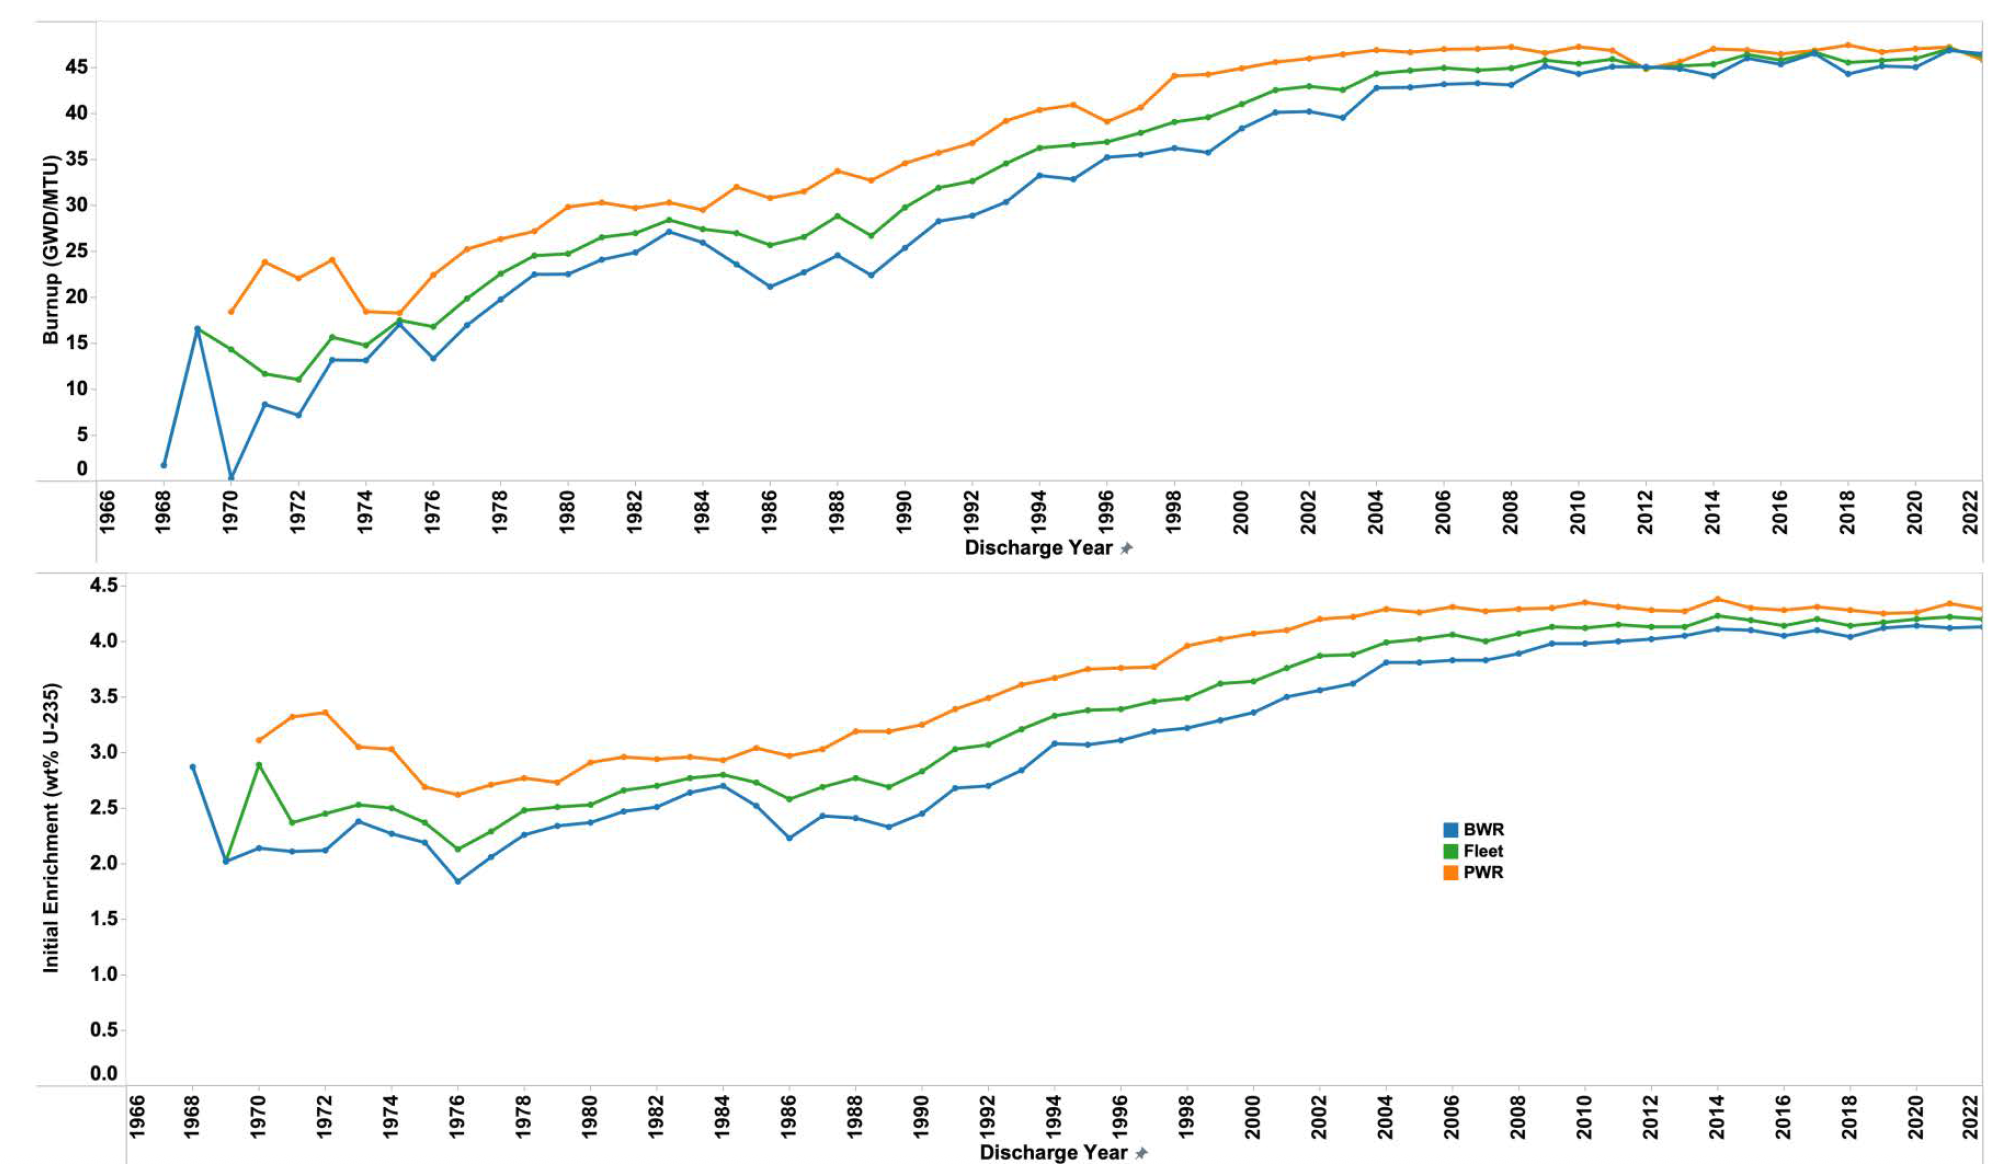
\includegraphics[width=\textwidth]
        {figures/burnup_enrichment.png}
    \caption{The annual average discharge burnup and initial
    \ce{^{235}U} enrichment of U.S. light water reactor fuel increased
    substantially between 1968 and 2022. Figure reproduced from \cite{carter_banerjee_inventory_2024}.}
    \label{fig:annual-burnup-enrichment}
\end{figure}


Figure~\ref{fig:assembly-burnup-enrichment} provides the corresponding
joint distribution of assembly burnup and initial enrichment in the inventory,
showing both the central concentration of the data and the smaller number of
assemblies at the extremes of the operating range.

\begin{figure}[htbp]
    \centering
    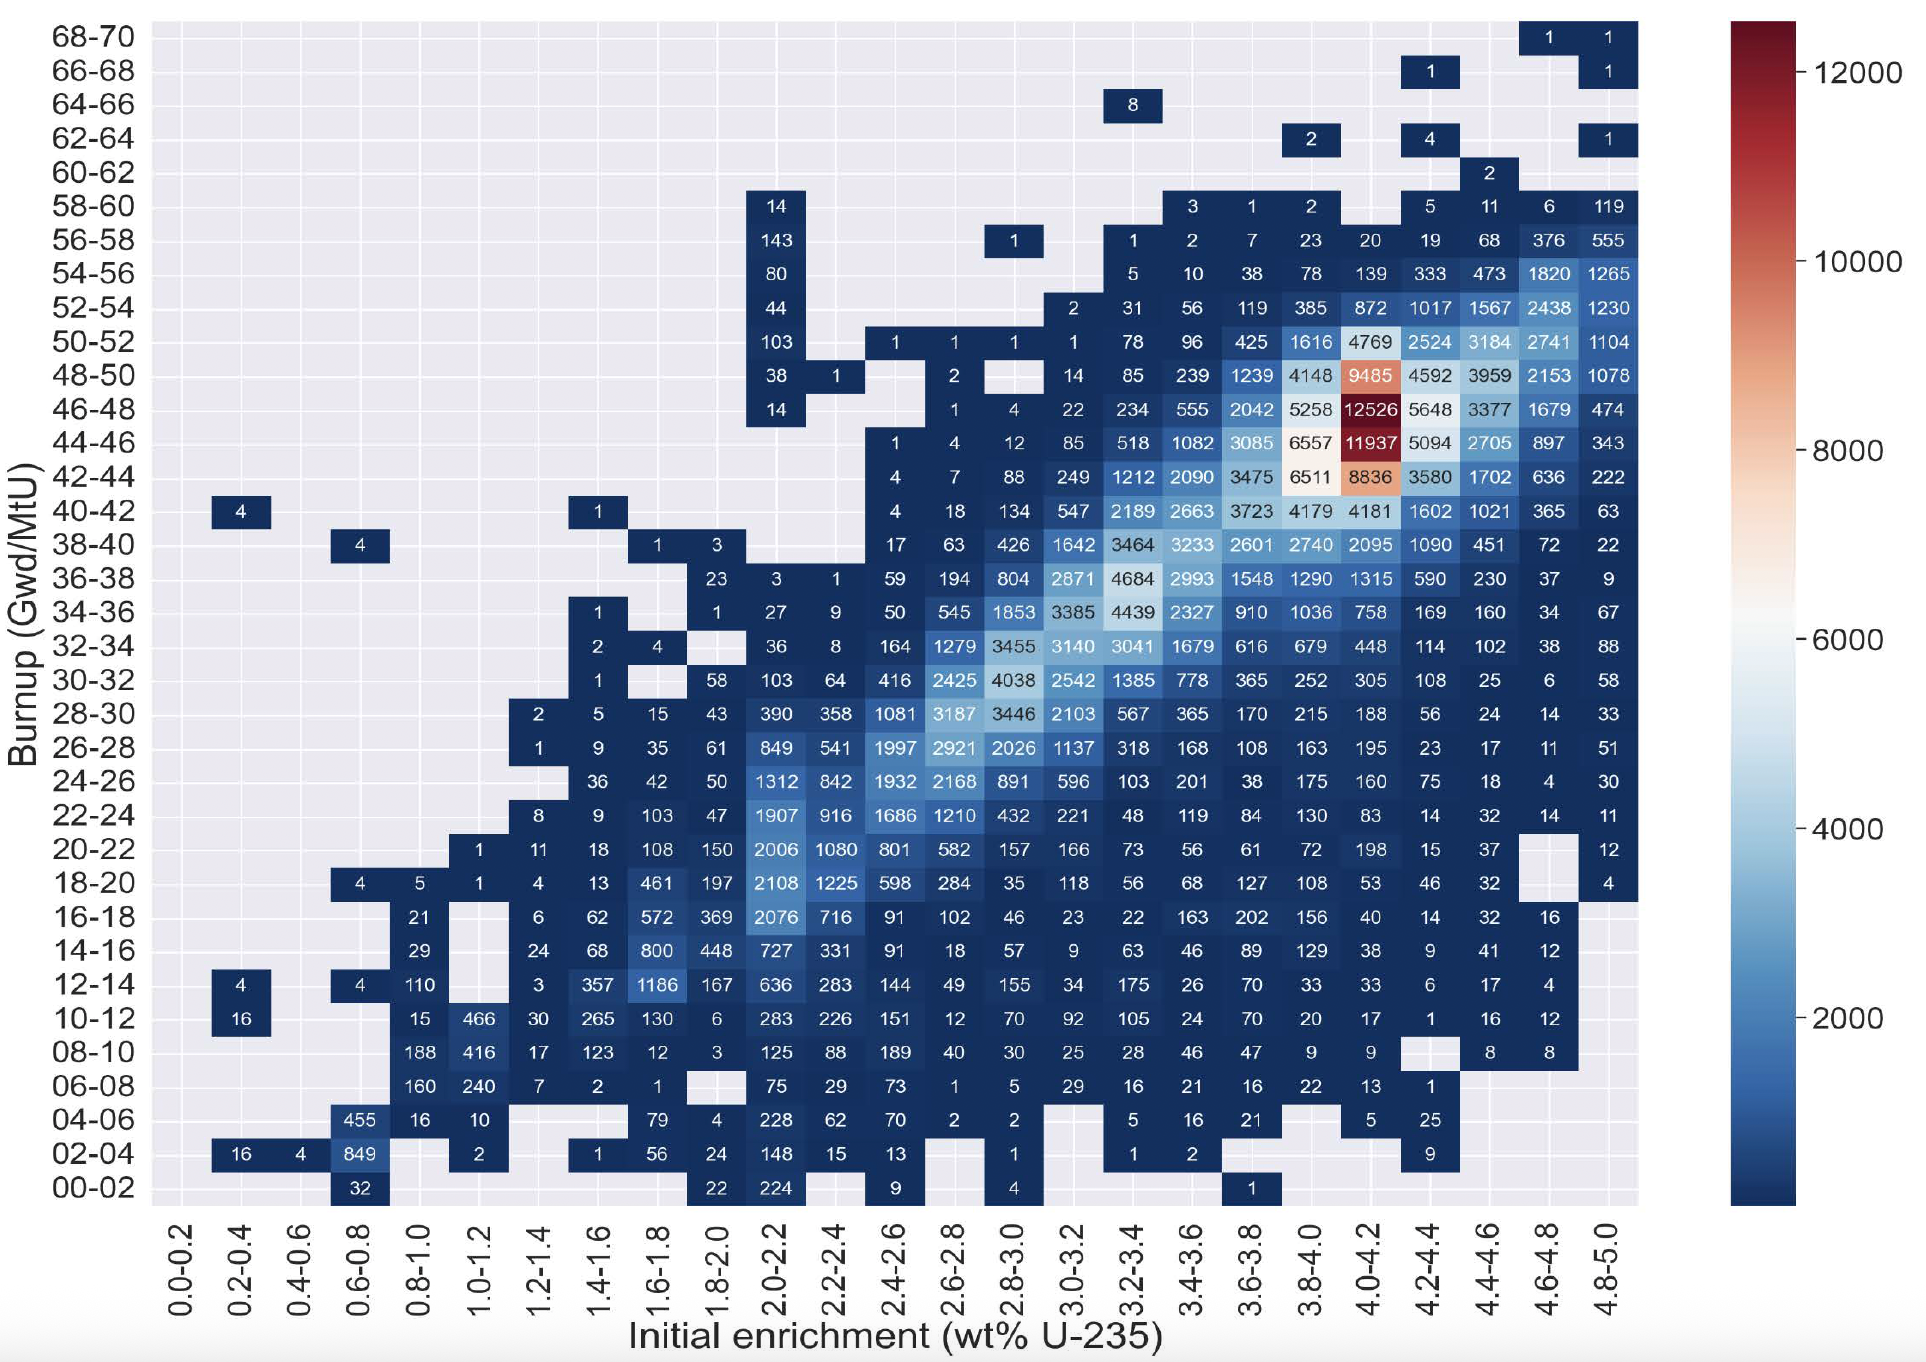
\includegraphics[width=\textwidth]{figures/assemblies.png}
    \caption{Burnup (GWd/MTHM) and initial enrichment (\% $^{235}U$)
    distributions for spent nuclear fuel assemblies in the \glspl{LWR}
    inventory through December 2022. Figure reproduced from
    \cite{carter_banerjee_inventory_2024}.}
    \label{fig:assembly-burnup-enrichment}
\end{figure}

Higher burnup changes the isotopic composition of discharged fuel. During
irradiation, neutron capture in \ce{^{238}U} produces plutonium isotopes, while
successive neutron capture and decay reactions generate neptunium, americium,
and curium. Extending irradiation therefore generally increases the production
of plutonium and minor actinides within an assembly, although the exact
inventory depends on enrichment, reactor type, neutron spectrum, power
history, and cooling time. The modern \gls{UNF} inventory is consequently not
uniform: assemblies discharged in different decades contain different
quantities of fissile material, transuranic elements, fission products, and
decay heat\cite{carter_banerjee_inventory_2024}.

These compositional differences are important because the nuclides that
control \gls{UNF} behavior change with cooling time. Shortly after discharge,
fission products dominate decay heat. In particular, \ce{^{137}Cs} and
\ce{^{90}Sr}, together with their decay products, are major contributors over
the first several decades. Their heat output decreases substantially as they
decay. Over longer periods, transuranic isotopes, especially plutonium and
americium isotopes, become the dominant contributors to the remaining heat
and radiotoxicity
\cite{carter_banerjee_inventory_2024}.

This transition is significant for the U.S. waste management strategy. Storage can
allow short-lived fission products to decay, but short-term storage does not eliminate
the fundamental long-term burden posed by plutonium and the minor actinides.
In a once-through fuel cycle, these nuclides must otherwise remain isolated while they decay over much
longer timescales. Alternatively, actinides can be separated and irradiated in a
suitable neutron spectrum, where fission converts them into shorter-lived
fission products while releasing additional energy. Long-lived fission
products may also be candidates for specialized transmutation, but the
actinides are the principal component of \gls{UNF} that can be destroyed through
fission rather than managed solely by long-term storage and geologic
isolation\cite{iaea_ma_fuels_2009}.

The increasing mass, geographic dispersion, and transuranic content of the
U.S. \gls{UNF} inventory therefore motivate the fuel cycle simulations in this
work. A realistic assessment of accelerator-driven transmutation must
represent not only the total mass of available fuel, but also the differences
among assemblies in discharge date, burnup, enrichment, location, and
isotopic composition. These attributes determine which portions of the
inventory can be selected, separated, and supplied to an accelerator-driven
system.

%%%%%%%%%%%%%%%%%%%%%%%%%%%%%%%%%%%%%%%%%%%%%%%%%%%%%%%%%%%%%%%%%%%%%%%%%%%%%%%%%%%%%%%%%%%%%%%%%%%%%%%%%%%%%%%%%%%%%%%%%%%%%%%%%%
%%%%%%%%%%%%%%%%%%%%%%%%%%%%%%%%%%%%%%%%%%%%%%%%%%%%%%%%%%%%%%%%%%%%%%%%%%%%%%%%%%%%%%%%%%%%%%%%%%%%%%%%%%%%%%%%%%%%%%%%%%%%%%%%%%%
%%%%%%%%%%%%%%%%%%%%%%%%%%%%%%%%%%%%%%%%%%%%%%%%%%%%%%%%%%%%%%%%%%%%%%%%%%%%%%%%%%%%%%%%%%%%%%%%%%%%%%%%%%%%%%%%%%%%%%%%%%%%%%%%
\section{The Cyclus Fuel Cycle Simulation Framework}
\label{sec:cyclus}

The two archetypes developed in this thesis are implemented within \Cyclus,
and their behavior can only be understood in relation to the framework's
underlying model of facilities, materials, and exchange. This section reviews
the aspects of \Cyclus most relevant to that implementation and introduces the agent-based
structure of the framework and how it represents fuel cycle facilities and
their interactions over time. Then moving on to describe how materials and their
isotopic compositions are represented and how radioactive decay is applied,
which is central to tracking the evolving minor actinide vector on which this
work depends and explains the \gls{DRE}, the mechanism through
which facilities request, offer, and trade resources at each time step.

\subsection{Framework Basics}
\label{subsec:cyclus-framework-basics}

\Cyclus is an open-source, agent-based nuclear fuel cycle simulation
framework designed to represent the deployment, operation, and interaction
of nuclear fuel cycle facilities over time. The framework tracks discrete
facilities and material resources rather than representing the fuel cycle
solely through aggregated fleet-level flows. This design supports analyses
in which individual facility behavior, material availability, and institutional
decisions influence system level outcomes
\cite{huff_fundamental_2016}.

Agents in a \Cyclus simulation are organized into three hierarchical types:
regions, institutions, and facilities. Regions form the highest organizational
level and may represent countries, geographic areas, or other broad
groupings. Institutions operate within regions and manage the deployment
and retirement of facilities. Facilities represent physical or functional
components of the nuclear fuel cycle, including mines, enrichment plants,
reactors, separations facilities, storage facilities, and repositories
\cite{huff_fundamental_2016}.

A \Cyclus simulation advances through discrete time steps, commonly
defined as months. During each time step, facilities may request resources,
offer available resources, conduct material transactions, process their
inventories, and update their internal states. Modeling facilities and time
discretely allows the framework to capture effects such as asynchronous
reactor refueling, temporary shortages of fuel cycle materials, and 
differences in facility deployment and retirement schedules\cite{gidden_agent-based_2015}.

The behavior of each agent is defined by an \emph{archetype}. Archetypes
are modular software components that implement the physical behavior,
operating logic, or decision rules of a region, institution, or facility.
They are compiled independently from the \Cyclus kernel and loaded
dynamically at the beginning of a simulation. This plug in architecture
allows alternative models of the same fuel cycle process to be exchanged
without modifying the core simulation framework
\cite{huff_fundamental_2016,scopatz_cyclus_2015}.

The \Cyclus kernel provides shared simulation services, including time
management, agent deployment, resource tracking, data recording, and
resource exchange. Archetypes access these services through the agent
application programming interface. As illustrated in
Figure~\ref{fig:cyclus-architecture}, the kernel provides the central
simulation environment, the agent interface connects the kernel to agent
models, and independently developed archetype libraries provide the
behavior of the simulated regions, institutions, and facilities.

\begin{figure}[htbp]
    \centering
    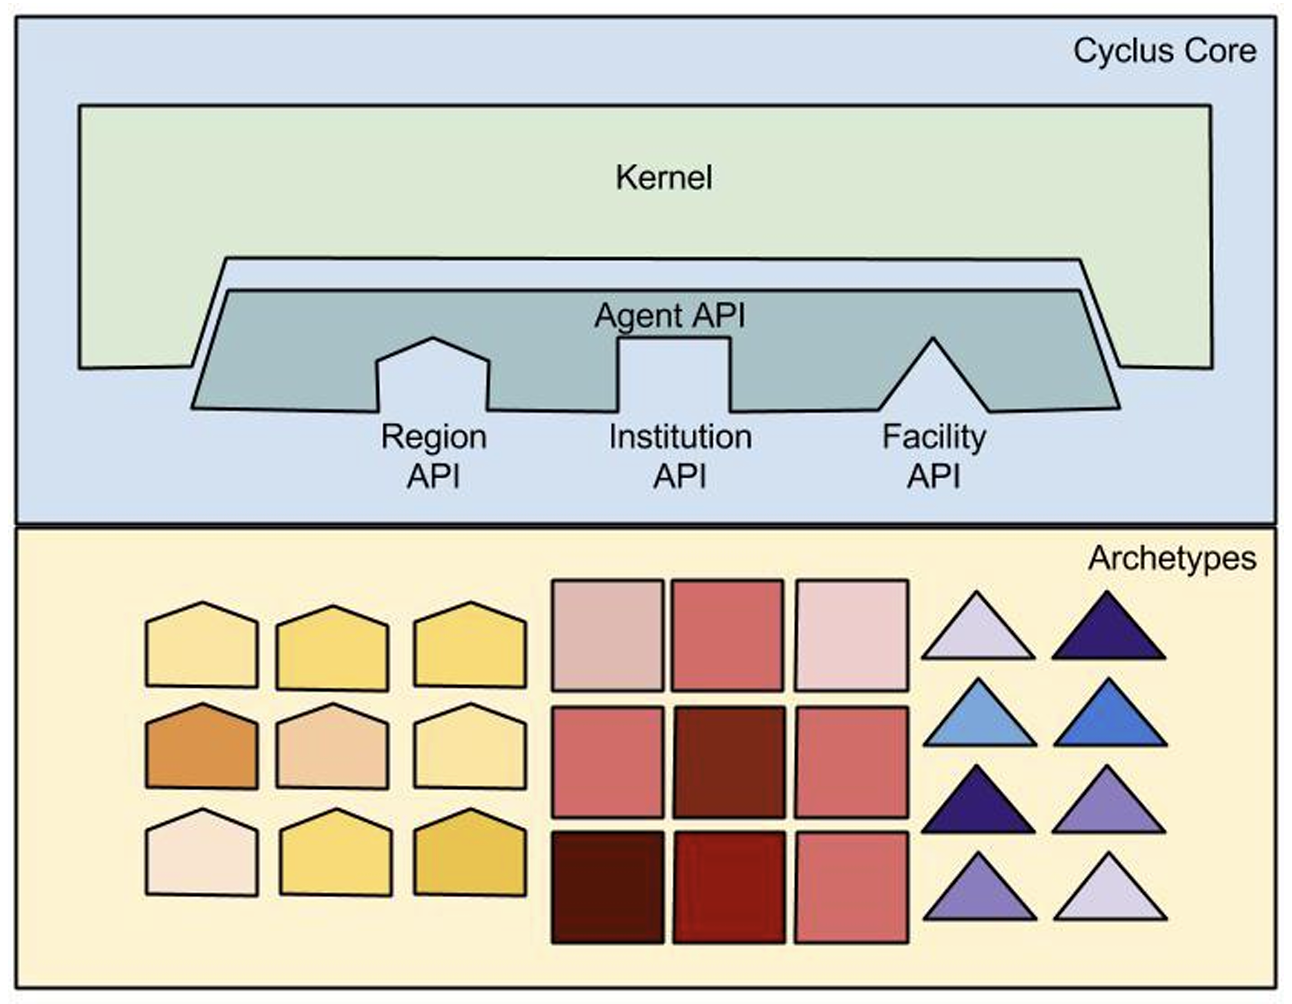
\includegraphics[width=0.75\textwidth]
        {figures/Cyclus.png}
    \caption{The \Cyclus simulation architecture separates the core kernel
    from dynamically loaded region, institution, and facility archetypes
    through the Agent \gls{API}. Figure reproduced from \cite{huff_fundamental_2016}.}
    \label{fig:cyclus-architecture}
\end{figure}


\subsection{Materials and Decay}
\label{subsec:cyclus-materials-decay}


Resources exchanged in \Cyclus are represented as discrete objects. The two
primary resource types are \emph{materials} and \emph{products}. A material
resource has an associated quantity and isotopic composition, whereas a
product represents a non-nuclear resource whose quality may be described
without a nuclide vector. Nuclear fuel cycle simulations therefore generally
use material resources to represent fresh fuel, spent nuclear fuel, separated
actinides, and radioactive waste \cite{huff_fundamental_2016}.

A \Cyclus material object contains a total mass and a \emph{Composition}
object. The composition stores the relative abundance of the nuclides present
in the material and is treated independently from the material quantity.
This separation allows multiple material objects to reference the same
composition and permits operations such as splitting, combining, and
transmuting material while preserving mass accounting. Materials may also
be stored in facility inventories and exchanged between agents through the
resource exchange system.

Radioactive decay can be applied directly to material resources within
\Cyclus. When a material is decayed over a specified time interval, its
nuclide vector is updated according to the radioactive decay chains available
to the framework. The decay calculation uses nuclear data supplied through
PyNE \cite{scopatzPyNEPythonNuclear2012}, which is an open-source nuclear engineering toolkit
that supplies the nuclear data including half-lives, decay constants, branching relationships, and
daughter products. The total quantity of a material remains associated with
the resource while its isotopic composition changes with time
\cite{huff_fundamental_2016}.

Decay in the simulations developed for this work is handled at the
simulation level through the \Cyclus control block, with decay set to
\texttt{lazy}. Under this setting the kernel decays a material's composition
on demand rather than at every time step, computing the decayed nuclide
vector when a composition is next inspected and caching the result for reuse
\cite{huff_fundamental_2016}. This choice retains the physical effect of
radioactive decay over the multi-decade simulation horizon while avoiding
the cost of decaying every inventory at every step. Decay is significant
over this horizon: the roughly 14-year half-life of \ce{^{241}Pu}, for
example, produces appreciable ingrowth of \ce{^{241}Am} across a
thirty-year run, altering the minor actinide vector that the inventory and
accelerator-driven system models are designed to track.


\subsection{The Dynamic Resource Exchange}
\label{subsec:cyclus-dre}

Transactions among \Cyclus facilities are coordinated through the \gls{DRE}. The \gls{DRE} provides a general
mechanism through which independently developed archetypes can exchange
resources without requiring direct knowledge of one another's internal
implementation. Facilities communicate their demand and supply to the
framework, and the exchange system determines a feasible set of transactions
for each time step \cite{huff_fundamental_2016}.

The exchange begins when consuming facilities generate requests for
resources. A request identifies a desired commodity, quantity, and, when
relevant, a target material composition or other resource quality. Supplying
facilities evaluate these requests and generate bids describing the resources
they are able to provide. A bid links a particular offered resource to a
request and may provide all or only part of the requested quantity\cite{gidden_agent-based_2015}.

Facilities may also assign preferences to possible trading partners or
resources. Preferences allow a requester to rank otherwise feasible bids,
for example by favoring a particular supplier, fuel composition, or material
characteristic. In addition, suppliers and requesters may impose constraints
such as production capacity, inventory availability, throughput, or minimum
and maximum transaction quantities. These constraints define which
combinations of trades are physically or operationally feasible.

The requests, bids, preferences, and constraints form a resource assignment
problem. \Cyclus formulates this assignment as an optimization problem, solvable in
either a linear or a mixed-integer form, and the \gls{DRE} solves it to select a
set of transactions that satisfies the applicable constraints while favoring
higher preference trades \cite{gidden_agent-based_2015}.
After the solution is determined, the participating facilities execute the
selected transactions and update their inventories. This process is repeated
at each simulation time step, allowing supply and demand relationships to
change dynamically as facilities are deployed, retired, depleted, or otherwise
alter their behavior.

By separating exchange coordination from facility specific behavior, the \gls{DRE}
allows archetypes to be developed and combined modularly. A storage facility,
reactor, separations plant, or repository can participate in the same exchange
system as long as it implements the appropriate request, bidding, and trade
interfaces. This separation is particularly important for this work because
the inventory and accelerator-driven system models must interact with both
existing and newly developed fuel cycle facilities.

\subsection{Extensions Developed in This Work}
\label{subsec:cyclus-extensions}

This work extends the \Cyclus ecosystem and its \texttt{cycamore} archetype library
\cite{carlsen_cycamore_2014} with two facility archetypes developed
within the \texttt{einstein} archetype library. The \texttt{us\_inventory}
facility represents the U.S. spent nuclear fuel inventory at assembly
resolution, reading isotopic compositions and assembly metadata from the
\gls{STANDARDS}~5.0.1 dataset\cite{peterson_unf-st&dards_2017,peterson_additional_2017}
and supplying material according to user-selected inventory selection policies.
The \texttt{ads} facility represents an accelerator-driven subcritical burner, transforming a
loaded core composition using a library of precomputed Serpent depletion
cases. Both archetypes participate in the resource exchange described above:
\texttt{us\_inventory} as a supplier whose selection policies determine which
assemblies it offers against a given request, and \texttt{ads} as a requester
whose feed preferences rank inventory and separations output. Their design,
implementation, and the four simulation scenarios in which they are exercised
are described in Chapter~\ref{ch:methodology}.


%%%%%%%%%%%%%%%%%%%%%%%%%%%%%%%%%%%%%%%%%%%%%%%%%%%%%%%%%%%%%%%%%%%%%%%%%%%%%%%%%%%%%%%%%%%%%%%%%%%%%%%%%%%%%%%%%%%%%%%%%%%%%%%%%%
%%%%%%%%%%%%%%%%%%%%%%%%%%%%%%%%%%%%%%%%%%%%%%%%%%%%%%%%%%%%%%%%%%%%%%%%%%%%%%%%%%%%%%%%%%%%%%%%%%%%%%%%%%%%%%%%%%%%%%%%%%%%%%%%%%%
%%%%%%%%%%%%%%%%%%%%%%%%%%%%%%%%%%%%%%%%%%%%%%%%%%%%%%%%%%%%%%%%%%%%%%%%%%%%%%%%%%%%%%%%%%%%%%%%%%%%%%%%%%%%%%%%%%%%%%%%%%%%%%%%

\section{Accelerator-Driven Systems}
\label{sec:ads}

\glspl{ADS} combine a high-power particle accelerator
with a subcritical nuclear assembly. They have been proposed as dedicated
systems for the transmutation of plutonium, minor actinides, and selected
long-lived fission products recovered from spent nuclear fuel
\cite{iaea_ma_fuels_2009}.
The \gls{ADS} concept is particularly relevant to this work because it provides a
potential pathway for consuming materials that is rich in minor actinides that present
significant neutronic and safety challenges in critical reactors.

\subsection{System Components and Operation}
\label{subsec:ads-components}

An \gls{ADS} consists of three principal components: a high-energy proton
accelerator, a spallation target, and a subcritical multiplying core. The
accelerator produces a proton beam, often with an energy of several hundred
megaelectronvolts to approximately one gigaelectronvolt. The beam strikes a
heavy metal target, where high energy proton-nucleus interactions release
neutrons through the spallation process. These source neutrons enter the
surrounding subcritical core and induce fission reactions in the fuel
\cite{aitabderrahim_myrrha_2001,nea_ads_components_2010}.

The target must generate a sufficiently intense neutron source while
withstanding substantial beam heating, radiation damage, and mechanical
loading. Heavy elements are attractive target materials because they produce
relatively large numbers of neutrons when bombarded by high-energy protons.
Proposed \gls{ADS} targets include solid tungsten targets and liquid metal targets
based on lead or lead-bismuth eutectic. In some designs, a circulating
liquid metal target also contributes to heat removal
\cite{aitabderrahim_myrrha_2001,nea_ads_components_2010}.

The core is designed to remain subcritical, such that

\begin{equation}
    k_{\mathrm{eff}} < 1,
\end{equation}

where \(k_{\mathrm{eff}}\) is the effective neutron multiplication factor.
Unlike a critical reactor, the neutron population in an \gls{ADS} core cannot
sustain itself indefinitely without the external spallation source. Source
neutrons initiate fission reactions and are multiplied within the subcritical
core, allowing the thermal power produced by fission to exceed the power
delivered by the proton beam
\cite{eriksson_ads_safety_2004,nea_ads_components_2010}.

The accelerator therefore provides an additional mechanism for controlling
the fission power. When the beam is interrupted, the external source of
spallation neutrons is removed and the source-driven fission power decreases
rapidly. This behavior is sometimes described by stating that the beam acts
as an on-off switch for the fission chain. However, turning off the beam
does not eliminate radioactive decay heat. The fuel and structures continue
to generate heat after shutdown and require reliable residual heat removal
\cite{eriksson_ads_safety_2004}.

Figure~\ref{fig:ads-components} illustrates the relationship among the
accelerator, spallation target, and subcritical core.

\begin{figure}[htbp]
    \centering
    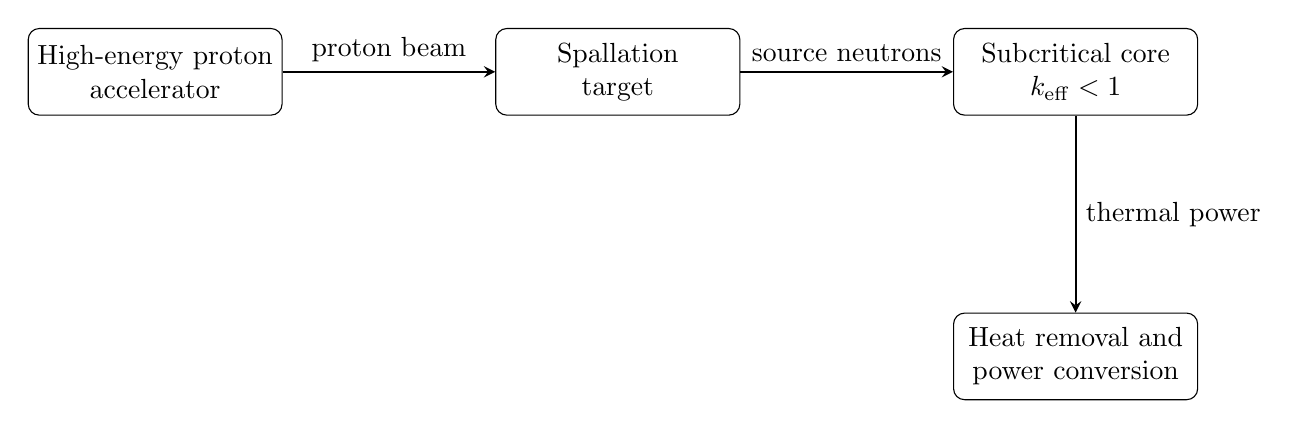
\begin{tikzpicture}[
        node distance=2.5cm and 2.7cm,
        component/.style={
            rectangle,
            rounded corners,
            draw=black,
            minimum width=3.1cm,
            minimum height=1.1cm,
            align=center
        },
        flow/.style={thick,->,>=stealth}
    ]

    \node[component] (accelerator)
        {High-energy proton\\accelerator};

    \node[component, right=of accelerator] (target)
        {Spallation\\target};

    \node[component, right=of target] (core)
        {Subcritical core\\\(k_{\mathrm{eff}} < 1\)};

    \node[component, below=of core] (heat)
        {Heat removal and\\power conversion};

    \draw[flow]
        (accelerator) --
        node[above]{proton beam}
        (target);

    \draw[flow]
        (target) --
        node[above]{source neutrons}
        (core);

    \draw[flow]
        (core) --
        node[right]{thermal power}
        (heat);

    \end{tikzpicture}

    \caption{Principal components and energy flows of an
    accelerator-driven subcritical system. This original schematic is based
    on the \gls{ADS} descriptions presented in
    \cite{aitabderrahim_myrrha_2001,nea_ads_components_2010}.}
    \label{fig:ads-components}
\end{figure}

Accelerator-driven transmutation of used nuclear fuel received sustained
attention in the United States during the late 1990s and early 2000s, most
prominently through the \gls{ATW} program,
which developed system scenarios and integration roadmaps for dedicated
subcritical burners \cite{vantuyleRoadmapDevelopingATW2001}. Interest in the approach has
since reemerged in the context of managing the growing national
inventory.

\subsection{Minor Actinide Transmutation}
\label{subsec:ads-ma-transmutation}

The principal motivation for using \gls{ADS} technology for nuclear waste
management is its ability to accommodate fuels containing large fractions of
minor actinides. The minor actinides most commonly considered for
transmutation are neptunium, americium, and curium. These nuclides contribute
to the long-term radiotoxicity and decay heat of spent nuclear fuel. Their
separation and irradiation in a dedicated transmutation system could reduce
the quantity of long-lived transuranic material requiring disposal
\cite{iaea_ma_fuels_2009}.

Fast neutron spectra are generally preferred for minor actinide
transmutation because fission becomes more competitive with radiative
capture for many transuranic isotopes at higher neutron energies. A
fast spectrum system can therefore destroy minor actinides through fission
rather than merely converting them into heavier actinides
\cite{iaea_ma_fuels_2009}.

However, loading a critical fast reactor with a high concentration of minor
actinides introduces important safety and control challenges. Fuel rich in minor actinides
generally has a smaller effective delayed neutron fraction than
conventional uranium- or plutonium-bearing fuel. Although delayed neutrons
represent only a small fraction of the total fission neutron population, they
substantially slow the response of a critical reactor to reactivity changes.
A reduction in the effective delayed neutron fraction therefore causes the
reactor power to respond more rapidly to disturbances
\cite{eriksson_ads_safety_2004}.

Minor actinide loading may also reduce the magnitude of negative Doppler
reactivity feedback. In conventional reactor fuel, increasing fuel
temperature broadens neutron absorption resonances and generally introduces
negative reactivity. This prompt feedback opposes the temperature increase.
The magnitude of this effect can be weaker in minor actinide rich,
fast spectrum fuels because of their isotopic composition and the reduced
importance of resonance absorption in a fast spectrum
\cite{eriksson_ads_safety_2004,iaea_ma_fuels_2009}.

The combination of a reduced delayed neutron fraction and weaker negative
Doppler feedback makes a critical core with a high minor actinide content
more difficult to control. Critical fast reactor concepts may therefore limit
the amount of minor actinides loaded in the core or distribute them among
fuel containing larger quantities of uranium or plutonium\cite{eriksson_ads_safety_2004}.

Subcritical operation provides an alternative approach. Because the core
remains below criticality and relies on an external neutron source, an \gls{ADS}
can accommodate fuel compositions that would be difficult to use at high
concentrations in a critical reactor. Subcriticality provides additional
margin against prompt criticality and separates, to some extent, the control
of the neutron source from the inherent reactivity of the fuel
\cite{eriksson_ads_safety_2004}.

Subcriticality does not eliminate the need to evaluate reactivity accidents,
cooling failures, material behavior, or decay heat removal. Nevertheless, it
relaxes an important neutronic constraint on the amount of minor actinides
that can be loaded into a dedicated transmutation system. This capability is
the central reason that \gls{ADS} technology is relevant to this thesis. The
purpose of the modeled fuel cycle is to connect separated material from the
U.S. spent nuclear fuel inventory with systems capable of consuming
minor actinider streams that may not be suitable for concentrated use in
critical reactors.

\subsection{Target and Coolant Options}
\label{subsec:ads-target-coolant}

\gls{ADS} concepts differ in their target materials, coolants, fuel forms, neutron
spectra, and power levels. Lead and lead-bismuth eutectic are among the
most frequently proposed heavy liquid metals because their large atomic
masses support spallation neutron production and their high boiling
temperatures permit low pressure primary systems
\cite{aitabderrahim_myrrha_2001,nea_ads_components_2010}.

Lead-bismuth eutectics can have a substantially lower melting temperature than
pure lead, reducing some of the operational challenges associated with
coolant freezing. The most advanced current example is \gls{MYRRHA}, a lead-bismuth-cooled
subcritical system under development at the Belgian Nuclear Research Centre.
Its first phase, the \gls{MINERVA} proton accelerator and target facility, began
construction in 2024 \cite{dordaImplementationStatusMyrrha2024}, making \gls{MYRRHA} the closest
existing demonstration of the accelerator driven concept.
However, neutron activation of bismuth produces
polonium-210, which creates radiological and maintenance concerns. Both
lead and lead-bismuth can also cause corrosion or erosion of structural
materials. Their use therefore requires careful control of coolant chemistry,
oxygen concentration, temperature, and flow conditions
\cite{nea_ads_components_2010}.

Pure lead avoids the production of polonium associated with bismuth but has
a higher melting temperature. This increases the importance of freeze
prevention during startup, shutdown, and off-normal operation. Despite this
challenge, lead has been proposed both as a coolant and as a carrier medium
for mobile fuel \gls{ADS} concepts\cite{nea_ads_components_2010,gohar_ads_2021}.

The \gls{ADS} concept that provides the initial technical basis for the \gls{EINSTEIN}
project was developed to transmute material derived from the U.S. spent
nuclear fuel inventory. The proposed system uses a high energy proton
accelerator, a spallation neutron source, and a lead-based subcritical system.
The fuel concept contains plutonium and minor actinides in a mobile
lead-based medium, permitting continuous or periodic processing of the fuel
inventory \cite{gohar_ads_2021}.

Gas cooled \gls{ADS} concepts have also been investigated. Helium is chemically
inert and avoids many of the corrosion and activation issues associated with
heavy liquid metals. However, its low density and volumetric heat capacity
require high pressure operation and significant pumping power. The coolant
and target selection therefore influences neutron production, material
compatibility, plant efficiency, operating pressure, safety behavior, and
the design of the primary heat removal system
\cite{nea_ads_components_2010}.

\subsection{Technical and Economic Limitations}
\label{subsec:ads-limitations}

Despite their potential advantages for transmutation, \gls{ADS} facilities face
substantial technical and economic challenges. Accelerator availability is
one of the most important engineering concerns. A sudden beam interruption
causes a rapid decrease in fission power and temperature. Restoration of the
beam causes the power and temperature to increase again. Repeated beam
interruptions can therefore impose cyclic thermal loads on the fuel,
spallation target, coolant systems, and structural components
\cite{nea_beam_interruptions_2004}.

The \gls{OECD} Nuclear Energy Agency beam interruption benchmark specifically
examined the temperature transients caused by beam trips in a
lead-bismuth-cooled, subcritical system. The study identified thermal
fatigue of structural components as an important consequence of repeated
beam interruptions \cite{nea_beam_interruptions_2004}. More recent analysis
of the China Initiative Accelerator Driven System has also evaluated fuel
cladding fatigue under repeated beam trip transients
\cite{wang_beam_trips_2024}.

Producing a continuous, high-current proton beam with the availability
required for a power producing nuclear system is more demanding than
operating an accelerator intended for intermittent research use.
Fault-tolerant accelerator designs, redundant components, and rapid recovery
procedures may reduce the number and duration of beam interruptions, but
these features add complexity and cost
\cite{nea_ads_components_2010}.

The spallation target presents additional engineering challenges. It must
tolerate concentrated beam heating, radiation damage, gas production,
thermal stresses, and interactions with the coolant. Target replacement,
inspection, and maintenance must also be performed in a highly radioactive
environment \cite{nea_ads_components_2010}.

\gls{ADS} deployment additionally requires supporting fuel cycle infrastructure.
Spent nuclear fuel must first be processed to recover the actinides intended
for transmutation. The resulting material rich in minor actinides must then be
fabricated into fuel or introduced into an appropriate mobile fuel medium.
After irradiation, the material may require repeated separation and recycle
to achieve substantial actinide destruction. These activities introduce
material losses, secondary waste streams, safeguards requirements, worker
exposure, and additional facilities\cite{iaea_ma_fuels_2009}.

An \gls{ADS} also combines the capital cost and regulatory requirements of a
nuclear reactor facility with those of a high-power accelerator. Furthermore,
the accelerator consumes a portion of the electricity generated by the
system. Comparative \gls{OECD}/\gls{NEA} studies have therefore emphasized that the
potential transmutation benefits of \gls{ADS} technology must be evaluated
alongside its fuel cycle requirements, technical complexity, research and
development needs, and economic performance\cite{eriksson_ads_safety_2004}.

These limitations make a system level fuel cycle analysis necessary. The
performance of an \gls{ADS} cannot be judged solely from the rate of transmutation
inside its core. A complete assessment must also consider the availability
and composition of feed material, separations capacity, facility deployment,
accelerator and reactor throughput, recycle requirements, and the production
of secondary waste streams. These interactions motivate the \Cyclus
simulation models developed in this work.


%%%%%%%%%%%%%%%%%%%%%%%%%%%%%%%%%%%%%%%%%%%%%%%%%%%%%%%%%%%%%%%%%%%%%%%%%%%%%%%%%%%%%%%%%%%%%%%%%%%%%%%%%%%%%%%%%%%%%%%%%%%%%%%%%%
%%%%%%%%%%%%%%%%%%%%%%%%%%%%%%%%%%%%%%%%%%%%%%%%%%%%%%%%%%%%%%%%%%%%%%%%%%%%%%%%%%%%%%%%%%%%%%%%%%%%%%%%%%%%%%%%%%%%%%%%%%%%%%%%%%%
%%%%%%%%%%%%%%%%%%%%%%%%%%%%%%%%%%%%%%%%%%%%%%%%%%%%%%%%%%%%%%%%%%%%%%%%%%%%%%%%%%%%%%%%%%%%%%%%%%%%%%%%%%%%%%%%%%%%%%%%%%%%%%%%

\section{The EINSTEIN Program}
\label{sec:einstein}

The Enhanced Integrated Nuclear Systems for Transmutation and Efficient Isolation of Nuclides (\gls{EINSTEIN})
project is part of the \gls{ARPAE} Nuclear Energy Waste Transmutation Optimized Now (\gls{NEWTON}) program.
The \gls{NEWTON} program was established to support
technologies that enable the transmutation of used nuclear fuel and reduce
the burden placed on permanent waste disposal facilities
\cite{arpa_e_newton_2025}. The \gls{EINSTEIN} project is led by the University of Illinois Urbana-Champaign
\cite{arpa_e_einstein_2025}.

\gls{NEWTON} addresses the transmutation problem through three complementary
technical categories. Category A focuses on technologies for generating and
accelerating particle beams capable of initiating transmutation reactions.
Category B focuses on the design, fabrication, and processing of targets or
fuel forms containing the nuclides to be transmuted. Category C integrates
the technologies developed in Categories A and B through system level
modeling, life cycle analysis, techno-economic analysis, and databases of
materials and components
\cite{arpa_e_newton_2025,doe_categories}. \gls{UIUC} is a Category C and therefore
does not develop a single accelerator or transmutation target in isolation.
Instead, it provides a common framework for comparing candidate systems and
identifying the technical and economic conditions under which they could
contribute to management of the U.S. used nuclear fuel inventory.

Within the \gls{EINSTEIN} project, the term \acrshort{XDS} refers collectively
to subcritical transmutation systems sustained by an external neutron source.
Within this framing, \glspl{ADS} use an accelerator and spallation target to
produce the source neutrons, while \glspl{FDS} use neutrons generated by a
fusion source. The two classes may differ substantially in neutron energy,
source geometry, target and coolant materials, reliability constraints, and
technology readiness. Nevertheless, both couple an external neutron source to
a subcritical multiplying region and can therefore be represented within a
common fuel cycle and assessment framework. The initial \gls{EINSTEIN} analyses
include a high-energy, proton-driven, lead-cooled \gls{ADS} and a
\(14.1~\mathrm{MeV}\) fusion-neutron-driven, salt-cooled system
\cite{fang_einstein_2025}.

The central objective of \gls{EINSTEIN} is to develop a data-informed framework for
rapidly assessing \gls{XDS} technologies according to both their transmutation
performance and their financial implications. The project connects nuclear
data, neutronics, materials compatibility, fuel cycle behavior, and economic
performance rather than evaluating each component independently. The
official project description identifies the development of a comprehensive
life cycle analysis framework spanning the full transmutation process, from
the composition of the incoming used fuel stream through irradiation,
processing, and the resulting waste or product streams
\cite{arpa_e_einstein_2025}. Experimental and computational activities are
used to reduce uncertainties in neutron transport, material properties, and
component performance.

The \gls{UIUC} project team is organized around several interacting technical
areas as shown in Figure~\ref{fig:uiuc-einstein}. Nuclear data and diagnostics work identifies reactions whose
uncertainties significantly affect neutron multiplication and transmutation
predictions and develops experimental strategies to reduce those
uncertainties. Neutronics analysis provides source term, criticality,
depletion, and transmutation calculations for selected \gls{XDS} concepts.
Materials research evaluates corrosion, irradiation damage, thermophysical
properties, and the chemical behavior of lead coolants and molten salts.
Experimental work investigates the stability and solubility of representative
actinide surrogates and the compatibility of structural materials with the
candidate coolant and fuel media
\cite{fang_einstein_2025}.

\begin{figure}[htbp]
    \centering
    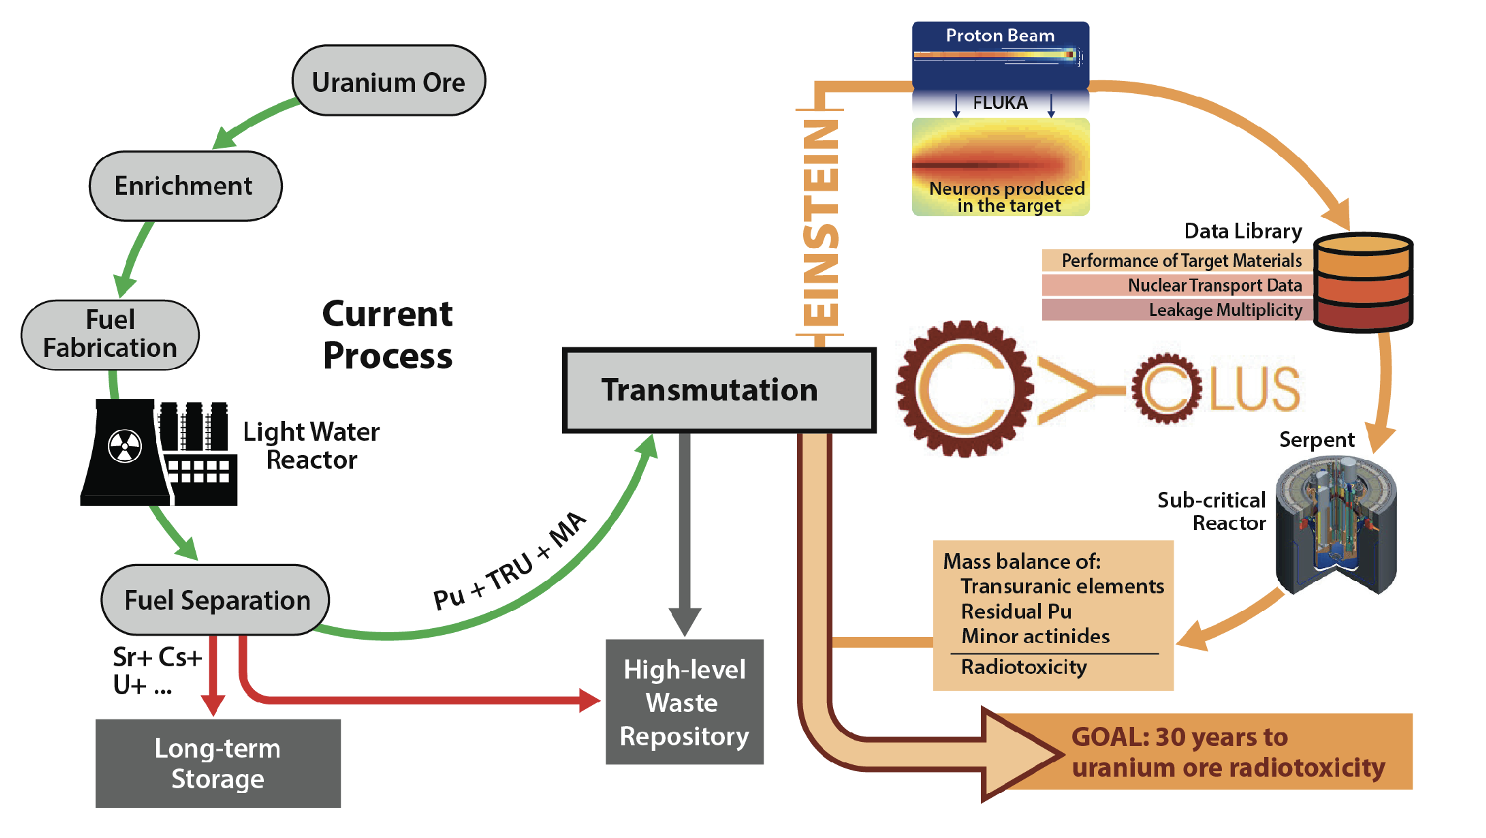
\includegraphics[width=\textwidth]
        {figures/EINSTEIN}
    \caption{Overview of the UIUC EINSTEIN project, which integrates FLUKA,
Serpent, nuclear data, materials, and \Cyclus fuel cycle analyses to evaluate
accelerator-driven transmutation of plutonium and minor actinides from used
nuclear fuel. The project aims to reduce the radiotoxicity of the remaining
waste to approximately that of natural uranium ore within 30 years. Figure reproduced from \cite{fang_einstein_2025}.}
    \label{fig:uiuc-einstein}
\end{figure}


These activities supply the inputs required for the fuel cycle and
techno-economic assessment. The fuel cycle portion of the project represents
the U.S. used nuclear fuel inventory, separations facilities, \gls{XDS} facilities,
recycle pathways, storage facilities, and waste streams in \Cyclus. The
inventory characterization begins with national spent fuel records and
age-corrected isotopic compositions, which are used to define realistic feed
streams for the modeled \gls{XDS} technologies. New \Cyclus archetypes are then
used to evaluate how the choice of feed material, facility throughput,
deployment schedule, separations capacity, and material selection policy
affects system level transmutation performance
\cite{fang_einstein_2025}.

The techno-economic analysis uses the outputs of the fuel cycle and
component models to examine capital costs, operating costs, potential
revenues, return on investment, and the sensitivity of economic conclusions
to uncertain design parameters. This coupling is important because a design
that performs well in a stand-alone neutronics calculation may still require
an impractical number of facilities, excessive separations capacity, costly
transportation, or unavailable supporting infrastructure. Conversely, a
concept with a lower per-facility transmutation rate may be more attractive
if it is easier to deploy, operate, and integrate with the existing nuclear
fuel cycle.

The work presented in this thesis lies primarily within the fuel cycle
modeling portion of \gls{EINSTEIN}. It develops the \texttt{us\_inventory} and
\texttt{ads} archetypes in the \texttt{einstein} library and uses them to
connect the characteristics of the national used fuel inventory with
candidate \gls{XDS} deployment scenarios. The resulting simulations provide
material flow, facility scaling, and inventory depletion information that can
be combined with the neutronics, materials, and economic analyses performed
elsewhere in the project. In this way, the thesis contributes the system level
link between the physical design of an \gls{XDS} and its potential effect on the
U.S. used nuclear fuel inventory.


%%%%%%%%%%%%%%%%%%%%%%%%%%%%%%%%%%%%%%%%%%%%%%%%%%%%%%%%%%%%%%%%%%%%%%%%%%%%%%%%%%%%%%%%%%%%%%%%%%%%%%%%%%%%%%%%%%%%%%%%%%%%%%%%%%
%%%%%%%%%%%%%%%%%%%%%%%%%%%%%%%%%%%%%%%%%%%%%%%%%%%%%%%%%%%%%%%%%%%%%%%%%%%%%%%%%%%%%%%%%%%%%%%%%%%%%%%%%%%%%%%%%%%%%%%%%%%%%%%%%%%
%%%%%%%%%%%%%%%%%%%%%%%%%%%%%%%%%%%%%%%%%%%%%%%%%%%%%%%%%%%%%%%%%%%%%%%%%%%%%%%%%%%%%%%%%%%%%%%%%%%%%%%%%%%%%%%%%%%%%%%%%%%%%%%%

\section{Prior Fuel Cycle Simulations of Transmutation Systems}
\label{sec:litrev}

Research on accelerator-driven transmutation has progressed through several
distinct stages. Early studies established the physics of coupling an intense
accelerator-produced neutron source to a subcritical multiplying medium.
Subsequent programs developed and tested individual enabling technologies,
including high current accelerators, liquid metal spallation targets,
subcriticality monitoring methods, minor actinide fuels, and lead or
lead-bismuth coolant systems. More recent studies have examined how dedicated
transmutation facilities could be incorporated into regional or national
nuclear fuel cycles.

These bodies of work do not all address the same modeling question. Reactor
physics studies generally evaluate neutron multiplication, power
distributions, safety coefficients, and nuclide destruction within one core.
Technology demonstrators test particular components or operating procedures.
Fuel cycle scenario studies instead examine the deployment of many reactors
and supporting facilities over several decades, tracking quantities such as
plutonium and minor actinide inventories, separations requirements, fuel
fabrication capacity, and waste production. The present work belongs primarily
to the third category, but its facility models are informed by the first two.

\subsection{European Demonstrator Programs}
\label{subsec:european-ads-programs}

Europe has sustained the most continuous multinational program of \gls{ADS}
research. Its development pathway has included conceptual system studies,
critical and subcritical experiments, a megawatt class liquid metal
spallation target experiment, and the staged development of the \gls{MYRRHA}
research facility. These programs have demonstrated important elements of an
\gls{ADS}, although no European facility has yet operated as a high power,
minor actinide burning \gls{ADS}.

One influential early European concept was Carlo Rubbia's
Energy Amplifier. The Energy Amplifier combined a high-energy proton
accelerator, a heavy metal spallation target, and a subcritical fast spectrum
blanket. Early versions emphasized energy production from thorium, while later
analyses also considered waste transmutation and fast spectrum operation
\cite{rubbia_conceptual_1995}. The importance of this work was not that
it produced a directly deployable fuel cycle design, but that it articulated
a complete accelerator target blanket system and stimulated coordinated
European research on spallation targets, lead-based coolants, subcritical
reactor physics, and partitioning and transmutation.

European research was subsequently coordinated through programs including
EUROTRANS, which investigated an experimental \gls{ADS} and the European Facility
for Industrial Transmutation \gls{EFIT}. \gls{EFIT} was conceived as a lead-cooled,
fast spectrum minor actinide burner rather than as a general-purpose power
reactor. Its design studies addressed accelerator requirements, target
integration, subcritical core design, dedicated minor actinide fuel, and the
supporting closed fuel cycle. In the ``double-strata'' strategy commonly
associated with these studies, conventional critical reactors would manage
most uranium and plutonium recycling, while a smaller fleet of dedicated \gls{ADS}
facilities would receive and destroy concentrated minor actinides\cite{nea_regional_scenarios_2009}.

The \gls{EFIT} studies are particularly relevant to fuel cycle analysis because
they treated an \gls{ADS} not as an isolated core but as one component of a broader
fleet. Regional scenario calculations examined the number of \gls{ADS} facilities
required to stabilize or reduce minor actinide inventories and estimated the
associated separations and fuelfabrication capacities. These analyses
demonstrated that transmutation performance depends not only on the
destruction rate of one \gls{ADS}, but also on cooling delays, reprocessing losses,
fuel fabrication throughput, deployment dates, and the availability of
separated feed material \cite{nea_regional_scenarios_2009}.

The principal European engineering demonstrator is \gls{MYRRHA} developed
by \gls{SCKCEN} in Belgium. \gls{MYRRHA} is designed as a lead-bismuth eutectic cooled,
fast spectrum research system capable of subcritical accelerator driven
operation and, in the broader design concept, critical operation. Its purposes
include demonstrating \gls{ADS} technology, conducting fuels and materials
irradiations, supporting radioisotope production, and providing experimental
data relevant to minor actinide transmutation
\cite{aitabderrahim_myrrha_2001,dordaImplementationStatusMyrrha2024}.

\gls{MYRRHA} is being implemented in phases. The first phase, \gls{MINERVA}, comprises
the lower-energy portion of the proton accelerator and associated target
stations. Construction of this phase began in 2024. The later phases would
extend the accelerator and couple it to the subcritical reactor. \gls{MYRRHA}
therefore represents the most advanced European program directed toward a
power scalable \gls{ADS}, but it should not yet be described as an operating
accelerator-driven reactor \cite{dordaImplementationStatusMyrrha2024}.

Several predecessor experiments were developed to reduce the technical risk
of \gls{MYRRHA}. The \gls{GUINEVERE} project coupled the \gls{GENEPI-3C} deuteron accelerator
to the \gls{VENUS-F} fast lead critical and subcritical assembly at \gls{SCKCEN}.
\gls{GUINEVERE} was designed principally to investigate reactor physics questions,
including the determination and online monitoring of subcriticality,
source jerk and beam interruption methods, core loading procedures, and the
transition between critical and subcritical configurations
\cite{billebaud_guinevere_2009,uyttenhove_experimental_2011,
marie_reactivity_2019}. It was a low-power experimental facility rather than
a fuel burning demonstrator, but it provided evidence that an accelerator
could be coupled to a fast subcritical assembly and that the system's
reactivity could be measured using realistic source operation modes.

A separate enabling technology experiment was the MEGAwatt Pilot Experiment,
or \gls{MEGAPIE}, operated at the Swiss spallation neutron source \gls{SINQ} in 2006.
\gls{MEGAPIE} exposed a circulating lead-bismuth target to a continuous
\(590~\mathrm{MeV}\) proton beam at approximately \(0.77~\mathrm{MW}\).
It was the first liquid metal spallation target operated in the megawatt beam
regime and supplied experimental data on neutron production, heat removal,
liquid metal operation, activation products, structural behavior, and
post-irradiation examination
\cite{bauer_megapie_2001,wagner_megapie_2008,
panebianco_neutronic_2007}. \gls{MEGAPIE} did not include a multiplying reactor core,
so it did not demonstrate an integrated \gls{ADS}. Its importance was instead the
validation of one of the most demanding \gls{ADS} components under an irradiation
environment approaching that required for a full-scale system.

France contributed to these European programs through \gls{CEA}, \gls{CNRS}, and other
institutions, as well as through national fuel cycle scenario studies. \gls{CEA}
developed the \gls{COSI} simulation code to model reactor fleets and associated
fuel cycle facilities over long time horizons. \gls{COSI} studies examined
transitions from light water reactors to sodium cooled fast reactors and
compared homogeneous, heterogeneous, and dedicated minor actinide
transmutation strategies
\cite{coquelet_pascal_cosi6_2015}.Other French and European studies compared
\gls{ADS}-based transmutation with minor actinide burning in critical fast reactors,
including differences in fuel cycle cost, inventory reduction, and supporting
facility requirements \cite{chabert_technical_2013,cross_check_2016}.

Taken together, the European programs established a progression from
component experiments to integrated demonstrator design and fleet-level
scenario analysis. \gls{GUINEVERE} addressed source coupling and subcriticality
monitoring, \gls{MEGAPIE} addressed a high power liquid metal target, \gls{EFIT} provided
a reference industrial transmuter design, and \gls{MYRRHA} seeks to integrate many
of these capabilities into a research facility. Their scenario studies also
showed that the viability of \gls{ADS} deployment cannot be inferred from
single core transmutation efficiency alone.

\subsection{United States Transmutation Programs, 1990s--2000s}
\label{subsec:us-transmutation-programs}

Modern U.S. accelerator-driven transmutation work grew partly from studies at
Los Alamos National Laboratory in the late 1980s and early 1990s. Bowman
et al.\ proposed coupling an intense accelerator-produced neutron source to a
subcritical multiplying and transmuting medium. The concept considered the
destruction of transuranic elements and selected long-lived fission products,
together with energy production from fertile material
\cite{bowman_nuclear_1992}. This work helped establish the
technical foundation for the (\gls{ATW})
program.

\gls{ATW} was developed during the 1990s as a system for treating commercial spent
nuclear fuel using partitioning, accelerator-driven transmutation, and
repeated recycle. A reference \gls{ATW} complex included front-end separations,
minor actinide and plutonium fuel preparation, one or more accelerator-driven
subcritical burners, recycle separations, and waste conditioning. The U.S.
Department of Energy submitted a development roadmap to Congress in 1999,
identifying required research in accelerators, spallation targets, separations,
fuels, materials, reactor physics, safety, and systems analysis
\cite{vantuyleRoadmapDevelopingATW2001,bellerUSAcceleratorTransmutation2001}.

The roadmap treated \gls{ATW} explicitly as a fuel cycle system rather than merely
as a reactor. This was important because repeated recycle is required to
achieve high actinide destruction. No irradiation cycle destroys every atom
fed to the system: some actinides remain in the discharged fuel, some are
converted into other actinides, and small fractions are lost during chemical
processing and fabrication. Consequently, the overall reduction in waste
burden depends on the efficiency and capacity of the complete recycle loop.

The follow-on \gls{AAA} program broadened the
scope of the U.S. effort to include waste transmutation, energy applications,
and enabling accelerator technologies. Program planning documents considered
the reliability of high power proton accelerators, liquid metal and solid
targets, subcritical blanket configurations, separations based on aqueous and
pyrochemical methods, and fabrication of fuels containing high fractions of
transuranic elements. Much of this work
remained at the level of design studies, laboratory research, and component
development. No integrated U.S. \gls{ATW} or \gls{AAA} engineering demonstrator was
constructed.

Systems studies performed for \gls{ATW} and related programs compared combinations
of light water reactors, critical fast reactors, and accelerator-driven
systems. These studies investigated questions such as whether plutonium
should first be recycled in light water reactors, whether \gls{ADS} facilities
should consume all transuranics or only minor actinides, and how many recycle
passes would be required. Their results repeatedly showed that conclusions
were sensitive to separations efficiency, fuel cooling time, accelerator
availability, support ratio, and the assumed growth or decline of nuclear
power \cite{vantuyleRoadmapDevelopingATW2001,bellerUSAcceleratorTransmutation2001}.


After the large \gls{ATW} and \gls{AAA} programs ended, U.S. \gls{ADS} work continued through
more focused reactor physics, materials, target, and systems studies. A recent
and particularly relevant example is the Argonne National Laboratory concept
reported by Gohar, Cao, and Kraus. Their design was developed specifically
to consume plutonium and minor actinides derived from the U.S. spent nuclear
fuel inventory. It employs a \(1~\mathrm{GeV}\) proton beam, a lead-based
spallation target, and a subcritical fast blanket with mobile fuel containing
plutonium and minor actinides
\cite{gohar_ads_2021}.

Gohar et al.\ used Monte Carlo transport and depletion calculations to examine
several blanket compositions and estimate the actinide consumption achievable
over decades of full-power operation. The study concluded that a small fleet
of large \gls{ADS} units could consume the minor actinide inventory assumed in its
analysis. However, its scope was a set of reference \gls{ADS} designs and their
depletion performance. It did not dynamically model the  level U.S.
inventory, site to site material movement, separations deployment,
facility construction schedules, or competition among facilities for
particular spent fuel resources. Thus, it provides the principal reactor
design basis for the \gls{ADS} model in this thesis, but not the system level model
needed to determine how that design would be supplied and deployed.

\subsection{Ongoing Construction: CiADS}
\label{subsec:ciads}

China began a national \gls{ADS} development program through the Chinese Academy
of Sciences in 2011. Early work included the
(\gls{CLEAR}) program and a series of lead-bismuth experimental loops, zero-power
facilities, and non-nuclear test systems. These activities supported the
development of coolant technology, structural materials, fuel assemblies,
components, and operating methods for a lead-cooled subcritical system
\cite{wu_design_2016}.

The China initiative Accelerator Driven System (CiADS), led by the Institute
of Modern Physics of the Chinese Academy of Sciences, is now under
construction in Huizhou. The integrated facility is designed to couple a
superconducting proton linear accelerator, a lead-bismuth spallation target,
and a lead-bismuth-cooled subcritical reactor. Published design studies
describe a first-stage reactor with a maximum thermal power of approximately
\(10~\mathrm{MW}\). The initial core uses oxide fuel and is intended primarily
to demonstrate the engineering feasibility, control, safety, and coupled
operation of the \gls{ADS} rather than to serve immediately as an industrial-scale
minor actinide burner
\cite{yin_power_2022,wang_transient_2023}.

CiADS is significant because it moves beyond isolated component tests toward
construction of an integrated accelerator target subcritical reactor
facility. Its research program addresses accelerator reliability, beam
transport, target behavior, lead-bismuth technology, reactor control,
thermal hydraulics, and protection systems. In the proposed operating
strategy, core power is controlled through the proton beam power because the
subcritical core does not contain a conventional critical reactor control
system for routine power regulation
\cite{yin_power_2022,li_control_2025}.

Dynamic and transient studies of CiADS have analyzed beam trips, beam
overpower, loss of flow, loss of heat sink, and station blackout conditions.
These calculations indicate substantial thermal margins for the low power
demonstrator while identifying longer term concerns such as lead-bismuth
corrosion, creep, and fatigue under repeated thermal cycling
\cite{wang_transient_2023}. The project therefore
provides an important test of whether the theoretically attractive
subcritical characteristics of \glspl{ADS} can be realized in a maintainable
engineering system.

CiADS should not be interpreted as a completed demonstration of a commercial
transmutation fuel cycle. The first stage system is much smaller than the
gigawatt thermal designs commonly assumed in industrial fuel cycle studies,
and its initial mission emphasizes technology demonstration. Nevertheless,
operational experience from CiADS could reduce major uncertainties presently
treated parametrically in systems models, including beam availability,
component lifetime, maintenance frequency, achievable capacity factor, and
the coupling between accelerator and reactor operation.

\subsection{Fuel Cycle Simulation Studies}
\label{subsec:ads-fuel-cycle-simulations}

The studies described above span a wide range of spatial and temporal
resolutions. Core design calculations may represent individual fuel pins and
detailed nuclide vectors but usually consider only one reactor and a limited
number of irradiation cycles. Fuel cycle simulators generally model decades
of fleet evolution, but they aggregate fuel into batches, reactor types, or
material streams. This trade-off between reactor detail and system breadth is
central to understanding the gap addressed by this thesis.

The \gls{OECD}/\gls{NEA} regional scenarios study extended this type of analysis to
groups of countries with different nuclear policies and fuel cycle
infrastructure. It used the \gls{EFIT} design as the reference \gls{ADS} and calculated
the number of transmuters and associated fuel cycle facilities required to
stabilize minor actinide inventories across a regional system
\cite{nea_regional_scenarios_2009}. This work showed that regional sharing of
specialized facilities could reduce duplication of expensive separations and
fabrication plants. However, its material representation was at the level of
national or regional inventory streams rather than individual discharged
assemblies.

France's \gls{COSI} code has been used extensively for dynamic scenario analysis.
\gls{COSI} represents reactor fleets, fuel fabrication, irradiation, cooling,
reprocessing, storage, and waste production over time. Applications have
included transitions from the existing French light water reactor fleet to
sodium-cooled fast reactors, along with comparisons of minor actinide
management options
\cite{coquelet_pascal_cosi6_2015}. These studies are highly detailed in their
treatment of fleet evolution and industrial fuel cycle capacity, but they
generally use reactor and fuel batches characterized by representative
compositions rather than a geospatially explicit assembly inventory.

European projects also compared the economic and material consequences of
minor actinide transmutation in critical fast reactors and \gls{ADS} facilities.
Chabert et al.\ compared no-transmutation, fast reactor, and \gls{ADS} options,
while Merino-Rodríguez et al.\ cross-checked economic and mass balance
calculations for scenarios involving dedicated \gls{ADS} burners
\cite{chabert_technical_2013,cross_check_2016}. These studies
demonstrated that \gls{ADS}-based strategies may achieve concentrated
minor actinide destruction but incur additional costs associated with the
accelerator, dedicated fuel fabrication, and supporting recycle facilities.

The Belgian \gls{ANICCA} code provides a more recent example directly related to
\gls{ADS} deployment. \gls{ANICCA} is a dynamic nuclear fuel cycle simulator developed
to study Belgian fleet evolution and waste management. A published
verification and case study examined the effect of adding an \gls{ADS} to a Belgian
nuclear phase-out scenario. The model tracked fleet-level materials and showed
the potential reduction of minor actinide inventories, but it did not model
individual commercial fuel assemblies or source site specific selection
\cite{rodriguez_nuclear_2020}.

Other studies have focused on detailed depletion within an \gls{ADS} rather than
deployment of the surrounding fuel cycle. These calculations optimize core
geometry, fuel loading, neutron spectrum, or recycle strategy and report
nuclide-specific transmutation rates. They are essential for supplying
performance parameters to a system model, but they do not themselves answer
how quickly suitable material becomes available, where it is stored, which
assemblies are selected, or how infrastructure limits deployment
\cite{gohar_ads_2021}.

Across the literature reviewed here, system level \gls{ADS} studies generally use
one of three material representations. The first is an equilibrium mass flow
model, in which annual production and destruction rates are balanced without
explicitly simulating each facility. The second is a dynamic fleet model in
which reactor types and fuel cycle plants are deployed over time and exchange
aggregated batches. The third is a detailed core or depletion model in which
a single \gls{ADS} is simulated at high isotopic resolution but the external fuel
cycle is prescribed rather than dynamically represented.

These approaches have provided estimates of \gls{ADS} support ratios, required
fleet size, equilibrium actinide inventories, separations capacity, fuel cycle
cost, and repository benefits. They have not generally represented the
existing U.S. used fuel inventory as a set of discrete assemblies carrying
site, discharge date, burnup, enrichment, mass, and composition metadata. In
the literature reviewed for this thesis, no prior \gls{ADS} fuel cycle study was
identified that dynamically selected individual assemblies from the
site-resolved U.S. inventory and supplied them through separations to
parameterized \gls{ADS} facilities.

Table~\ref{tab:prior-ads-studies} summarizes the different resolutions and
technical scopes represented by the major programs and simulation studies
discussed above.

\begin{table}[htbp]
    \centering
    \caption{Prior accelerator-driven transmutation programs and studies
    addressed different levels of technology and fuel cycle resolution.
    Information summarized from
    \cite{dordaImplementationStatusMyrrha2024,billebaud_guinevere_2009,
    wagner_megapie_2008,gohar_ads_2021,
    wang_transient_2023,nea_regional_scenarios_2009,
    rodriguez_nuclear_2020}.}
    \label{tab:prior-ads-studies}

    \begin{tabularx}{\textwidth}{@{}p{2.0cm}p{2.3cm}Xp{2.5cm}@{}}
        \toprule
        \textbf{Program or study}
        & \textbf{Type}
        & \textbf{Principal scope}
        & \textbf{Material resolution} \\
        \midrule

        \gls{GUINEVERE}
        & Experimental facility
        & Accelerator coupling, fast subcritical physics, and online
          reactivity monitoring
        & Core configurations; no fuel cycle deployment \\

        \gls{MEGAPIE}
        & Component experiment
        & Megawatt-class liquid lead-bismuth spallation target
        & Target and neutron source behavior only \\

        \gls{MYRRHA}
        & Staged demonstrator
        & Accelerator, target, fast spectrum research reactor, fuels,
          materials, and \gls{ADS} operation
        & Core and irradiation experiments; supporting scenario studies \\

        \gls{EFIT} / European scenarios
        & Reference design and fleet studies
        & Dedicated minor actinide burning and regional deployment
        & Aggregated fuel batches and regional inventories \\

        \gls{ATW} / \gls{AAA}
        & U.S. program and system studies
        & Separations, recycle, accelerator, target, and subcritical burner
        & Process streams and representative fuels \\

        Gohar et al.
        & \gls{ADS} design and depletion study
        & Lead-based mobile fuel \gls{ADS} for the U.S. actinide inventory
        & Prescribed blanket compositions \\

        CiADS
        & Integrated demonstrator under construction
        & Coupled accelerator, spallation target, and low-power
          subcritical reactor
        & Detailed core and component models \\

        \gls{COSI} / \gls{ANICCA} studies
        & Dynamic fuel cycle simulation
        & Fleet transitions, facility capacities, inventories, and waste
        & Reactor fleets and aggregated fuel batches \\

        This work
        & Dynamic fuel cycle simulation
        & U.S. inventory selection, separations, \gls{ADS} deployment,
          throughput, and inventory evolution
        & Individual assemblies with associated metadata \\
        \bottomrule
    \end{tabularx}
\end{table}

That distinction is important for the U.S. case. The national inventory is
not an equilibrium material stream produced by a uniform reactor fleet. It is
a heterogeneous legacy inventory accumulated over several decades and stored
at geographically dispersed operating and shutdown sites. Assemblies differ
in age, burnup, enrichment, reactor type, remaining heavy metal mass, isotopic
composition, and storage location. A model that begins with a representative
average composition cannot evaluate how alternative inventory selection
policies change the material supplied to separations and transmutation
facilities.

The present work addresses this gap by combining an assembly resolved U.S.
inventory facility with dynamically deployed \gls{ADS} and supporting fuel cycle
facilities in \Cyclus. It does not replace detailed neutronics, depletion,
materials, or economic models. Instead, it provides the system layer through
which those models can be connected to the actual characteristics and
availability of U.S. used nuclear fuel. This representation permits analysis
of inventory selection policies, throughput limits, facility scaling,
deployment timing, material availability, and the evolution of the remaining
national inventory.


%%%%%%%%%%%%%%%%%%%%%%%%%%%%%%%%%%%%%%%%%%%%%%%%%%%%%%%%%%%%%%%%%%%%%%%%%%%%%%%%%%%%%%%%%%%%%%%%%%%%%%%%%%%%%%%%%%%%%%%%%%%%%%%%%%
%%%%%%%%%%%%%%%%%%%%%%%%%%%%%%%%%%%%%%%%%%%%%%%%%%%%%%%%%%%%%%%%%%%%%%%%%%%%%%%%%%%%%%%%%%%%%%%%%%%%%%%%%%%%%%%%%%%%%%%%%%%%%%%%%%%
%%%%%%%%%%%%%%%%%%%%%%%%%%%%%%%%%%%%%%%%%%%%%%%%%%%%%%%%%%%%%%%%%%%%%%%%%%%%%%%%%%%%%%%%%%%%%%%%%%%%%%%%%%%%%%%%%%%%%%%%%%%%%%%%

\section{Research Gap}
\label{sec:gap}

The literature reviewed in Section~\ref{sec:litrev} demonstrates substantial
progress in accelerator-driven transmutation, but the principal areas of
progress have remained separated. Reactor physics and engineering studies
have developed increasingly detailed representations of accelerators,
spallation targets, subcritical cores, fuels, coolants, and transmutation
performance. Fuel cycle studies have examined the deployment of reactors,
separations plants, fabrication facilities, and waste management
infrastructure over long periods. National spent fuel databases have also
developed sufficiently detailed records to characterize individual discharged
fuel assemblies. However, these capabilities have not generally been combined
in a single simulation. In the literature reviewed for this thesis, no
published study was identified that dynamically couples a real,
assembly resolved U.S. spent nuclear fuel inventory to an \gls{ADS} facility inside
a fuel cycle simulator and evaluates how the selection of particular
assemblies affects transmutation system deployment and the evolution of the
remaining national inventory.

European \gls{ADS} research has produced the most mature combination of
experimental facilities, component demonstrations, core calculations, and
regional fuel cycle studies. \gls{GUINEVERE} investigated accelerator coupling and
subcriticality monitoring, \gls{MEGAPIE} demonstrated a liquid metal spallation
target under a megawatt-class proton beam, and \gls{MYRRHA} has advanced the
engineering design and staged implementation of an integrated \gls{ADS} research
facility
\cite{aitabderrahim_myrrha_2001,billebaud_guinevere_2009,
uyttenhove_experimental_2011,wagner_megapie_2008,
dordaImplementationStatusMyrrha2024}. European fuel cycle tools have also
examined fleet transitions and minor actinide transmutation. For example,
\gls{COSI} has been used to evaluate French reactor and fuel cycle transitions,
while \gls{ANICCA} has modeled the introduction of an \gls{ADS} into a Belgian nuclear
phase-out scenario
\cite{coquelet_pascal_cosi6_2015,rodriguez_nuclear_2020}.
These studies provide detailed information about European reactor fleets,
fuel cycle infrastructure, and transmutation strategies, but their feed
materials are represented as reactor specific or scenario specific fuel
streams and batches. They do not begin with the discrete assembly records of
the existing U.S. inventory or evaluate alternative rules for selecting
particular U.S. assemblies for processing.

The U.S. Accelerator Transmutation of Waste and Advanced Accelerator
Applications programs addressed many policy relevant aspects of a complete
transmutation system. Their roadmaps and system studies considered
separations, repeated actinide recycle, fuel fabrication, accelerator
reliability, spallation target design, subcritical burners, and final waste
management
\cite{vantuyleRoadmapDevelopingATW2001,
bellerUSAcceleratorTransmutation2001}.
These efforts recognized that the performance of an \gls{ADS} could not be assessed
independently from the facilities that prepare, recycle, and manage its fuel.
Nevertheless, the principal \gls{ATW} and \gls{AAA} studies were conducted before the
development of current agent-based fuel cycle simulators and before the
availability of the present assembly level \gls{STANDARDS} database. Consequently,
their national inventory was represented through assumed aggregate material
streams, reference isotopic compositions, and projected production rates
rather than through the individual assemblies that constitute the existing
U.S. inventory.

More recent U.S. work has improved the physical basis of the \gls{ADS} itself.
Gohar, Cao, and Kraus developed a lead-based \gls{ADS} concept specifically for
consuming plutonium and minor actinides derived from U.S. spent nuclear fuel
and used detailed transport and depletion calculations to estimate actinide
consumption over the operating life of the system
\cite{gohar_ads_2021}. This study provides the initial \gls{ADS} design basis used
in the present work, but its treatment of the national inventory begins with
the total assumed masses of plutonium and minor actinides. It does not model
the discharged assemblies from which those materials would be recovered, the
order in which assemblies would be selected, or the time-dependent
interaction among inventory, separations, and \gls{ADS} facilities.

CiADS addresses a different part of the problem. Its published analyses
focus on the engineering behavior of an integrated accelerator, spallation
target, and low-power subcritical reactor. Studies have examined proton beam
control, reactor transients, beam trips, thermal margins, coolant behavior,
and structural fatigue
\cite{wu_design_2016,yin_power_2022,wang_transient_2023,
wang_beam_trips_2024}. This work is essential for demonstrating whether \gls{ADS}
technology can be operated reliably, but CiADS is an engineering
demonstrator rather than a simulation of national fuel cycle deployment. Its
analyses therefore do not address how a heterogeneous legacy inventory would
be selected, transported, separated, and allocated among multiple future
transmutation facilities.

Existing fuel cycle and inventory studies come closest to connecting these
areas. The \gls{STANDARDS}~5.0.1 Database contains detailed information
about the \gls{SNF} inventory in the U.S. with full isotopic composition.
Peterson et al.\ described the planned use of \gls{UDB} information in system models
such as \gls{NGSAM} and in fuel cycle transition analyses using \gls{ORION}
\cite{peterson_additional_2017}. Bae et al.\ subsequently trained a neural
network on \gls{UDB} depletion data and implemented the resulting model in
\Cyclus, enabling efficient prediction of spent fuel compositions for
reactor batches with varying burnup and enrichment
\cite{bae_deep_2020}. These studies established that realistic U.S. data can
improve fuel cycle simulation. The former described broader integration of
the database with system and fuel cycle tools, while the latter reproduced
\gls{UDB}-derived isotopic behavior without exposing or dynamically transacting
the underlying private assembly records. Neither work connected an active
assembly inventory to an \gls{ADS} burner or examined how the choice among
available assemblies changes the feed supplied to that burner.

The gap addressed in this thesis is therefore narrower than the absence of
either detailed \gls{ADS} models or detailed inventory data. The missing capability
is their integration at the system level. This work represents individual
U.S. spent fuel assemblies as selectable resources within an agent-based
fuel cycle simulation. Assembly records derived from \gls{STANDARDS}~5.0.1 retain
attributes relevant to material selection, including available heavy metal
mass, discharge date, burnup, initial enrichment, and isotopic composition
\cite{carter_banerjee_inventory_2024}. The
\texttt{us\_inventory} archetype supplies these resources through the
\Cyclus Dynamic Resource Exchange rather than first collapsing the national
inventory into a single average recipe.

The inventory model is coupled to an \gls{ADS} archetype whose material
transformation is based on precomputed Serpent depletion results. The
simulation can therefore evaluate multiple inventory selection policies,
including selection by availability, age, burnup, and enrichment, while
maintaining material accounting as assemblies are supplied and their
available masses are depleted. The results presented in
Chapters~\ref{ch:methodology}-\ref{ch:results} quantify how these policies
change the mass and characteristics of material supplied to the modeled
fuel cycle facilities and how they alter the composition of the inventory
remaining after transmutation.

This integration does not by itself constitute a complete recommendation for
U.S. waste policy. Questions involving facility siting, transportation
approval, safeguards, separations readiness, cost, financing, and repository
performance require additional models and institutional assumptions. Rather,
the contribution of this thesis is to provide a U.S.-specific material flow
foundation on which those analyses can be built. By connecting an
assembly resolved legacy inventory to an \gls{ADS} representation in \Cyclus, the
work enables transmutation scenarios to be evaluated using the actual
heterogeneity and availability of U.S. spent nuclear fuel instead of an
assumed national average feed.
%%equations must be numbered within chapters.

\chapter{Methodology}
\label{ch:methodology}
This chapter describes the methods developed to connect a real,
assembly-resolved U.S. spent fuel inventory to an accelerator-driven burner
within a single fuel cycle simulation. The work required building two new
facility archetypes for \Cyclus, \texttt{us\_inventory} and \texttt{ads}, and
assembling them together with existing fuel cycle facilities into complete
transmutation scenarios. The chapter sets out the overall modeling approach,
the language and software framework in which the archetypes are implemented,
the design and data behind each archetype in turn, and finally the specific
fuel cycle configurations and simulation runs used to generate the results
presented in Chapter~\ref{ch:results}.

\section{Overview of the Simulation Approach}
\label{sec:method-overview}

The simulations in this work are performed with \Cyclus, the agent-based
nuclear fuel cycle simulator introduced in Chapter~\ref{ch:background}. Two
facility archetypes were developed within the \texttt{einstein} archetype
library: \texttt{us\_inventory}, which represents the United States inventory of
\gls{UNF} at the resolution of individual assemblies, and \texttt{ads}, which
represents an accelerator-driven subcritical burner. These are combined with
facilities from the \Cycamore library, \texttt{Separations} to partition
discharged fuel into product and waste streams, \texttt{Mixer} to blend separated
streams into a burner feed, and \texttt{Sink} to receive final waste, to form a
complete transmutation fuel cycle. The two variants of this cycle used in this
work, once-through and recycling, are shown in
Figures~\ref{fig:flowsheet-oncethrough} and~\ref{fig:flowsheet-recycle} in
Section~\ref{subsec:scenario-flowsheet}.

The remainder of this chapter describes each archetype in turn, 
\texttt{us\_inventory} in Section~\ref{sec:us-inventory-archetype} and
\texttt{ads} in Section~\ref{sec:ads-archetype}, and then defines the specific
scenarios built from them in Section~\ref{sec:simulation-scenarios}.

All scenarios share a common set of simulation settings. Time advances in
monthly steps of \(30.4375~\mathrm{d}\), beginning in January~2025, over a
horizon of either 30 years (360 steps) or 100 years (1200 steps). Radioactive
decay is enabled at the simulation level through the \Cyclus control block with
decay set to \texttt{lazy}, so that material compositions are decayed on demand
over the multi-decade horizon rather than at every time step
\cite{huff_fundamental_2016}. The full set of runs and the parameters for each scenario are given in
Section~\ref{sec:simulation-scenarios}.

%%%%%%%%%%%%%%%%%%%%%%%%%%%%%%%%%%%%%%%%%%%%%%%%%%%%%%%%%%%%%%%%%%%%%%%%%%%%%%%%%%%%%%%%%%%%%%%%%%%%%%%%%%%%%%%%%%%%%%%%%%%%%%%%%
%%%%%%%%%%%%%%%%%%%%%%%%%%%%%%%%%%%%%%%%%%%%%%%%%%%%%%%%%%%%%%%%%%%%%%%%%%%%%%%%%%%%%%%%%%%%%%%%%%%%%%%%%%%%%%%%%%%%%%%%%%%%%%%%%
%%%%%%%%%%%%%%%%%%%%%%%%%%%%%%%%%%%%%%%%%%%%%%%%%%%%%%%%%%%%%%%%%%%%%%%%%%%%%%%%%%%%%%%%%%%%%%%%%%%%%%%%%%%%%%%%%%%%%%%%%%%%%%%%%
\section{Implementation within \Cyclus}
\label{sec:method-implementation}

Both archetypes are written in C++, the language of the \Cyclus kernel itself
\cite{huff_fundamental_2016}. Each is implemented as a header and
implementation file pair within the \texttt{einstein} archetype library,
under a shared \texttt{einstein} namespace, following the same structure and
conventions as the standard \Cycamore library on which it is
modeled \cite{carlsen_cycamore_2014}. The library is maintained as an
open-source repository on GitHub\footnote{\url{https://github.com/arfc/einstein}},
alongside the \Cyclus kernel\footnote{\url{https://github.com/cyclus/cyclus}},
and the \Cycamore archetypes\footnote{\url{https://github.com/cyclus/cycamore}},
and is compiled into a dynamically loadable archetype library that the
\Cyclus kernel loads at runtime according to the archetypes named in a
simulation's input file.

An archetype becomes a \Cyclus facility by inheriting from the framework's
base classes rather than by reimplementing simulation infrastructure. The
\texttt{us\_inventory} archetype derives from \texttt{cyclus::Facility}, which
in turn derives from \texttt{cyclus::Agent}, and additionally from
\texttt{cyclus::toolkit::CommodityProducer} so that it is recognized as a
producer of a configured output commodity; the \texttt{ads} archetype derives
from \texttt{cyclus::Facility} alone. A single header, \texttt{cyclus.h},
exposes the kernel interface used throughout: the simulation
\texttt{Context}, the \texttt{Material} and \texttt{Composition} resource
types, the resource exchange objects through which facilities bid on and trade
material, and the toolkit utilities on which the archetypes rely. Inheriting
from these classes places each archetype directly into the agent-based
scheduling and \gls{DRE} machinery described in Chapter~\ref{ch:background},
so that development can focus on facility behavior rather than on the
mechanics of the simulation loop.

The remaining connective code is generated automatically by the \Cyclus
preprocessor, \texttt{cycpp}, which processes \texttt{\#pragma cyclus}
annotations embedded in the source. Persistent state is declared by marking a
member variable with \texttt{\#pragma cyclus var}, which records the
information the kernel needs to validate that variable against the input
schema, write it to and restore it from the simulation database, and copy it
when an agent is cloned. Companion directives request the default generated
implementations of these operations and attach human-readable documentation to
the archetype. This arrangement keeps the input specification, database schema,
and internal state of each archetype consistent without handwritten
boilerplate, so that the source files contain primarily the physical and
logical behavior of the inventory and burner models that the remainder of this
chapter describes.

%%%%%%%%%%%%%%%%%%%%%%%%%%%%%%%%%%%%%%%%%%%%%%%%%%%%%%%%%%%%%%%%%%%%%%%%%%%%%%%%%%%%%%%%%%%%%%%%%%%%%%%%%%%%%%%%%%%%%%%%%%%%%%%%%
%%%%%%%%%%%%%%%%%%%%%%%%%%%%%%%%%%%%%%%%%%%%%%%%%%%%%%%%%%%%%%%%%%%%%%%%%%%%%%%%%%%%%%%%%%%%%%%%%%%%%%%%%%%%%%%%%%%%%%%%%%%%%%%%%
%%%%%%%%%%%%%%%%%%%%%%%%%%%%%%%%%%%%%%%%%%%%%%%%%%%%%%%%%%%%%%%%%%%%%%%%%%%%%%%%%%%%%%%%%%%%%%%%%%%%%%%%%%%%%%%%%%%%%%%%%%%%%%%%%
\section{The \texttt{us\_inventory} Archetype}
\label{sec:us-inventory-archetype}

The \texttt{us\_inventory} archetype represents the existing U.S. \gls{UNF}
inventory as an active material supplier. Rather than collapsing the national
inventory into a single resource with a prescribed mass and representative
composition, it preserves individual assembly records, because the U.S.
inventory is heterogeneous and the order in which assemblies are selected changes
the mass and isotopic composition delivered to downstream facilities.

Each assembly is stored as a separate inventory assembly with its own mass, operating
history, storage information, composition, and geographic provenance. During a
simulation the facility answers material requests through the \Cyclus \gls{DRE}
(Chapter~\ref{ch:background}) and selects an eligible assembly according to a
user-specified policy, reducing that assembly's mass and the total inventory as
material is supplied. It inherits from \texttt{cyclus::Facility} and
\texttt{cyclus::toolkit::CommodityProducer}, so it acts as both a facility agent
and a producer of a configured output commodity. The facility performs no
scheduled action each time step; all of its behavior is triggered either when the
input data are loaded at initialization or when it participates in resource
exchange. The overall structure of the archetype is illustrated in
Figure~\ref{fig:usinv-structure}.


\begin{figure}[h!]
\centering
\resizebox{0.95\textwidth}{!}{%
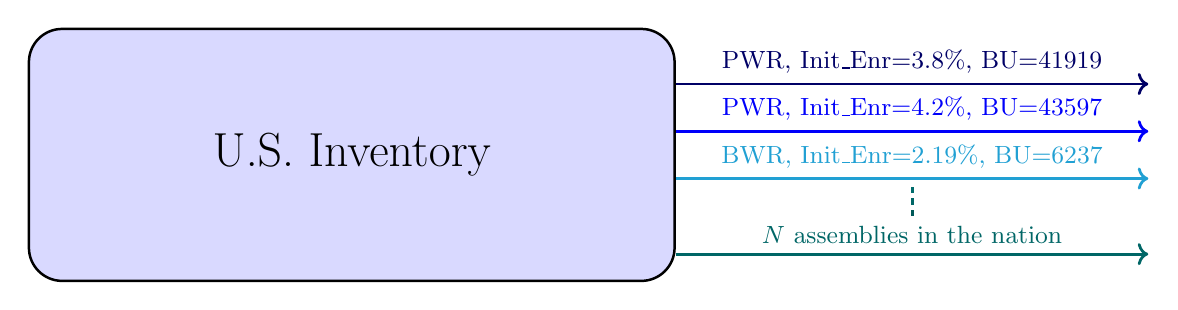
\begin{tikzpicture}[
    font=\rmfamily,
    box/.style={
        draw,
        rounded corners=12pt,
        line width=0.9pt,
        minimum width=8.2cm,
        minimum height=3.2cm,
        fill=blue!15,
        align=center
    },
    %, arrow styles (edit colors here), 
    a1/.style={->, line width=1pt, blue!40!black},
    a2/.style={->, line width=1pt, blue!98!black},
    a3/.style={->, line width=1pt, cyan!85!black},
    afinal/.style={->, line width=1pt, teal!80!black},
    %, consistent label style, 
    lab/.style={font=\small, align=center}
]

% Main box
\node[box] (inv) {\LARGE U.S. Inventory};

%, geometry controls, 
\def\arrowlen{6}        % arrow length to the right
\def\dy{0.6}            % equal spacing between arrows
\def\yone{0.9}          % top arrow offset (controls stack position)

% First three equally spaced arrows
\draw[a1] (inv.east) ++(0,\yone) -- ++(\arrowlen,0)
    node[midway, above, lab] {PWR, Init\_Enr=3.8\%, BU=41919};

\draw[a2] (inv.east) ++(0,\yone-\dy) -- ++(\arrowlen,0)
    node[midway, above, lab] {PWR, Init\_Enr=4.2\%, BU=43597};

\draw[a3] (inv.east) ++(0,\yone-2*\dy) -- ++(\arrowlen,0)
    node[midway, above, lab] {BWR, Init\_Enr=2.19\%, BU=6237};

% Three short vertical bars marking additional assemblies.
% They are drawn directly in the main picture to avoid nesting a tikzpicture.
\coordinate (continuation) at
    ($(inv.east)+(0.5*\arrowlen,\yone-2.5*\dy)$);
\draw[line width=1.1pt, teal!85!black]
    ($(continuation)+(0,0.19)$) -- ($(continuation)+(0,0.11)$);
\draw[line width=1.1pt, teal!80!black]
    ($(continuation)+(0,0.05)$) -- ($(continuation)+(0,-0.03)$);
\draw[line width=1.1pt, teal!70!black]
    ($(continuation)+(0,-0.10)$) -- ($(continuation)+(0,-0.18)$);

% Last arrow (different color) + label
\draw[afinal] (inv.east) ++(0,\yone-3.6*\dy) -- ++(\arrowlen,0)
    node[midway, above, lab] {$N$ assemblies in the nation};

\end{tikzpicture}
}
\caption{Structure of the U.S. Inventory module based on the STANDARDS~5.0.1 dataset. Representative PWR and BWR assemblies are identified by their initial enrichment, burnup, and isotopic composition, and the module retains all assemblies in the national spent fuel inventory.}
\label{fig:usinv-structure}
\end{figure}

\subsection{Purpose and Assembly-Level Data Source}
\label{subsec:us-inventory-data}

The source data are assembly-level records derived from \gls{STANDARDS}~5.0.1,
which associates individual U.S. spent fuel assemblies with facility, storage,
irradiation history, and calculated isotopic information. This level of detail
distinguishes assemblies that would otherwise be represented using an average
composition for a facility or for the national inventory
\cite{peterson_additional_2017,abdelkawy_summary_2025}.

For the simulations in this thesis, the \gls{STANDARDS} data were provided as a
directory of 75 line-delimited files, one per represented facility. The file
count is not hard-coded: the \texttt{data\_dir} parameter names a directory, and
every file whose name ends in \texttt{.txt} or contains \texttt{.jsonl} is read,
so the archetype can run on a subset of the database without recompilation.

Each nonempty line is one assembly record, converted into assembly metadata and a
nuclide mass map. Because the export wraps each dictionary-like record in an outer
JSON string, a purpose-built parser removes that wrapper and accepts both single-
and double-quoted strings. It reads the facility name, storage location name,
assembly identifier, storage type, discharge year, initial enrichment, maximum
burnup, initial uranium mass, and a dictionary of nuclide masses in grams.
Unrecognized fields are ignored, and records with no nonzero composition are
skipped.

The nuclide names are converted to the integer \texttt{ZZAAAM} identifiers used by
\Cyclus and assembled into a \texttt{cyclus::Composition}; the total assembly mass
is converted from grams to kilograms and stored with the record. Each assembly is
held in an \texttt{assembly} structure, summarized in Table~\ref{tab:usinv-bin}.

\begin{table}[h!]
    \centering
    \caption{Fields stored in each \texttt{assembly} structure.}
    \label{tab:usinv-bin}
    \begin{tabular}{p{0.34\textwidth} p{0.58\textwidth}}
        \hline
        \textbf{Field} & \textbf{Description} \\
        \hline
        Assembly\_ID          & Original database assembly identifier. \\
        Facility, location    & Source facility and storage location names. \\
        Storage type          & Wet or dry storage. \\
        Available mass        & Current material mass, in kilograms. \\
        Discharge year        & Year the assembly was discharged. \\
        Maximum burnup        & Reported maximum burnup. \\
        Initial enrichment    & Initial uranium enrichment. \\
        Initial uranium mass  & Initial mass of uranium. \\
        Derived fractions     & Fissile, plutonium, and minor actinide
        mass fractions. \\
        Coordinates           & Latitude and longitude of the source facility. \\
        Composition           & Complete \Cyclus composition of the assembly. \\
        \hline
    \end{tabular}
\end{table}

Because the original identifier is not unique across the dataset, the archetype
builds an internal key from the facility name, storage location, original
identifier, and load position, stored in \texttt{assembly\_id}; the raw value is
kept in \texttt{orig\_id}. Each assembly's available mass starts as the sum of its
reported nuclide masses, and a running total tracks the material remaining in the
facility.

Three composition fractions used by the selection policies are computed once at
load time. For assembly \(a\) with total mass \(m_a\) and nuclide mass
\(m_{i,a}\) for nuclide \(i\), the fissile mass fraction is

\begin{equation}
    f_{\mathrm{fissile},a}
    =
    \frac{
        m_{^{233}\mathrm{U},a}
        + m_{^{235}\mathrm{U},a}
        + m_{^{239}\mathrm{Pu},a}
        + m_{^{241}\mathrm{Pu},a}
    }{m_a},
    \label{eq:usinv-fissile-fraction}
\end{equation}

where the numerator sums the masses of \({}^{233}\mathrm{U}\),
\({}^{235}\mathrm{U}\), \({}^{239}\mathrm{Pu}\), and \({}^{241}\mathrm{Pu}\) in
assembly \(a\), and \(m_a\) is its total mass. The total plutonium mass fraction
is

\begin{equation}
    f_{\mathrm{Pu},a}
    =
    \frac{\displaystyle\sum_{i \in \mathrm{Pu}}m_{i,a}}{m_a},
    \label{eq:usinv-pu-fraction}
\end{equation}

where the sum runs over all plutonium isotopes present in assembly \(a\). The
minor actinide mass fraction is

\begin{equation}
    f_{\mathrm{MA},a}
    =
    \frac{
        \displaystyle
        \sum_{i \in \mathrm{Np}}m_{i,a}
        + \sum_{i \in \mathrm{Am}}m_{i,a}
        + \sum_{i \in \mathrm{Cm}}m_{i,a}
    }{m_a},
    \label{eq:usinv-ma-fraction}
\end{equation}

where each sum runs over all isotopes of neptunium, americium, or curium in
assembly \(a\). These fractions are precomputed so the selection policies need not
traverse the full nuclide composition on every request.

The required inputs are the output commodity, \texttt{outcommod}, and the
assembly data directory, \texttt{data\_dir}. An optional maximum throughput,
\texttt{throughput\_kg}, in kilograms per time step, is effectively unlimited by
default but can be reduced to represent a constraint on inventory retrieval,
transportation, or processing.

\subsection{Assembly Provenance and Geographic Coordinates}
\label{subsec:us-inventory-provenance}

Preserving assembly provenance connects inventory selection results to later
transportation, siting, and infrastructure analyses. The \gls{STANDARDS} records
identify each assembly's facility and storage location but not its coordinates,
so an optional SQLite database associates a facility name with latitude and
longitude.

The database path is supplied through \texttt{coordinates\_file}. If it is empty,
the archetype still runs but every assembly keeps the default pair \((0,0)\). When a
database is provided, it is opened read-only and queried for the facility name,
taking an exact match where one exists and otherwise a prefix match. All
assemblies from a facility share one coordinate pair, cached after the first
lookup. If no entry matches, the archetype warns and leaves that facility at
\((0,0)\).

Every completed transfer is recorded in a custom \Cyclus output table,
\texttt{us\_inventorySupply}, with one row per supplied trade
(Table~\ref{tab:usinv-supply}). The transferred material separately carries the
composition built from the selected assembly, so a transaction can be traced to both
its source assembly and its material composition.

\begin{table}[h!]
    \centering
    \caption{Columns written to the \texttt{us\_inventorySupply} output table.}
    \label{tab:usinv-supply}
    \begin{tabular}{p{0.34\textwidth} p{0.58\textwidth}}
        \hline
        \textbf{Column} & \textbf{Description} \\
        \hline
        Agent ID          & Identifier of the supplying agent. \\
        Time              & Simulation time step of the transfer. \\
        Facility          & Source facility name. \\
        Storage location  & Source storage location name. \\
        Storage type      & Wet or dry storage. \\
        Assembly ID       & Original assembly identifier. \\
        Initial uranium   & Initial uranium mass of the assembly. \\
        Latitude, longitude & Coordinates of the source facility. \\
        Quantity          & Mass supplied in the trade. \\
        Selection policy  & Policy in force for the simulation. \\
        \hline
    \end{tabular}
\end{table}

\subsection{Assembly Selection Policies}
\label{subsec:us-inventory-policies}

The archetype's principal methodological feature is its ability to choose among
individual assemblies by explicit ranking policies. In resource exchange the
solver decides which offers and requests match, but the supplier still chooses
which physical resource fulfills an accepted trade; \texttt{us\_inventory} uses
this selection step to model different assumptions about access to the legacy
inventory.

The policy is set through \texttt{selection\_policy} and checked at
initialization, where an unrecognized value stops the simulation with a
descriptive input error. For each trade the archetype scans the eligible assemblies and
keeps the one ranked highest under the active criterion, skipping empty assemblies and
assemblies without a valid composition. Table~\ref{tab:usinv-selection-policies} lists
the 15 policies.

\begin{table}[h!]
    \centering
    \caption{Assembly selection policies implemented by the
    \texttt{us\_inventory} archetype. Each policy ranks the eligible
    assemblies before a trade is fulfilled.}
    \label{tab:usinv-selection-policies}
    \begin{tabular}{p{0.34\textwidth} p{0.58\textwidth}}
        \hline
        \textbf{Policy} & \textbf{Assembly selected} \\
        \hline
        \texttt{first}                    & First eligible assembly in the database. \\
        \texttt{older}                    & Earliest discharge year. \\
        \texttt{newer}                    & Latest discharge year. \\
        \texttt{highest\_burnup}          & Largest reported maximum burnup. \\
        \texttt{lowest\_burnup}           & Smallest reported maximum burnup. \\
        \texttt{highest\_enrichment}      & Largest initial enrichment. \\
        \texttt{lowest\_enrichment}       & Smallest initial enrichment. \\
        \texttt{highest\_initial\_uranium}& Largest initial uranium mass. \\
        \texttt{lowest\_initial\_uranium} & Smallest initial uranium mass. \\
        \texttt{highest\_fissile}         & Largest fissile fraction
        (Eq.~\ref{eq:usinv-fissile-fraction}). \\
        \texttt{lowest\_fissile}          & Smallest fissile fraction. \\
        \texttt{highest\_plutonium}       & Largest plutonium fraction
        (Eq.~\ref{eq:usinv-pu-fraction}). \\
        \texttt{lowest\_plutonium}        & Smallest plutonium fraction. \\
        \texttt{highest\_minor\_actinide} & Largest minor actinide fraction
        (Eq.~\ref{eq:usinv-ma-fraction}). \\
        \texttt{lowest\_minor\_actinide}  & Smallest minor actinide fraction. \\
        \hline
    \end{tabular}
\end{table}

Ranking keeps the first eligible assembly as the initial candidate and replaces it
only when a later assembly is strictly better under the criterion, so ties retain their
load order priority.

Two optional inputs bias the pool toward a particular source.
\texttt{preferred\_facility} names a specific facility, and \texttt{storage\_type}
restricts the pool to \texttt{wet} or \texttt{dry} storage. These filters are
preferential rather than exclusive: the matching assemblies are searched first,
and if they cannot supply a trade the rest of the inventory is searched, with a
warning the first time this fallback occurs. This keeps the archetype consistent
with the \gls{DRE}, which expects a bidding facility to remain able to supply an
accepted trade.

Whether a request may be partially filled is governed by \texttt{allow\_partial}.
Selection first requires that an assembly cover the full requested mass; only if none
can, and \texttt{allow\_partial} is true, is a smaller quantity permitted.
Each accepted trade is drawn from a single assembly. The archetype does not combine
undersized assemblies, which preserves a one-to-one relationship between each trade
response and the assembly recorded in \texttt{us\_inventorySupply}.

\subsection{Material Bidding, Trading, and Accounting}
\label{subsec:us-inventory-accounting}

Bidding and trading are handled in two stages: the facility first advertises how
much material it can offer, and then, once trades are awarded, withdraws a
specific assembly for each one.

When there are requests on the output commodity, the facility bids. Because the
source filters are preferential, the whole remaining inventory is eligible, so the
facility can fall back to nonmatching assemblies. The compositions of the eligible
assemblies are combined into a single mass-weighted bid composition,

\begin{equation}
    \mathbf{x}_{\mathrm{bid}}
    =
    \frac{
        \displaystyle\sum_{a \in \mathcal{E}} m_a\,\vec{\mathbf{m}_a}
    }{
        \displaystyle\sum_{a \in \mathcal{E}} m_a
    },
    \label{eq:usinv-bid-composition}
\end{equation}

where \(\mathcal{E}\) is the set of eligible assemblies, \(m_a\) is the remaining mass of
assembly \(a\), and \(\vec(\mathbf{m}_a)\) is its vector of nuclide mass fractions. The
maximum mass offered is

\begin{equation}
    M_{\mathrm{offer}}
    =
    \min\!\left(
        M_{\mathrm{eligible}},\;
        M_{\mathrm{throughput}}
    \right),
    \label{eq:usinv-offer-capacity}
\end{equation}

where \(M_{\mathrm{eligible}} = \sum_{a \in \mathcal{E}} m_a\) is the total mass of
the eligible pool and \(M_{\mathrm{throughput}}\) is the configured
throughput per time step. This value enters the portfolio as a capacity
constraint. With partial fulfillment disabled, the archetype does not bid on a
request larger than it can offer.

The bid composition represents the available pool but does not replace
selection of the source assembly according to the active policy. After the
solver awards trades,
each one is matched to a source assembly by the procedure in
Section~\ref{subsec:us-inventory-policies}, so the material returned is built from
the selected assembly's composition, not the averaged bid composition.

Each accepted trade is limited by the requested quantity, the selected assembly's
remaining mass, and the throughput remaining in the step, and fulfillment stops
once the throughput or the inventory is exhausted. After each response the
archetype updates

\begin{align}
    m_{a,t+1}
    &= m_{a,t} - m_{\mathrm{supplied}},
    \label{eq:usinv-bin-update} \\
    M_{\mathrm{inv},t+1}
    &= M_{\mathrm{inv},t} - m_{\mathrm{supplied}},
    \label{eq:usinv-inv-update} \\
    R_{t+1}
    &= R_{t} - m_{\mathrm{supplied}},
    \label{eq:usinv-throughput-update}
\end{align}

where \(m_{a,t}\) is the available mass of the selected assembly \(a\),
\(M_{\mathrm{inv},t}\) is the total mass remaining in the facility, \(R_t\) is the
throughput remaining in the current step, and \(m_{\mathrm{supplied}}\) is the mass
delivered by the trade.

The remaining mass of each assembly is also persisted as archetype state, with
one value stored for every loaded assembly. Restarting from a checkpoint
reloads the assembly metadata
and compositions from the source files, overwrites their initial masses with the
persisted values, and rebuilds the inventory total from them. The simulation is
stopped if the number of persisted values does not match the number of loaded
assemblies, since that indicates the data directory changed after the checkpoint.

After each successful transaction the archetype appends a row to
\texttt{us\_inventorySupply}, giving a time-dependent history of which assemblies
were selected, where they originated, how much they supplied, and which policy
produced that sequence. These records form the basis for the policy
comparisons in Chapter~\ref{ch:results}.

%%%%%%%%%%%%%%%%%%%%%%%%%%%%%%%%%%%%%%%%%%%%%%%%%%%%%%%%%%%%%%%%%%%%%%%%%%%%%%%%%%%%%%%%%%%%%%%%%%%%%%%%%%%%%%%%%%%%%%%%%%%%%%%%%
%%%%%%%%%%%%%%%%%%%%%%%%%%%%%%%%%%%%%%%%%%%%%%%%%%%%%%%%%%%%%%%%%%%%%%%%%%%%%%%%%%%%%%%%%%%%%%%%%%%%%%%%%%%%%%%%%%%%%%%%%%%%%%%%%
%%%%%%%%%%%%%%%%%%%%%%%%%%%%%%%%%%%%%%%%%%%%%%%%%%%%%%%%%%%%%%%%%%%%%%%%%%%%%%%%%%%%%%%%%%%%%%%%%%%%%%%%%%%%%%%%%%%%%%%%%%%%%%%%%
\section{The \texttt{ads} Archetype}
\label{sec:ads-archetype}

The archetype represents an \gls{ADS} operating as a transuranic
burner. It receives an actinide-bearing feed from upstream facilities,
accumulates one core loading, irradiates it for a prescribed cycle, and
discharges the surviving actinides together with the fission products generated
during the cycle. Like \texttt{us\_inventory}
(Section~\ref{sec:us-inventory-archetype}), it inherits from
\texttt{cyclus::Facility}. Unlike \texttt{us\_inventory}, it does not use the
\texttt{CommodityProducer} toolkit class; instead, it explicitly requests feed,
bids its discharged product, advances an irradiation cycle each time step, and
participates in the \gls{DRE} on both the request and bid sides.
Its input feed and output commodity streams are illustrated in
Figure~\ref{fig:ads-structure}.

\begin{figure}[h!]
\centering
\resizebox{0.95\textwidth}{!}{%
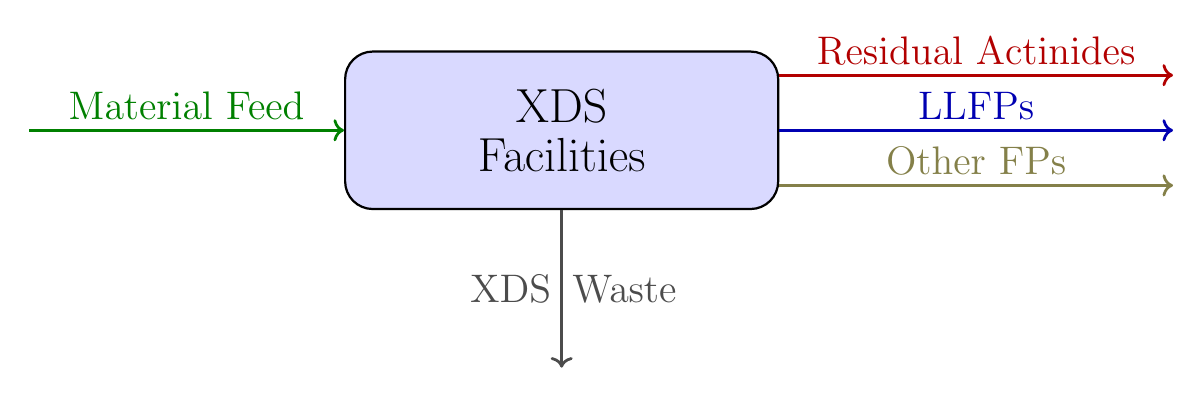
\begin{tikzpicture}[
font=\rmfamily,
box/.style={
    draw,
    rounded corners=10pt,
    line width=0.8pt,
    fill=blue!15,
    minimum width=5.5cm,
    minimum height=2cm,
    align=center
},
inputarrow/.style={->, line width=1pt, green!50!black},
actarrow/.style={->, line width=1pt, red!70!black},
llfparrow/.style={->, line width=1pt, blue!70!black},
fparrow/.style={->, line width=1pt, yellow!45!black},
wastearrow/.style={->, line width=1pt, black!70}
]

% Main box
\node[box] (xds) {\LARGE XDS\\[2mm]\LARGE Facilities};

% Input arrow
\draw[inputarrow] ($(xds.west)+(-4,0)$) -- (xds.west)
    node[midway, above] {\Large Material Feed};

% ===== Output arrows =====

% Top-right output
\draw[actarrow] (xds.east) ++(0,0.7) -- ++(5,0)
    node[midway, above] {\Large Residual Actinides};

% Middle-right output
\draw[llfparrow] (xds.east) -- ++(5,0)
    node[midway, above] {\Large LLFPs};

% Bottom-right output
\draw[fparrow] (xds.east) ++(0,-0.7) -- ++(5,0)
    node[midway, above] {\Large Other FPs};

% Bottom output
\draw[wastearrow] (xds.south) -- ++(0,-2)
    node[midway, left] {\Large XDS}
    node[midway, right] {\Large Waste};

\end{tikzpicture}
}
\caption{Structure of the \gls{XDS} facility archetype within the \Cyclus
framework, showing the input material feed and the output streams containing
residual actinides, long-lived fission products, other fission products, and
waste.}
\label{fig:ads-structure}
\end{figure}

\subsection{Reduced-Order Transmutation Model}
\label{subsec:ads-reduced-order}

Solving neutron transport and depletion throughout a fuel cycle simulation
that spans several decades, for every cycle of every burner, is computationally
intractable. The
\texttt{ads} archetype therefore uses a \emph{reduced-order} model: the physics is
computed once, offline, by high-fidelity depletion calculations, and at runtime
the archetype performs only a case lookup and an interpolation. This mirrors the
recipe-based treatment of irradiation established in \Cyclus
\cite{huff_fundamental_2016}.

The offline physics is a library of \textsc{Serpent} depletion cases
(Section~\ref{subsec:serpent-cases}), each recording the time evolution of the
full nuclide inventory of a fixed loading irradiated at constant power. The
library is loaded once when the agent enters the simulation and held in memory.

\paragraph{Buffers and cycle.}
The facility holds three material buffers: \texttt{feed} accumulates received
material, \texttt{core} holds the loading under irradiation, and \texttt{product}
holds discharged material awaiting trade. The feed and core buffers share the
\texttt{capacity} parameter, the mass of one core, while the product buffer is
unbounded. Operation is a two-state batch cycle keyed on whether the core is
occupied. An empty core is refueling; once \texttt{refuel\_time} has elapsed and
the feed holds a full core, one \texttt{capacity} of feed is loaded. An occupied
core irradiates until its cycle counter reaches \texttt{cycle\_time}, at which
point it is discharged. The composition is not altered during irradiation.
Instead, the entire transformation is applied as a single transition at
discharge because the core does not participate in resource exchange while
loaded. Two persisted
counters track progress through the irradiation and refueling periods so the
operating state survives a simulation snapshot.

\paragraph{Feed requests.}
Feed may be requested on several input commodities listed in \texttt{incommods},
with an optional preference assigned to each commodity. The archetype requests
the available space in its feed buffer, and the requests for the different
commodities are mutually exclusive alternatives in one portfolio. It therefore
draws one core load from whichever supplier the exchange prefers rather than the
full amount from each. An optional \texttt{feed\_recipe} may be attached; when it is empty, the request is
for blank material and the archetype accepts whatever composition the supplier
offers. This is the mode used here, since the feed composition varies with the
inventory selection policy and with any upstream separations.

\paragraph{Simulation time to irradiation time.}
\Cyclus advances in time steps, whereas the \textsc{Serpent} cases are tabulated in
irradiation days. The parameter \texttt{days\_per\_step}, $\Delta_d$, converts
between them, so the irradiation time read at discharge is

\begin{equation}
    t_{\mathrm{irr}} = n_{\mathrm{cycle}}\,\Delta_d,
    \label{eq:ads-tirr}
\end{equation}

where $n_{\mathrm{cycle}}$ is the cycle length in time steps
(\texttt{cycle\_time}). If $\Delta_d$ is not set, it is derived from the time step
duration. This is what gives the cycle length physical meaning: a longer cycle
addresses a later, more-depleted point on the trajectory.

\paragraph{Case selection.}
At discharge the core is matched to the library case that best represents it. The
core is reduced to the mass fractions of three actinide groups, normalized to the
total actinide mass:

\begin{equation}
    f_{\mathrm{MA}} = \frac{m_{\mathrm{Np}}+m_{\mathrm{Am}}+m_{\mathrm{Cm}}}
                           {m_{\mathrm{act}}},
    \quad
    f_{\mathrm{Pu}} = \frac{m_{\mathrm{Pu}}}{m_{\mathrm{act}}},
    \quad
    f_{\mathrm{U}}  = \frac{m_{\mathrm{U}}}{m_{\mathrm{act}}},
    \label{eq:ads-fractions}
\end{equation}

where each element mass ($m_{\mathrm{Np}}$, $m_{\mathrm{Am}}$, $m_{\mathrm{Cm}}$,
$m_{\mathrm{Pu}}$, $m_{\mathrm{U}}$) is summed over all isotopes of that element,
$m_{\mathrm{act}} = \sum_{Z\geq 89} m$ is the total actinide mass, and the minor
actinides are neptunium, americium, and curium. Nuclides below $Z = 89$ are
excluded, so fission products in recycled feed do not affect selection. The same
fractions are computed for each case from its initial ($t=0$) actinide vector.
Each case $c$ is scored by

\begin{equation}
    S_c = w_P\,\frac{\lvert P - P_c\rvert}{\max(P,\,P_c)}
          + \sum_{g \in \{\mathrm{MA},\,\mathrm{Pu},\,\mathrm{U}\}}
            \lvert f_g - f_{g,c}\rvert,
    \label{eq:ads-score}
\end{equation}

where $P$ and $P_c$ are the facility and case powers, $f_g$ and $f_{g,c}$ are the
core and case group fractions, and $w_P = 10$ weights the power term. The
case with the lowest score is selected; the large $w_P$ makes the power tier
dominate, so a core is not matched across power levels on composition alone. A
single nearest case is chosen. There is no averaging across cases, and
interpolation occurs only along that case's time axis.

\paragraph{Composition transformation.}
\label{subsec:ads-discharge}
The selected case gives nuclide masses $m_n(t_k)$ at tabulated times $t_k$. For
the interval $[t_{\mathrm{lo}}, t_{\mathrm{hi}}]$ bracketing $t_{\mathrm{irr}}$,
each nuclide is linearly interpolated,

\begin{equation}
    m_n(t_{\mathrm{irr}}) = (1-\alpha)\,m_n(t_{\mathrm{lo}})
                          + \alpha\,m_n(t_{\mathrm{hi}}),
    \qquad
    \alpha = \frac{t_{\mathrm{irr}} - t_{\mathrm{lo}}}
                  {t_{\mathrm{hi}} - t_{\mathrm{lo}}},
    \label{eq:ads-interp}
\end{equation}

over every actinide and fission product the case tracks, and the result becomes
the discharged composition. Outside the tabulated range the composition is clamped
to the nearest endpoint rather than extrapolated: depletion saturates as the most
fissile nuclides are consumed, so a straight-line projection past the last point
would overpredict burnup and eventually yield negative masses. A cycle that
routinely runs past the range signals a misconfigured time mapping or a need for
longer depletion runs, not a case for extrapolation.

\paragraph{Mass balance.}
The transformed composition holds both surviving actinides and the fission
products made during irradiation, so mass is conserved to the extent
\textsc{Serpent} tracks it. With $M(t)$ the total tracked (actinide plus
fission product) mass of the case at time $t$, the discharged mass scales from the
loading $M_{\mathrm{in}}$ by

\begin{equation}
    R = \min\!\left(1,\ \frac{M(t_{\mathrm{irr}})}{M(0)}\right),
    \qquad
    M_{\mathrm{out}} = R\,M_{\mathrm{in}},
    \label{eq:ads-ratio}
\end{equation}

the upper limit of unity prevents a ratio slightly greater than one from
creating mass. The residual $(1-R)\,M_{\mathrm{in}}$ leaves the simulation as a
recorded mass defect, representing mass not retained in the \textsc{Serpent} output
tables, including mass converted to energy during fission and any light or
otherwise untracked nuclides. Writing
$a_c(t) = M_{\mathrm{act},c}(t)/M_c(t)$ for the actinide fraction
of the matched case, the destroyed actinide mass reported for the cycle is

\begin{equation}
    \Delta M_{\mathrm{act}} =
        M_{\mathrm{in}}\,a_c(0) - M_{\mathrm{out}}\,a_c(t_{\mathrm{irr}}).
    \label{eq:ads-destroyed}
\end{equation}

Equation~\ref{eq:ads-destroyed} measures the net reduction in total
actinide mass represented by the matched depletion case. Both
\(a_c(0)\) and \(a_c(t_{\mathrm{irr}})\) include the complete actinide inventory
reported in the Serpent actinide mass table. Consequently, conversion from one
actinide to another, for example, conversion of a minor actinide into
plutonium, does not count as destruction, because the product nuclide remains
in the discharged actinide inventory. This is a summary quantity only; the
discharged isotopics come directly from Equation~\ref{eq:ads-interp}. Discharged
material is then offered on the output commodity under a capacity constraint
equal to the product mass, and accepted trades draw from the product buffer for
routing to storage, separations, or disposal.

\subsection{Serpent Depletion Cases}
\label{subsec:serpent-cases}

These depletion cases were produced at \gls{UIUC} as part of the \gls{EINSTEIN}
project by Runxia Wen, of the neutronics analysis group led by Professor Tomasz
Kozlowski. This section documents the model they represent so that the
archetype's inputs can be interpreted. Each case is a continuous-energy
Serpent~2 Monte Carlo depletion calculation
\cite{leppanenStatusSerpentMonte2025} that tracks the full nuclide inventory
(\texttt{set inventory all}), producing the time-dependent actinide and
fission product mass tables the archetype later reads; the material volumes
required for depletion normalization are obtained by a Monte Carlo volume
calculation.

Figure~\ref{fig:serpent-geometry} shows the model geometry, an axisymmetric
cylindrical \gls{ADS} core built from concentric \(z\)-cylinders. Its principal
regions and dimensions are summarized in Table~\ref{tab:serpent-geometry}. A
central spallation target filled with liquid lead sits on the core midplane,
surrounded by a
thin structural target wall and, above it, an evacuated beam duct through which
the proton beam reaches the target. The fuel occupies the annular region around
the target tube, and the whole assembly is enclosed in structural material and
an outer container. A vacuum (black) boundary condition is applied at the
outermost surface, so neutrons leaking past the container are lost. The single
target, single homogeneous fuel region, and absence of detail at the assembly
or pin level are consistent with the reduced-order role of these cases: they are
intended to characterize the bulk transmutation behavior of one core load of
feed rather than its detailed spatial power distribution.

\begin{table}[h!]
    \centering
    \caption{Principal regions of the Serpent \gls{ADS} model. Dimensions are
    taken directly from the input decks; all cylinders are coaxial about the
    \(z\)-axis.}
    \label{tab:serpent-geometry}
    \footnotesize
    \begin{tabular}{p{0.24\textwidth} p{0.20\textwidth} p{0.20\textwidth} p{0.24\textwidth}}
        \hline
        \textbf{Region} & \textbf{Radius (cm)} & \textbf{Axial span (cm)} &
        \textbf{Material} \\
        \hline
        Spallation target & 0--17.5   & 150--210  & Liquid lead \\
        Beam duct (vacuum) & 0--17.5  & 210--400  & Void \\
        Target wall        & 17.5--18.5 & 149--400 & Structural \\
        Fuel               & 18.5--150 & 0--300    & Minor actinide feed\\
        Container / structure & 150--250 & \(-100\)--400 & Structural \\
        \hline
    \end{tabular}
\end{table}

\begin{figure}[h!]
\centering
% To resize, change the x/y unit lengths below (keep them equal to stay to-scale).
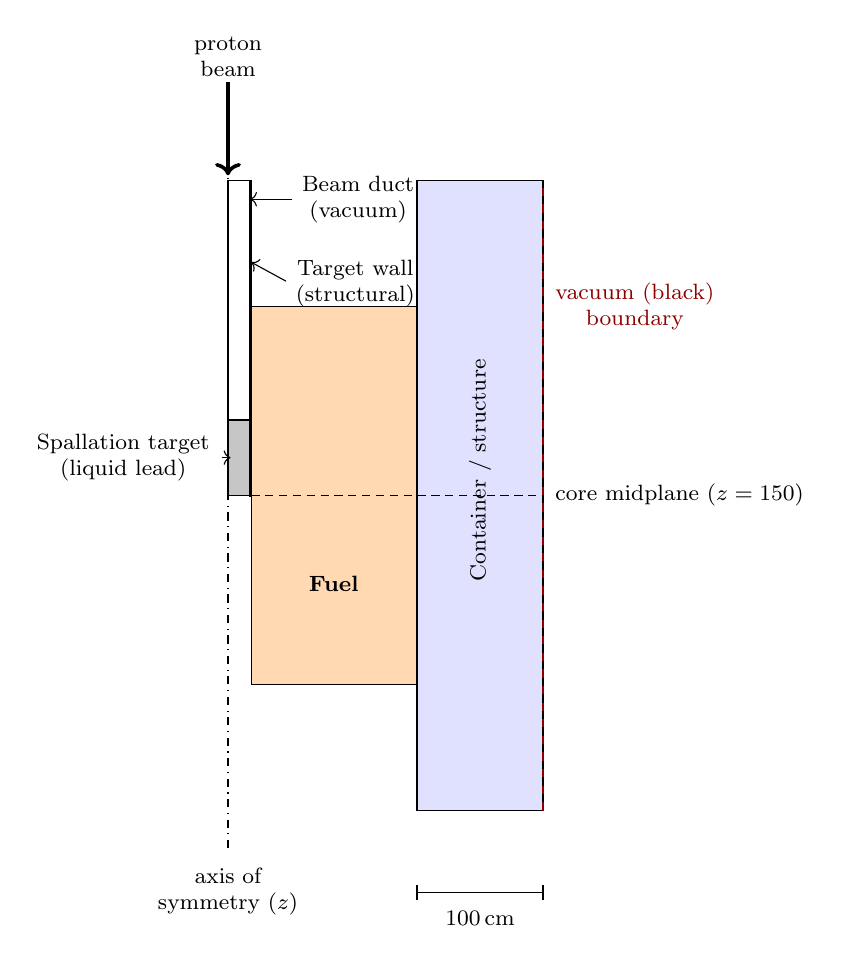
\begin{tikzpicture}[
    x=0.016cm, y=0.016cm,
    font=\footnotesize,
    region/.style={draw=black, line width=0.5pt},
    lead/.style={->, line width=0.4pt},
    lab/.style={align=center}
]

% ---- regions (half r--z section, r >= 0), values from Table~\ref{tab:serpent-geometry} ----
\draw[region, fill=blue!12]   (150,-100) rectangle (250,400); % Container / structure
\draw[region, fill=orange!30] (18.5,0)   rectangle (150,300); % Fuel
\draw[region, fill=gray!70]   (17.5,149) rectangle (18.5,400);% Target wall
\draw[region, fill=white]     (0,210)    rectangle (17.5,400);% Beam duct (void)
\draw[region, fill=gray!45]   (0,150)    rectangle (17.5,210);% Spallation target

% ---- axis of symmetry (= z-axis) ----
\draw[dash dot, line width=0.4pt] (0,-130) -- (0,430);
\node[below, lab] at (0,-138) {axis of\\symmetry ($z$)};

% ---- proton beam ----
\draw[->, line width=1.3pt] (0,478) -- (0,404);
\node[lab] at (0,498) {proton\\beam};

% ---- core midplane ----
\draw[densely dashed, line width=0.4pt] (18.5,150) -- (250,150);
\node[right] at (252,150) {core midplane ($z=150$)};

% ---- vacuum (black) boundary ----
\draw[dashed, line width=0.9pt, red!55!black] (250,-100) -- (250,400);
\node[right, lab, text=red!55!black] at (252,300) {vacuum (black)\\boundary};

% ---- region labels ----
\node[lab] at (84,80) {\textbf{Fuel}};
\node[lab, rotate=90] at (200,170) {Container / structure};

\draw[lead] (-5,180) -- (2,180);
\node[left, lab] at (-7,180) {Spallation target\\(liquid lead)};

\draw[lead] (51,385) -- (17.5,385);
\node[right, lab] at (51,385) {Beam duct\\(vacuum)};

\draw[lead] (46,320) -- (18.5,335);
\node[right, lab] at (46,318) {Target wall\\(structural)};

% ---- radial scale bar ----
\draw[line width=0.5pt] (150,-165) -- (250,-165);
\draw[line width=0.5pt] (150,-171) -- (150,-159);
\draw[line width=0.5pt] (250,-171) -- (250,-159);
\node[below] at (200,-172) {$100\,\mathrm{cm}$};

\end{tikzpicture}
\caption[Serpent \gls{ADS} core geometry.]{To-scale half cross-section
($r$--$z$) of the axisymmetric Serpent \gls{ADS} model, mirrored about the
axis of symmetry. Concentric regions and dimensions are taken from
Table~\ref{tab:serpent-geometry}: a central spallation target filled with
liquid lead on the core midplane, an evacuated beam duct above it, a thin structural target
wall, the surrounding fuel annulus, and the outer container. A vacuum (black)
boundary condition is applied at the outermost surface.}
\label{fig:serpent-geometry}
\end{figure}

\subsubsection{Fuel Compositions and the Case Set}
\label{subsubsec:serpent-materials}

The cases differ in the composition loaded into the fuel region, which is what
makes them a \emph{library} rather than a single run. Each fuel is a transuranic
feed dispersed in a lead matrix. Two representative cases illustrate the range
spanned by the library. In one, the feed is essentially pure minor actinide
dispersed in lead; in another, the feed contains equal masses of plutonium
and minor actinides in lead. These two feeds bracket the
transmutation regimes of interest: a charge containing only minor actinides
maximizes the
minor actinide mass destroyed in each cycle but presents the greatest
reactivity challenge during loading, whereas adding plutonium reduces that
challenge while shifting some of the
destruction burden onto bred and fissioned plutonium. The initial actinide mass
of each case, taken from the day-zero row of its actinide mass table, is the
quantity the archetype's \texttt{capacity} parameter should reproduce, so that a
loaded core matches the case it is compared against.

Each case is depleted along a common ``\(\mathrm{Day}~[\mathrm{d}]\)'' time axis.
The irradiation history is built up from a sequence of chained restart runs: an
initial segment resolves the first fraction of a day with fine steps (for
example, cumulative times of \(0.001\), \(0.1\), \(0.2\), and
\(0.5~\mathrm{d}\)) to capture the rapid early transient in short-lived
fission products, and each subsequent segment reads the binary restart file
written by the previous one and advances the total burnup further (for example,
from \(730\) to \(760~\mathrm{d}\)). Reassembled, these segments give the
continuous nuclide inventory versus irradiation time that the archetype consumes:
an actinide mass table (\texttt{plot\_data\_15\_actinide\_masses\_full.txt} or
\texttt{plot\_data\_06\_actinide\_masses.txt}), a fission product mass table
(\texttt{plot\_data\_14\_fission\_product\_masses.txt}) on the same axis, and a
power history (\texttt{plot\_data\_03\_power\_vs\_time.txt}) used for case
matching. The archetype reads a case's composition at the irradiation time
implied by the cycle length by linearly interpolating these tables along the
day axis, so the resolution of the discharged composition is set by the density
of the Serpent time grid rather than by the \Cyclus time step.

\subsection{Irradiation Event Recording}
\label{subsec:ads-events}

Besides the standard \Cyclus tables, the archetype writes a custom
\texttt{AdsEvents} table so each cycle can be reconstructed without parsing the
full isotopic history. Every row carries the agent ID, time, event type, matched
case, and a mass value (Table~\ref{tab:ads-events}); the matched case is blank on
a load, since matching happens at discharge.

\begin{table}[h!]
    \centering
    \caption{Event types recorded in the \texttt{AdsEvents} output table.}
    \label{tab:ads-events}
    \begin{tabular}{p{0.26\textwidth} p{0.66\textwidth}}
        \toprule
        \textbf{Event} & \textbf{Recorded value} \\
        \midrule
        \texttt{Load} & Mass loaded from feed into the core. \\
        \texttt{Discharge} & Core mass entering the transformation,
                             $M_{\mathrm{in}}$, before Equation~\ref{eq:ads-ratio};
                             the matched case is recorded here. \\
        \texttt{ActinideDestroyed} & Destroyed actinide mass,
                             Equation~\ref{eq:ads-destroyed}. \\
        \texttt{FissionProducts} & Fission product mass in the discharged material. \\
        \texttt{MassDefect} & Mass not retained, $(1-R)\,M_{\mathrm{in}}$. \\
        \bottomrule
    \end{tabular}
\end{table}

The three discharge rows are written only when positive. The
\texttt{ActinideDestroyed} series is the primary performance metric, and its
cumulative sum gives the actinide mass a facility removes from the fuel cycle. With
the standard \Cyclus \texttt{Transactions} and \texttt{ExplicitInventory} tables,
these events close the actinide balance: the actinide initially present equals the
sum destroyed, held in buffers, and resident downstream.

%%%%%%%%%%%%%%%%%%%%%%%%%%%%%%%%%%%%%%%%%%%%%%%%%%%%%%%%%%%%%%%%%%%%%%%%%%%%%%%%%%%%%%%%%%%%%%%%%%%%%%%%%%%%%%%%%%%%%%%%%%%%%%%%%
%%%%%%%%%%%%%%%%%%%%%%%%%%%%%%%%%%%%%%%%%%%%%%%%%%%%%%%%%%%%%%%%%%%%%%%%%%%%%%%%%%%%%%%%%%%%%%%%%%%%%%%%%%%%%%%%%%%%%%%%%%%%%%%%%
%%%%%%%%%%%%%%%%%%%%%%%%%%%%%%%%%%%%%%%%%%%%%%%%%%%%%%%%%%%%%%%%%%%%%%%%%%%%%%%%%%%%%%%%%%%%%%%%%%%%%%%%%%%%%%%%%%%%%%%%%%%%%%%%%

\section{Simulation Scenarios}
\label{sec:simulation-scenarios}

The two archetypes developed in this chapter are exercised in a set of
fuel cycle simulations that share one flowsheet and differ along three axes: the
composition burned in the \gls{ADS}, the length of the simulated horizon, and
whether the discharged material is recycled. Two burner configurations are used,
corresponding to the two representative Serpent cases described in
Section~\ref{subsec:serpent-cases}: a core containing only minor actinides
(ADS~1) and a core containing equal masses of plutonium and minor actinides
(ADS~2). Each configuration is simulated over 30-year and 100-year horizons in
both once-through and recycling modes, resulting in eight simulations.

\subsection{Fuel Cycle Flow}
\label{subsec:scenario-flowsheet}

Every simulation uses the same chain of facilities. The \texttt{us\_inventory}
facility supplies discharged assemblies on the \texttt{snf} commodity under the
\texttt{highest\_minor\_actinide} selection policy
(Section~\ref{subsec:us-inventory-policies}), so that the assemblies richest in
neptunium, americium, and curium are drawn first. A \Cycamore
\texttt{Separations} facility partitions this material: the minor actinides are
routed to the burner feed, while uranium, plutonium (except in ADS~2), and the
fission products fall to a leftover stream sent to a waste \texttt{Sink}. The
\gls{ADS} irradiates the separated feed and discharges the surviving actinides
together with the fission products produced during the cycle. Depending on the
scenario, that discharge is either sent to a \texttt{Sink} (once-through) or
returned to \texttt{Separations} (recycling).

The two burner configurations shape the feed differently. For
ADS~1, which contains only minor actinides, \texttt{Separations} extracts a
single stream of neptunium, americium, and curium at \(99\%\) efficiency and feeds it directly
to the \gls{ADS}. For ADS~2, which contains equal masses of plutonium and minor actinides, the
feed cannot be taken straight from separations: the U.S. inventory holds roughly ten times more
plutonium than minor actinide, so a stream drawn from it is far from an equal
split. \texttt{Separations} therefore produces two streams, one of minor
actinides and one of plutonium, and a \Cycamore \texttt{Mixer} blends them in a
fixed \(0.5/0.5\) mass ratio to reproduce the ADS~2 Serpent feed. The minor
actinide stream limits the feed rate, so surplus plutonium
accumulates in its buffer. This limitation arises from the composition of the
inventory rather than from an imposed modeling constraint.

The separations facilities in these scenarios are idealized material
partitioning models. The simulations assume that an operating reprocessing
system can recover plutonium and the minor actinides into distinct product
streams at the specified \(99\%\) efficiencies. This is an enabling boundary
condition of the analysis rather than a prediction of deployable process
performance. The \textsc{Cycamore} \texttt{Separations} archetype applies
user defined partitioning efficiencies but does not represent process
chemistry, product purity, decontamination factors, plant availability,
secondary waste generation, remote fabrication of actinide bearing fuel,
safeguards, licensing, or the broader policy constraints associated with
commercial reprocessing. The results therefore describe the material flow
performance of the ADS scenarios conditional on such separations
infrastructure being available.

The recycling and once-through modes differ only in the routing of the burner
discharge. In once-through mode the discharge is a terminal waste stream held in
a \texttt{Sink}. In recycling mode it is returned to \texttt{Separations}, which
recovers the surviving minor actinides, and, for ADS~2, plutonium, into fresh
feed, so that actinides make repeated passes through the burner while uranium and
fission products are removed to waste on each pass.

The two routings are shown in Figure~\ref{fig:flowsheet-oncethrough} for the
once-through cycle and Figure~\ref{fig:flowsheet-recycle} for the recycling cycle.

\begin{sidewaysfigure}[h!]
\centering
\resizebox{0.96\linewidth}{!}{%
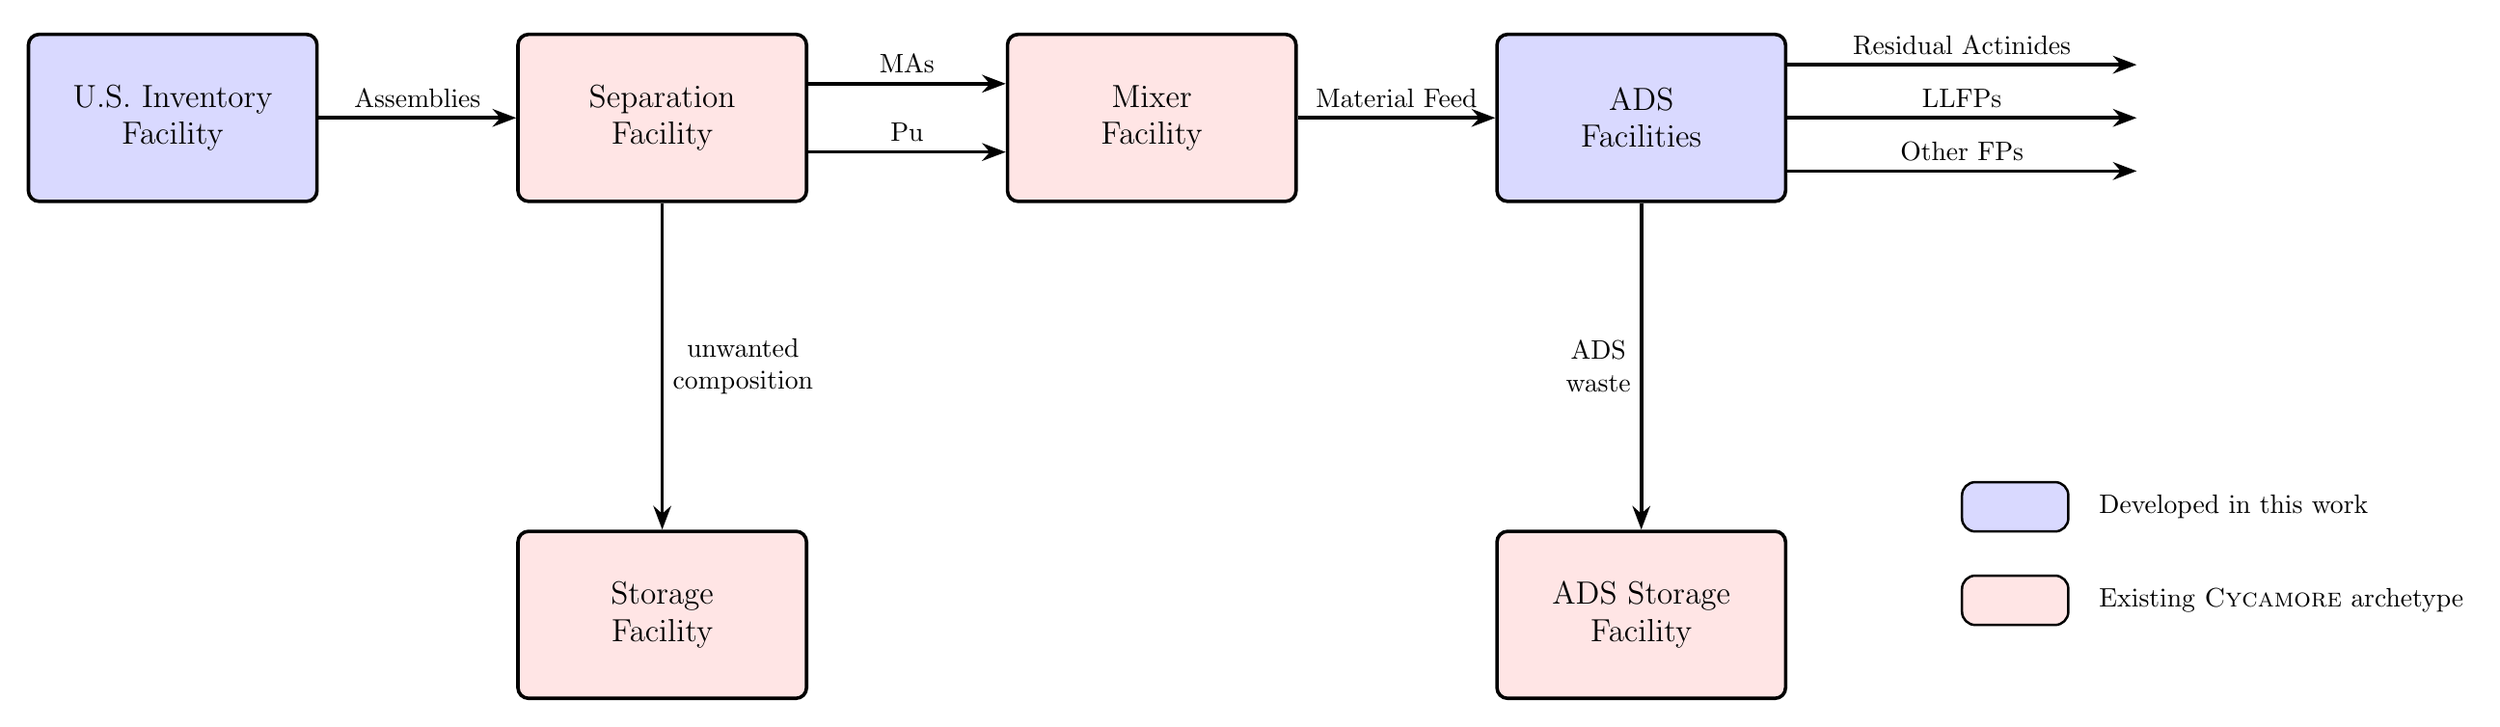
\begin{tikzpicture}[
    >=Stealth,
    font=\large,
    node distance=2.6cm,
    every path/.style={line width=1.3pt},
    block/.style={
        draw,
        rounded corners,
        minimum width=3.8cm,
        minimum height=2.2cm,
        line width=1.3pt,
        align=center
    },
    blueblock/.style={block, fill=blue!15},
    pinkblock/.style={block, fill=red!10},
    annot/.style={font=\normalsize, align=center},
    keybox/.style={draw, rounded corners=5pt, minimum width=1.4cm,
                   minimum height=0.65cm, line width=0.9pt}
]

\node[blueblock] (inv) {U.S. Inventory\\Facility};
\node[pinkblock, right=of inv] (sep) {Separation\\Facility};
\node[pinkblock, right=of sep] (mix) {Mixer\\Facility};
\node[blueblock, right=of mix] (ads) {ADS\\Facilities};

\node[pinkblock, below=4.3cm of sep] (stor_sep) {Storage\\Facility};
\node[pinkblock, below=4.3cm of ads] (stor_ads) {ADS Storage\\Facility};

\draw[->] (inv) -- node[midway, above, annot]{Assemblies} (sep);

\draw[->] ([yshift=0.45cm]sep.east) -- ([yshift=0.45cm]mix.west)
    node[midway, above, annot]{MAs};
\draw[->] ([yshift=-0.45cm]sep.east) -- ([yshift=-0.45cm]mix.west)
    node[midway, above, annot]{Pu};

\draw[->] (mix) -- node[midway, above, annot]{Material Feed} (ads);

\draw[->] (sep.south) -- (stor_sep.north)
    node[midway, right, annot]{unwanted\\composition};
\draw[->] (ads.south) -- (stor_ads.north)
    node[midway, left, annot]{ADS\\waste};

\draw[->] ([yshift=0.70cm]ads.east) -- ++(4.6cm,0)
    node[midway, above, annot]{Residual Actinides};
\draw[->] (ads.east) -- ++(4.6cm,0)
    node[midway, above, annot]{LLFPs};
\draw[->] ([yshift=-0.70cm]ads.east) -- ++(4.6cm,0)
    node[midway, above, annot]{Other FPs};

% Legend, drawn directly in the same TikZ picture.
\node[keybox, fill=blue!15] (keyblue)
    at ([xshift=3.0cm,yshift=-4.0cm]ads.south east) {};
\node[anchor=west, font=\normalsize]
    at ([xshift=0.25cm]keyblue.east) {Developed in this work};
\node[keybox, fill=red!10, below=0.55cm of keyblue] (keypink) {};
\node[anchor=west, font=\normalsize]
    at ([xshift=0.25cm]keypink.east) {Existing \textsc{Cycamore} archetype};

\end{tikzpicture}%
}
\caption[Once-through fuel cycle flowsheet.]{Conceptual flow for the
once-through fuel cycle. Material from the \gls{STANDARDS}~5.0.1 inventory is
separated, blended when needed, and irradiated in the \gls{ADS}. Separation
waste and \gls{ADS} discharge products follow separate terminal storage paths.
Blue facilities denote archetypes developed for this work, while pink
facilities represent existing \textsc{Cycamore} archetypes.}
\label{fig:flowsheet-oncethrough}
\end{sidewaysfigure}

\begin{sidewaysfigure}[h!]
\centering
\resizebox{0.96\linewidth}{!}{%
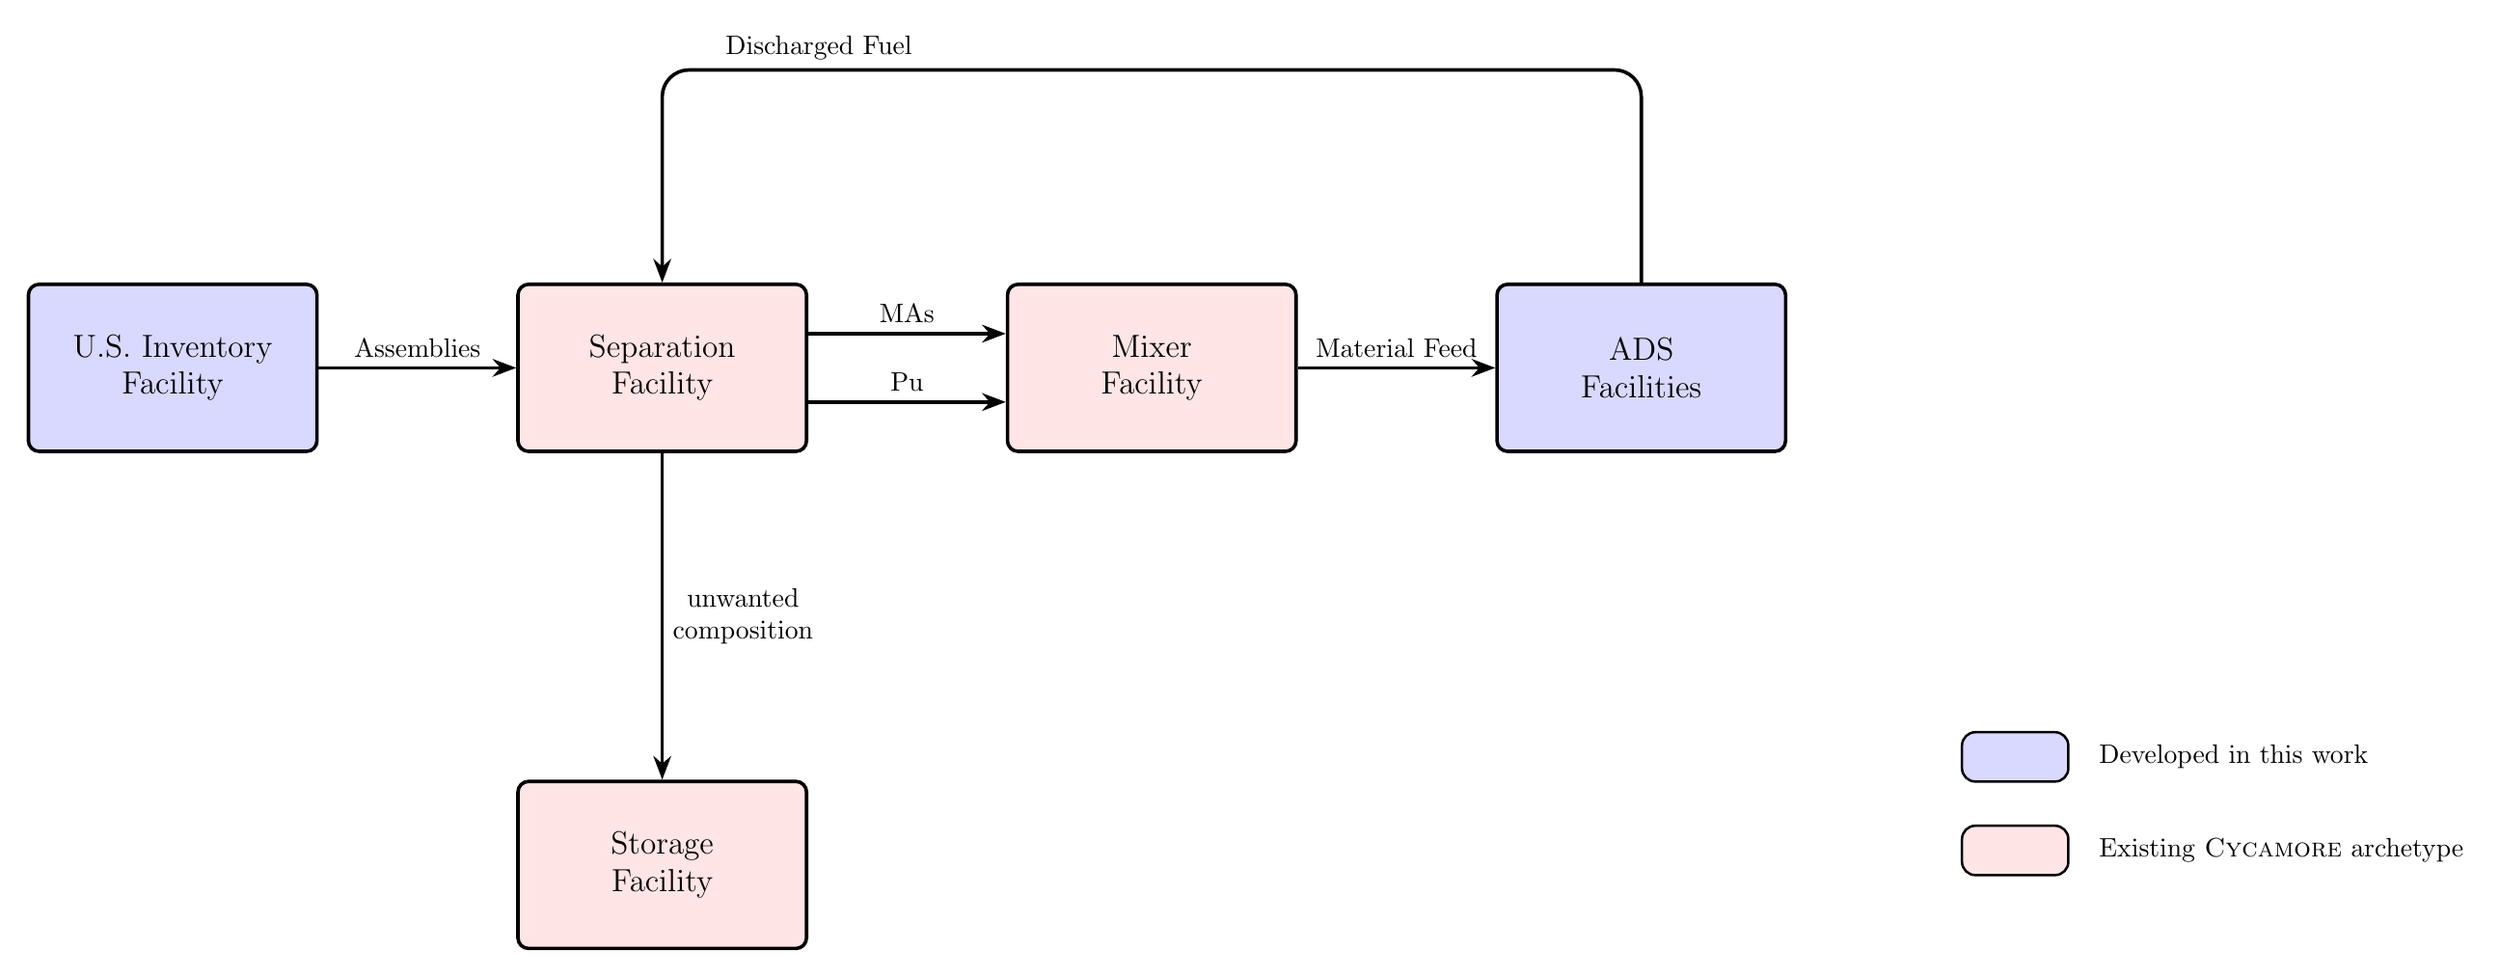
\begin{tikzpicture}[
    >=Stealth,
    font=\large,
    node distance=2.6cm,
    every path/.style={line width=1.3pt},
    block/.style={
        draw,
        rounded corners,
        minimum width=3.8cm,
        minimum height=2.2cm,
        line width=1.3pt,
        align=center
    },
    blueblock/.style={block, fill=blue!15},
    pinkblock/.style={block, fill=red!10},
    annot/.style={font=\normalsize, align=center},
    keybox/.style={draw, rounded corners=5pt, minimum width=1.4cm,
                   minimum height=0.65cm, line width=0.9pt}
]

\node[blueblock] (inv) {U.S. Inventory\\Facility};
\node[pinkblock, right=of inv] (sep) {Separation\\Facility};
\node[pinkblock, right=of sep] (mix) {Mixer\\Facility};
\node[blueblock, right=of mix] (ads) {ADS\\Facilities};

\node[pinkblock, below=4.3cm of sep] (stor_sep) {Storage\\Facility};

\draw[->] (inv) -- node[midway, above, annot]{Assemblies} (sep);

\draw[->] ([yshift=0.45cm]sep.east) -- ([yshift=0.45cm]mix.west)
    node[midway, above, annot]{MAs};
\draw[->] ([yshift=-0.45cm]sep.east) -- ([yshift=-0.45cm]mix.west)
    node[midway, above, annot]{Pu};

\draw[->] (mix) -- node[midway, above, annot]{Material Feed} (ads);

\draw[->] (sep.south) -- (stor_sep.north)
    node[midway, right, annot]{unwanted\\composition};

\draw[->, rounded corners=10pt]
    (ads.north) -- ++(0,2.8cm) -| (sep.north)
    node[pos=0.42, above, annot]{Discharged Fuel};

% Legend, drawn directly in the same TikZ picture.
\node[keybox, fill=blue!15] (keyblue)
    at ([xshift=3.0cm,yshift=-4.0cm]ads.south east) {};
\node[anchor=west, font=\normalsize]
    at ([xshift=0.25cm]keyblue.east) {Developed in this work};
\node[keybox, fill=red!10, below=0.55cm of keyblue] (keypink) {};
\node[anchor=west, font=\normalsize]
    at ([xshift=0.25cm]keypink.east) {Existing \textsc{Cycamore} archetype};

\end{tikzpicture}%
}
\caption[Recycling fuel cycle flowsheet.]{Conceptual flow for the closed
(recycling) fuel cycle. Material from the \gls{STANDARDS}~5.0.1 inventory is
separated, blended when needed, and irradiated in the \gls{ADS}; the discharged
fuel is then returned to the separation facility for recovery and reuse. The
unwanted separation stream is sent to storage. Blue facilities denote
archetypes developed for this work, while pink facilities represent existing
\textsc{Cycamore} archetypes.}
\label{fig:flowsheet-recycle}
\end{sidewaysfigure}

All simulations share the remaining settings. Time advances in monthly steps of
\(30.4375~\mathrm{d}\) from a start of January~2025, radioactive decay is
evaluated lazily over the horizon, and explicit inventory tracking is enabled.
The inventory, separations, and mixing facilities each operate at a throughput of
\(250{,}000~\mathrm{kg}\) per step, large enough that material handling does not
throttle the burner.

\subsection{Simulation Runs}
\label{subsec:scenario-runs}

The two burner configurations fix the \gls{ADS} and separations parameters
summarized in Table~\ref{tab:scenario-config}. Each core mass matches the
day-zero actinide mass of the corresponding Serpent case, so a loaded core maps
onto the case it is compared against; the cycle lengths differ by more than the
mass alone, as the large core containing only minor actinides is irradiated
for ten years per cycle while the smaller \(50/50\) core is cycled every two years.

\begin{table}[h!]
    \centering
    \caption{\gls{ADS} and separations configuration for the two burner cases.
    Cycle and refueling times are given in monthly time steps, with the
    equivalent duration in parentheses.}
    \label{tab:scenario-config}
    \begin{tabular}{p{0.30\textwidth} p{0.27\textwidth} p{0.27\textwidth}}
        \hline
        \textbf{Parameter} & \textbf{Case 3 (MA only)} &
        \textbf{Case 4 (50/50 Pu--MA)} \\
        \hline
        Initial core mass  & \(27{,}000~\mathrm{kg}\) & \(4{,}418~\mathrm{kg}\) \\
        Cycle length       & 120 steps (10 yr)       & 24 steps (2 yr) \\
        Refueling time     & 6 steps (6 mo)          & 4 steps (4 mo) \\
        Power level        & \(3000~\mathrm{MW}\)    & \(3000~\mathrm{MW}\) \\
        Separated streams  & Np, Am, Cm              & Np, Am, Cm and Pu \\
        Feed shaping       & Fed directly            &
        \Cycamore \texttt{Mixer}, \(0.5/0.5\) \\
        Serpent case       & \texttt{892\_vt\_ma\_Pb} &
        \texttt{1.3\_vt\_5050\_puma\_Pb} \\
        \hline
    \end{tabular}
\end{table}

Each configuration is simulated over both horizons and in both modes, giving the
eight runs listed in Table~\ref{tab:scenario-runs}. Across most of these runs the
once-through and recycling modes produce nearly identical histories, because the
burner is limited by its cycle duration rather than by feed availability.
Within the horizon, it completes the same number of cores whether or not the discharge is recycled, and the
recovered material only displaces inventory that was still available. The
exception is ADS~1 over the 100-year horizon. Its large core load and ten-year
irradiation cycle draw down the accessible minor actinide inventory, and
recycling allows operation to continue beyond what the once-through supply can
support. The comparison between recycling and once-through in Chapter~\ref{ch:results}
therefore focuses on that pair of runs; for the remaining cases a single
representative run is shown, since the two modes coincide.

\begin{table}[h!]
    \centering
    \caption{Simulation runs. Each burner configuration is run over both
    horizons and in both fuel management modes.}
    \label{tab:scenario-runs}
    \begin{tabular}{c l l l c}
        \hline
        \textbf{Run} & \textbf{Fuel case} & \textbf{Mode} &
        \textbf{Horizon} & \textbf{Steps} \\
        \hline
        1 & MA only      & Once-through & 30 yr  & 360  \\
        2 & MA only      & Recycle      & 30 yr  & 360  \\
        3 & MA only      & Once-through & 100 yr & 1200 \\
        4 & MA only      & Recycle      & 100 yr & 1200 \\
        5 & 50/50 Pu--MA & Once-through & 30 yr  & 360  \\
        6 & 50/50 Pu--MA & Recycle      & 30 yr  & 360  \\
        7 & 50/50 Pu--MA & Once-through & 100 yr & 1200 \\
        8 & 50/50 Pu--MA & Recycle      & 100 yr & 1200 \\
        \hline
    \end{tabular}
\end{table}

\chapter{Results}
\label{ch:results}
\section{Inventory Characterization}
\label{sec:results-baseline}

Before any transmutation results are presented, this section characterizes the
inventory that the \texttt{us\_inventory} archetype ingests, establishing both
that the \gls{STANDARDS}~5.0.1 dataset is loaded correctly and the scale and
distribution of the material available to the fuel cycle. Because the inventory
load is deterministic, the same directory of assembly records always produces
the same pool, these results depend only on the input data and the parser, not
on any simulation dynamics.

Reading the 75 assembly-record files yields $315{,}976$ individual assemblies,
totalling $8.69\times10^{4}~\mathrm{t}$ of heavy metal, drawn from 61 facilities
for which geographic coordinates are available. Summing the minor-actinide
content of every assembly, as defined in Equation~\ref{eq:usinv-ma-fraction},
gives a total accessible minor-actinide inventory of $103.8~\mathrm{t}$. This
minor actinide is only $0.12\%$ of the total heavy metal, a consequence of the
low neptunium, americium, and curium content of discharged
light-water-reactor fuel. Put in terms of the burner, the entire national
minor-actinide inventory amounts to fewer than four \gls{ADS} cores at the
$27~\mathrm{t}$ core loading of the minor-actinide-only case
(Table~\ref{tab:scenario-config}). This scarcity is the central constraint on
the transmutation mission and recurs throughout the results: the burner is
limited far more by the availability of minor actinide than by any reactor
parameter.

Figure~\ref{fig:results-source-map} shows the geographic distribution of this
material, with each facility placed at its coordinates and shaded by the mass of
spent fuel it supplies over a full-horizon run. Because the run draws down the
accessible inventory, the drawn mass approaches the available inventory at each
site, so the figure doubles as a map of where the national inventory resides.
The distribution is strongly weighted toward the eastern and south-central
United States, where the largest single sites each supply on the order of
$2{,}500$--$2{,}700~\mathrm{t}$, while the smaller western sites contribute a few
hundred tonnes. This spatial concentration is the starting point for the
provenance analysis of Section~\ref{sec:results-policy}, since any policy that
draws assemblies in a particular order also implies a particular geographic
sequence of retrieval.

\begin{figure}[htbp]
  \centering
  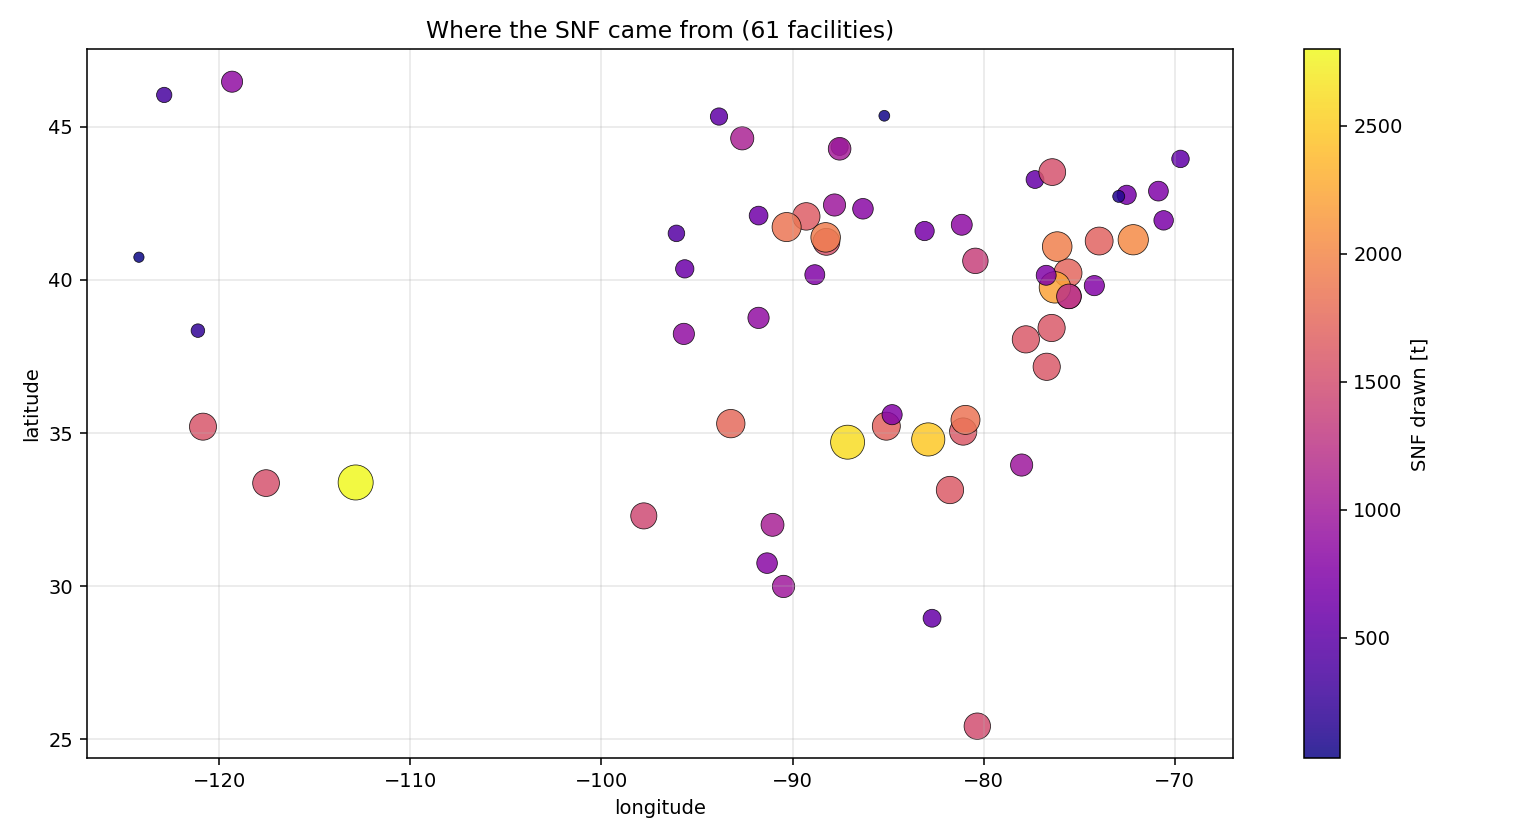
\includegraphics[width=0.95\textwidth]{figures/results_source_map}
  \caption[Geographic distribution of the sourced U.S.\ spent-fuel
  inventory.]{Geographic distribution of the spent nuclear fuel supplied by the
  \texttt{us\_inventory} archetype. Each marker is one of the 61 facilities with
  known coordinates, positioned by latitude and longitude and shaded and sized
  by the mass of spent fuel drawn over the full simulation horizon. The
  inventory is concentrated in the eastern and south-central United States.}
  \label{fig:results-source-map}
\end{figure}

Establishing this baseline confirms that the archetype ingests the assembly-level
dataset faithfully and quantifies the material the transmutation fuel cycle has
to work with. The remainder of this chapter examines how that material is
selected (Section~\ref{sec:results-policy}), how it is transmuted in the
\gls{ADS} (Section~\ref{sec:results-ads}), and how the accessible inventory
evolves under recycling (Section~\ref{sec:results-evolution}).

%%%%%%%%%%%%%%%%%%%%%%%%%%%%%%%%%%%%%%%%%%%%%%%%%%%%%%%%%%%%%%%%%%%%%%%%%%%%%%%%%%%%%%%%%%%%%%%%%%%%%%%%%%%%%%%%%%%%%%%%%%%%%%%%%
%%%%%%%%%%%%%%%%%%%%%%%%%%%%%%%%%%%%%%%%%%%%%%%%%%%%%%%%%%%%%%%%%%%%%%%%%%%%%%%%%%%%%%%%%%%%%%%%%%%%%%%%%%%%%%%%%%%%%%%%%%%%%%%%%
%%%%%%%%%%%%%%%%%%%%%%%%%%%%%%%%%%%%%%%%%%%%%%%%%%%%%%%%%%%%%%%%%%%%%%%%%%%%%%%%%%%%%%%%%%%%%%%%%%%%%%%%%%%%%%%%%%%%%%%%%%%%%%%%%

\section{Effect of Selection Policy on the Feed}
\label{sec:results-policy}

The \texttt{us\_inventory} archetype selects individual assemblies by an explicit
ranking policy (Section~\ref{subsec:us-inventory-policies}), and that choice
determines the mass and composition of material delivered to separations and,
ultimately, to the burner. The selection mechanism acts on the static inventory
pool and is deterministic in the assembly ordering it produces: it does not
depend on downstream reactor dynamics. Its effect on the feed can therefore be
characterized directly, from the inventory data and from standalone
\texttt{us\_inventory} runs, independently of the full fuel cycle, and that is
how it is presented in this section. The production scenarios of
Chapter~\ref{ch:results} all use \texttt{highest\_minor\_actinide}
(Section~\ref{subsec:scenario-flowsheet}); the comparisons here show what that
choice buys relative to the alternatives.

\subsection{Delivery Trajectory}
\label{subsec:results-policy-trajectory}

Because every policy eventually draws from the same finite pool, the total
minor actinide any policy can deliver is identical: the cumulative curves all
terminate at the same $103.8~\mathrm{t}$
(Section~\ref{sec:results-baseline}). What the policy changes is the
\emph{trajectory}, how quickly minor actinide accumulates as assemblies are
drawn. Figure~\ref{fig:results-policy-trajectory} shows the cumulative minor
actinide delivered against the number of assemblies drawn, for the three
representative policies of set~A, with a horizontal line marking one
$27~\mathrm{t}$ minor-actinide-only core.

The separation is large. Ranking by \texttt{highest\_minor\_actinide} reaches a
full core after roughly $4.8\times10^{4}$ assembly draws, whereas
\texttt{lowest\_minor\_actinide} requires about $1.28\times10^{5}$, a factor of
$2.7$ more material handled for the same core. The unranked \texttt{first}
baseline falls between them, at about $7.7\times10^{4}$ draws, and its curve is
visibly segmented: because \texttt{first} draws facility by facility in load
order, its slope steps up and down as it moves through sites of differing minor-
actinide quality, whereas the ranked policies produce smooth, monotonically
curving trajectories. The timing here is expressed in assemblies drawn rather
than calendar time, since the mapping to time depends on the per-step retrieval
throughput, which is not the subject of this comparison.

This is the practical face of the scarcity established in
Section~\ref{sec:results-baseline}. With the national inventory holding fewer
than four cores of minor actinide in total, the order of retrieval governs how
much spent fuel must be handled, and, as shown next, from how many sites, to
assemble even a single core.

\begin{figure}[htbp]
  \centering
  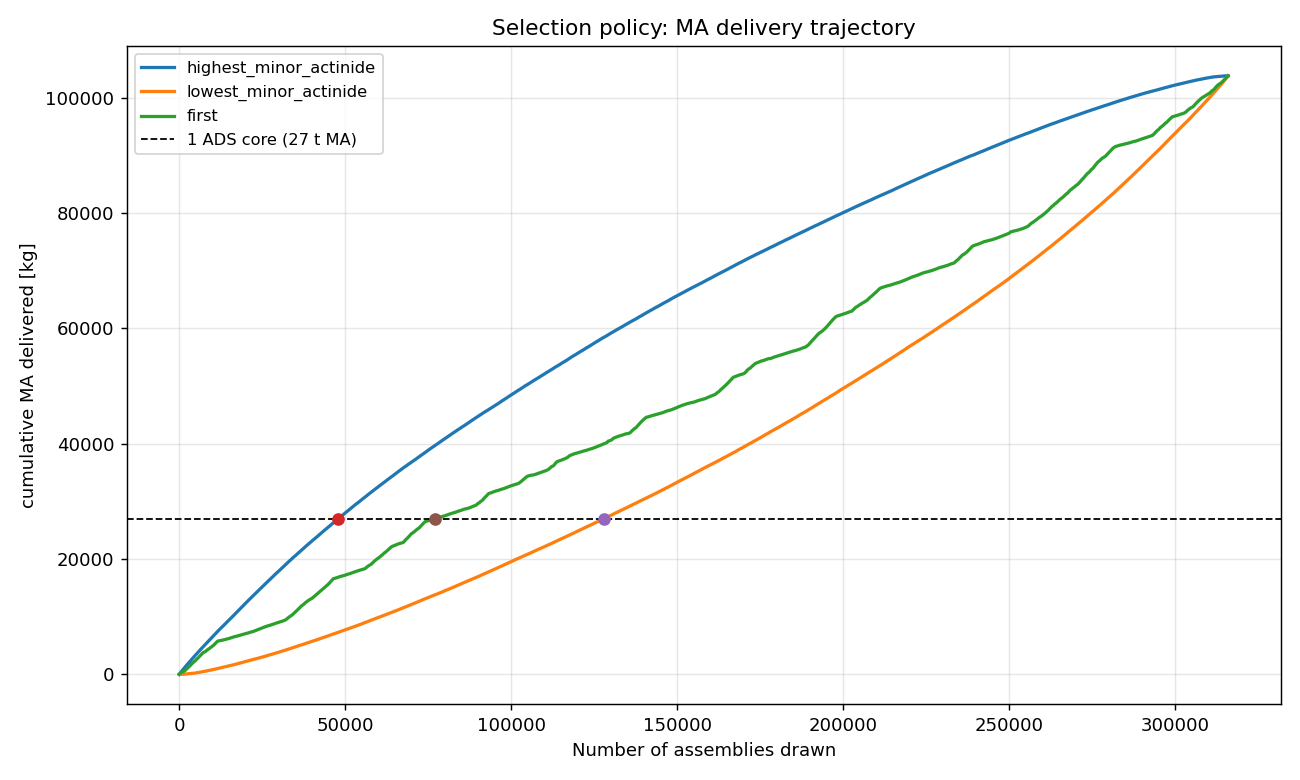
\includegraphics[width=0.9\textwidth]{figures/policy_trajectory}
  \caption[Minor-actinide delivery trajectory by selection policy.]{Cumulative
  minor actinide delivered as a function of assemblies drawn, for three
  selection policies. All policies terminate at the same total, since they draw
  from one finite pool; they differ only in how quickly minor actinide
  accumulates. The dashed line marks one $27~\mathrm{t}$ minor-actinide-only
  core; markers indicate where each policy first supplies a full core.
  \texttt{highest\_minor\_actinide} reaches a core with roughly $2.7$ times
  fewer draws than \texttt{lowest\_minor\_actinide}.}
  \label{fig:results-policy-trajectory}
\end{figure}

\subsection{Geographic Provenance of the Feed}
\label{subsec:results-policy-provenance}

Because the selection order is also a geographic order, each policy implies a
different set of sites supplying the first core.
Figure~\ref{fig:results-policy-provenance} shows the minor actinide contributed
by each facility to the first $27~\mathrm{t}$ core under the set~A policies.
The contrast is stark. The \texttt{first} policy, drawing in load order,
concentrates the core in a handful of sites, each contributing on the order of
$2~\mathrm{t}$; \texttt{highest\_minor\_actinide} instead spreads the draw across
many facilities, tapping the minor-actinide-rich assemblies wherever they
reside, so that no single site dominates. Ranking for feed quality thus trades a
geographically concentrated retrieval for a distributed one, a consideration
that connects directly to transportation and logistics, which fall outside the
scope of this work but are enabled by the provenance recorded in
\texttt{us\_inventorySupply} (Table~\ref{tab:usinv-supply}).

\begin{figure}[htbp]
  \centering
  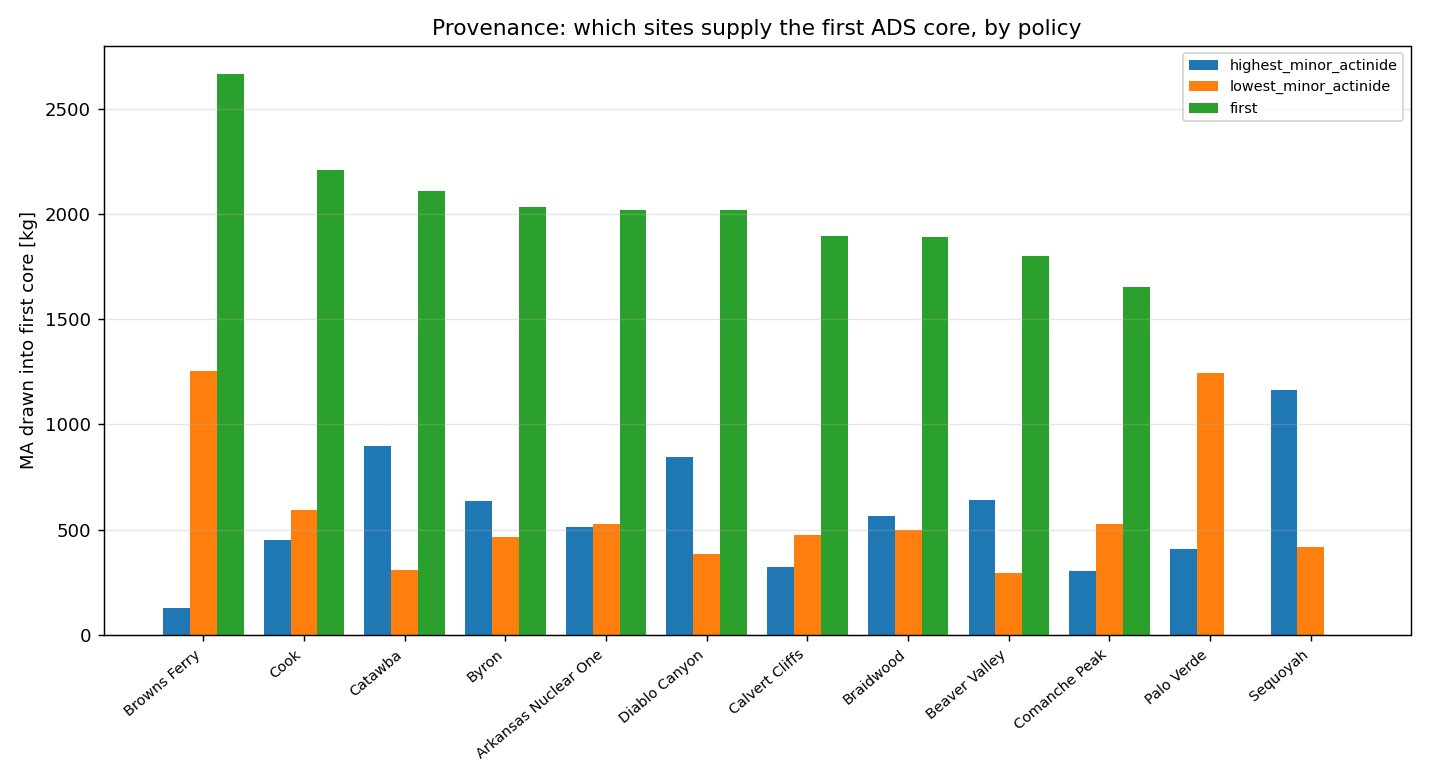
\includegraphics[width=0.95\textwidth]{figures/policy_provenance}
  \caption[Facility provenance of the first core by selection policy.]{Minor
  actinide contributed by each facility to the first $27~\mathrm{t}$ core, for
  the set~A policies. \texttt{first} concentrates the core in a few sites drawn
  in load order, while \texttt{highest\_minor\_actinide} distributes it across
  many facilities.}
  \label{fig:results-policy-provenance}
\end{figure}

The effect is not specific to minor-actinide ranking. When the pool is instead
ordered by discharge age (\texttt{older}, \texttt{newer}) or by reported burnup
(\texttt{highest\_burnup}, \texttt{lowest\_burnup}), the set of sites supplying
the first core shifts again, each policy favoring the facilities whose
assemblies rank highest under its criterion. This confirms that the archetype's
selection acts as a general lever on feed provenance: any physical property
recorded in the assembly data can be used to reshape both the composition and
the geographic origin of the material entering the fuel cycle.

Finally, that the mechanism operates identically inside a full \Cyclus
simulation, not only in offline analysis of the pool, was confirmed in a
standalone \texttt{us\_inventory} run in which the average composition of the
supplied material tracked the active policy, with plutonium- and
burnup-ranked policies delivering the correspondingly higher plutonium and
fissile fractions expected from the ranking.


%%%%%%%%%%%%%%%%%%%%%%%%%%%%%%%%%%%%%%%%%%%%%%%%%%%%%%%%%%%%%%%%%%%%%%%%%%%%%%%%%%%%%%%%%%%%%%%%%%%%%%%%%%%%%%%%%%%%%%%%%%%%%%%%%
%%%%%%%%%%%%%%%%%%%%%%%%%%%%%%%%%%%%%%%%%%%%%%%%%%%%%%%%%%%%%%%%%%%%%%%%%%%%%%%%%%%%%%%%%%%%%%%%%%%%%%%%%%%%%%%%%%%%%%%%%%%%%%%%%
%%%%%%%%%%%%%%%%%%%%%%%%%%%%%%%%%%%%%%%%%%%%%%%%%%%%%%%%%%%%%%%%%%%%%%%%%%%%%%%%%%%%%%%%%%%%%%%%%%%%%%%%%%%%%%%%%%%%%%%%%%%%%%%%%

\section{ADS Transmutation Performance}
\label{sec:results-ads}

This section examines how the \gls{ADS} transmutes the separated feed. Of the
eight runs defined in Section~\ref{subsec:scenario-runs}, most coincide: as
anticipated there, the once-through and recycling modes produce nearly identical
histories wherever the burner is cycle-limited rather than feed-limited, so a
single representative run suffices for those cases. The results therefore reduce
to two comparisons that isolate the physics of interest. The first contrasts the
two burner configurations, the minor-actinide-only core (ADS~1) and the
\(50/50\) plutonium-minor-actinide core (ADS~2), over the 100-year horizon,
establishing how core size and feed composition govern the burner's behavior. The
second contrasts recycling against once-through operation for the
minor-actinide-only core, the one pairing where the two modes diverge. Throughout,
the per-cycle transmutation physics is identical between modes and horizons; what
changes is how many cycles the burner completes before it exhausts its feed.

\subsection{Per-Cycle Transmutation and Burn Fraction}
\label{subsec:results-ads-burn}

At each discharge the core composition is read from the matched \textsc{Serpent}
case (Section~\ref{subsec:ads-discharge}), giving the surviving actinides and the
fission products produced during the cycle. Figures~\ref{fig:results-case3-recycle-fpyield}
and~\ref{fig:results-case4-recycle-fpyield} show the cumulative fission-product
yield of the two cores, plotted against fission-product mass number. Both are the
familiar double-humped curve of low-to-moderate-energy actinide fission, with a
light peak near \(A \approx 100\) and a heavy peak near \(A \approx 138\)
separated by the symmetric-fission valley. For the minor-actinide-only core
(Figure~\ref{fig:results-case3-recycle-fpyield}) this signature appears even though
the feed contains no uranium or plutonium, confirming that the minor actinides
themselves are fissioning in the fast, subcritical core: the double hump is a
property of the fission fragments' shell structure, not of which actinide split.
In both cases the three burnup snapshots nearly overlie one another, since the
cumulative yield shape is set by the actinide mixture, which shifts only slowly
with irradiation.

The two cores differ in the details of the distribution, and the difference
reflects their feed. The \(50/50\) core
(Figure~\ref{fig:results-case4-recycle-fpyield}) contains a large plutonium
fraction, and \({}^{239}\mathrm{Pu}\) fissions from a heavier compound nucleus
than the minor-actinide vector; heavier fissioning systems place the light peak
slightly higher in mass and fill in the symmetric valley, reducing the
peak-to-valley ratio. The minor-actinide-only core, fissioning a lighter mix
dominated by americium and neptunium, is consistent with a marginally deeper
valley and a light peak shifted slightly lower. The shift is subtle because both
feeds fission in the same fast spectrum and span overlapping actinide masses, but
it is the expected signature of a plutonium-bearing versus a plutonium-free feed,
and it confirms that the reduced-order model carries the compositional distinction
through to the fission-product inventory.

\begin{figure}[htbp]
  \centering
  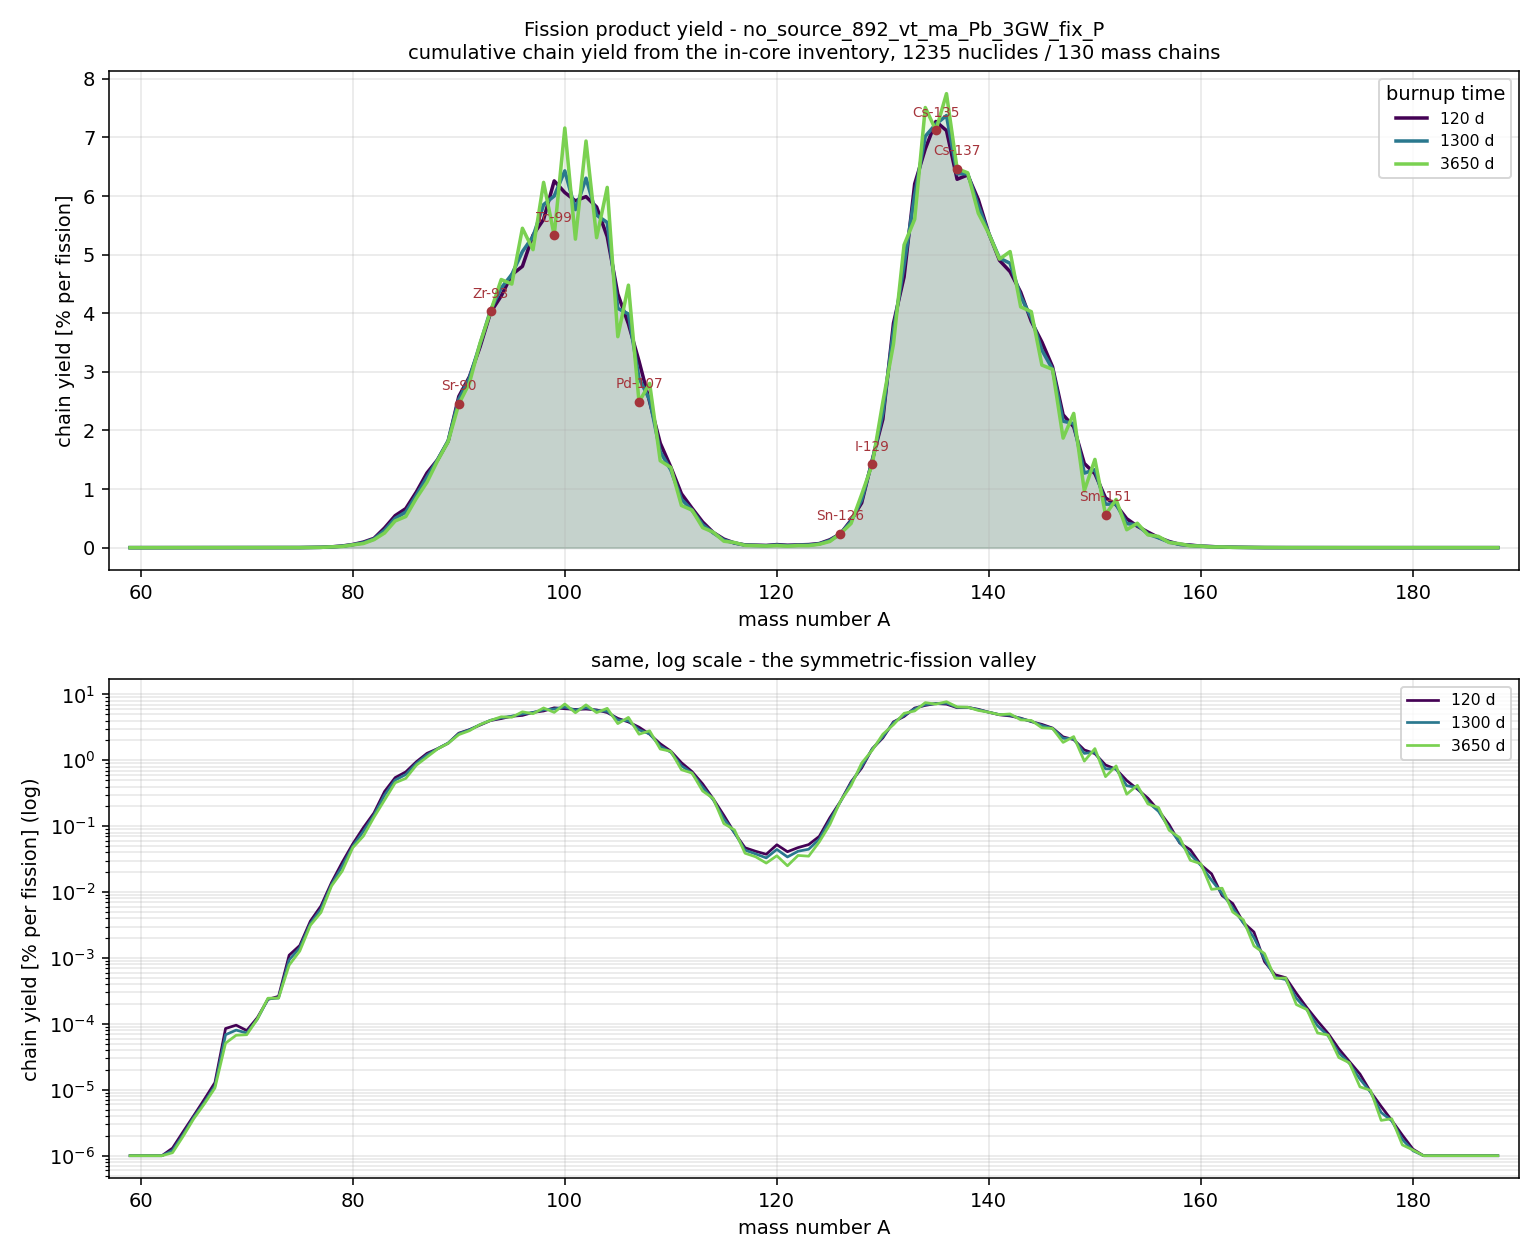
\includegraphics[width=0.9\textwidth]{figures/case3_ma_recycle_100yr_fp_yield}
  \caption[Fission-product yield of the minor-actinide-only core.]{Cumulative
  fission-product chain yield of the minor-actinide-only core (ADS~1) as a
  function of fission-product mass number, at three points in the irradiation. The
  double-humped distribution appears despite the absence of uranium or plutonium
  in the feed, confirming that the minor actinides are the fissioning species.}
  \label{fig:results-case3-recycle-fpyield}
\end{figure}

\begin{figure}[htbp]
  \centering
  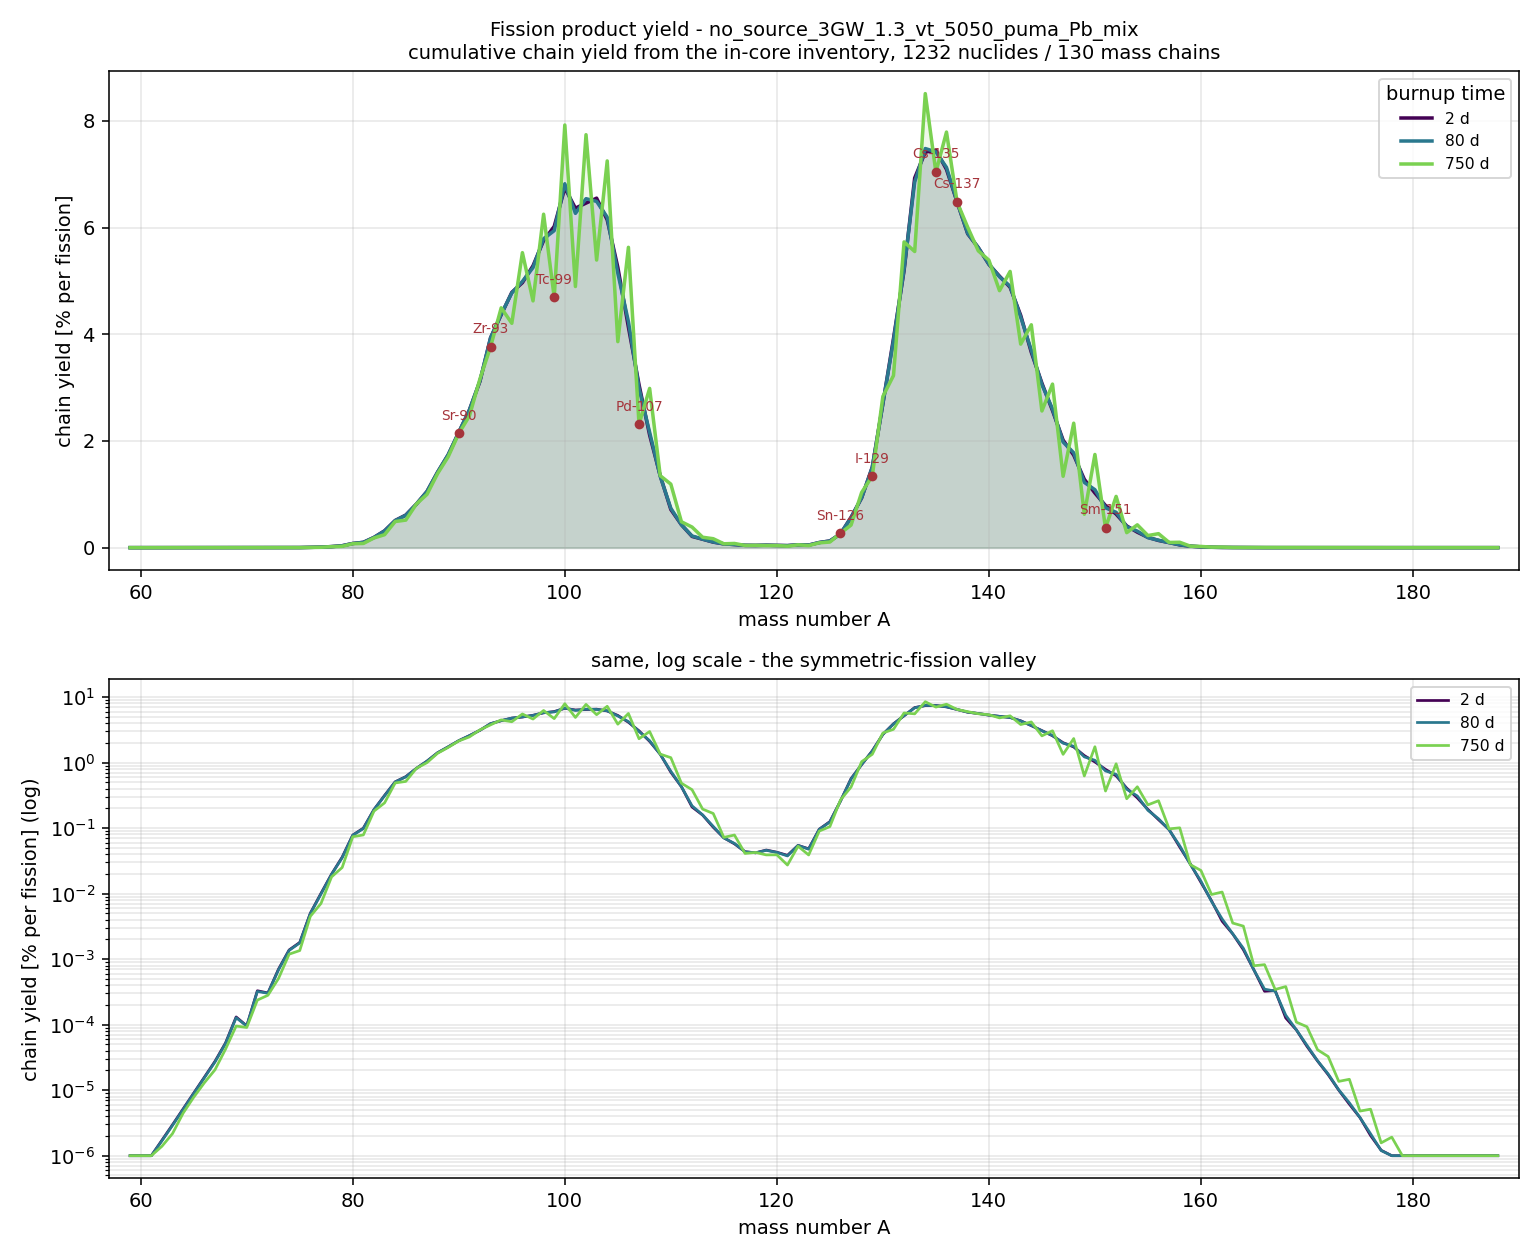
\includegraphics[width=0.9\textwidth]{figures/case4_puma_recycle_100yr_fp_yield}
  \caption[Fission-product yield of the \(50/50\) core.]{Cumulative fission-product
  chain yield of the \(50/50\) plutonium-minor-actinide core (ADS~2). Relative to
  the minor-actinide-only core, the plutonium-bearing feed fills in the
  symmetric-fission valley and shifts the light peak slightly higher in mass, the
  expected signature of a heavier fissioning system.}
  \label{fig:results-case4-recycle-fpyield}
\end{figure}

The per-cycle mass accounting is summarized by the burn fraction, the ratio of
actinide mass destroyed to actinide mass charged. For the minor-actinide-only
core this fraction is constant at \(41.3\%\) across every cycle
(Figure~\ref{fig:results-case3-recycle-percycle}), a direct consequence of the
reduced-order model: each core is irradiated to the same point on the same
depletion trajectory, so each cycle removes the same fraction of its charge. For
the \(50/50\) core the burn fraction rises to just under \(50\%\)
(Figure~\ref{fig:results-case4-recycle-percycle}); the plutonium half of that feed
fissions more readily than the minor-actinide vector, so a larger fraction of each
charge is consumed per pass.

The burn fraction reported here is the net reduction in total actinide mass,
calculated from the \texttt{ActinideDestroyed} event according to
Equation~\ref{eq:ads-destroyed}. Equation~\ref{eq:ads-ratio} first determines the
mass retained in the discharged product, after which the archetype subtracts the
total actinide mass remaining in that product from the total actinide mass in the
matched case's initial loading. Because plutonium is included in the total
actinide inventory, minor actinides converted into plutonium remain in
\(M_{\mathrm{out}}a_c(t_{\mathrm{irr}})\) and are not counted as destroyed. The
reported value therefore represents net actinide destruction in the tracked
depletion inventory, rather than the disappearance of minor actinides alone.

This per-cycle rate can be checked against first principles. Fissioning one
kilogram of actinide releases approximately \(0.93~\mathrm{GW\text{-}d}\) of
thermal energy, so a \(3000~\mathrm{MW_{th}}\) core destroys about
\(3.2~\mathrm{kg}\) of actinide per full-power day, or roughly
\(1{,}120~\mathrm{kg\,yr^{-1}}\) at full power. Applied to the ten-year
minor-actinide cycle, this predicts a per-cycle destruction close to the
\(11{,}150~\mathrm{kg}\) read from the \textsc{Serpent} case, agreeing to within a
few percent. The reduced-order transmutation model is therefore consistent with
the fission energy balance, an independent validation of the archetype's mass
accounting.

\begin{figure}[htbp]
  \centering
  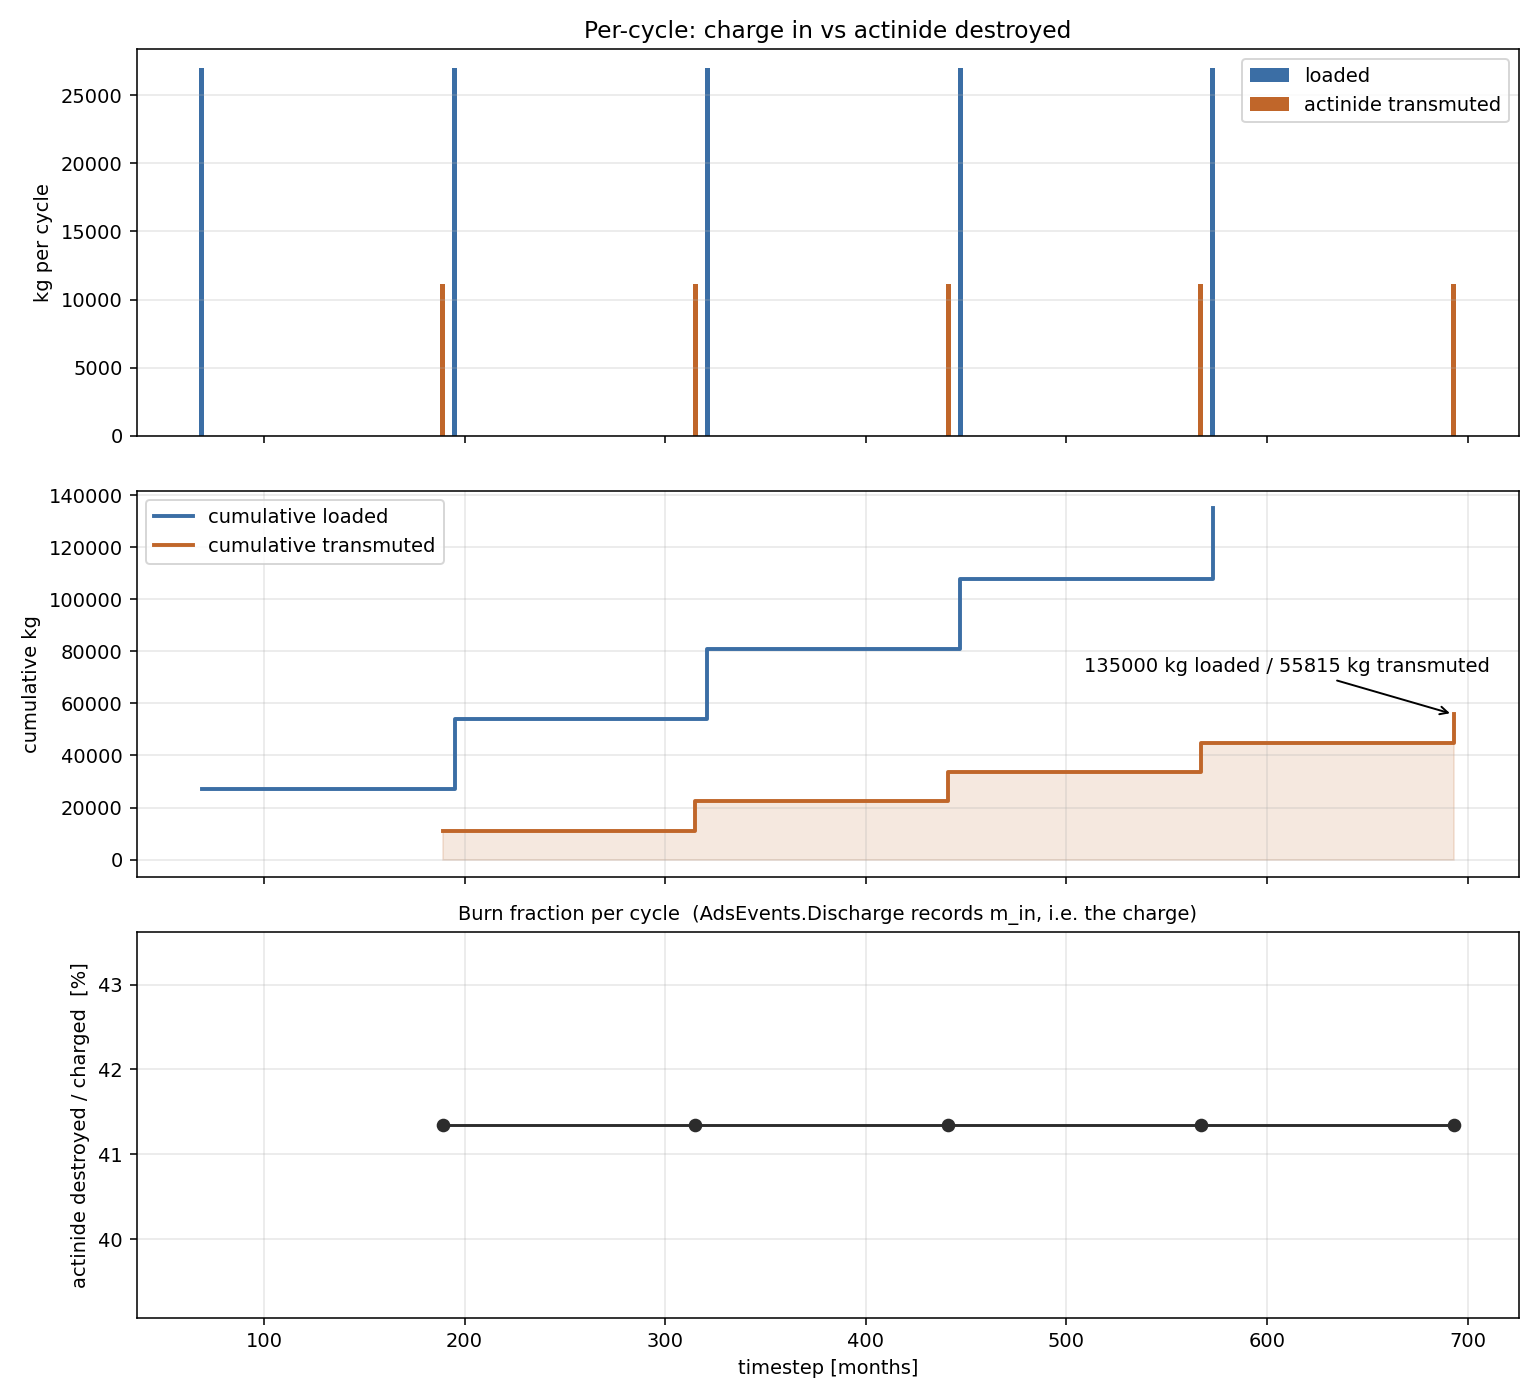
\includegraphics[width=0.95\textwidth]{figures/case3_ma_recycle_100yr_percycle}
  \caption[Per-cycle mass accounting for the minor-actinide-only core.]{Per-cycle
  charge and actinide destruction for the minor-actinide-only core (ADS~1),
  100-year recycling run. Each cycle charges \(27~\mathrm{t}\) and records
  \(11.15~\mathrm{t}\) of net actinide destruction, a constant burn fraction of \(41.3\%\) (bottom panel). The
  cumulative panel (centre) reaches \(135~\mathrm{t}\) charged and
  \(55.8~\mathrm{t}\) of cumulative net actinide destruction over five cycles.}
  \label{fig:results-case3-recycle-percycle}
\end{figure}

\begin{figure}[htbp]
  \centering
  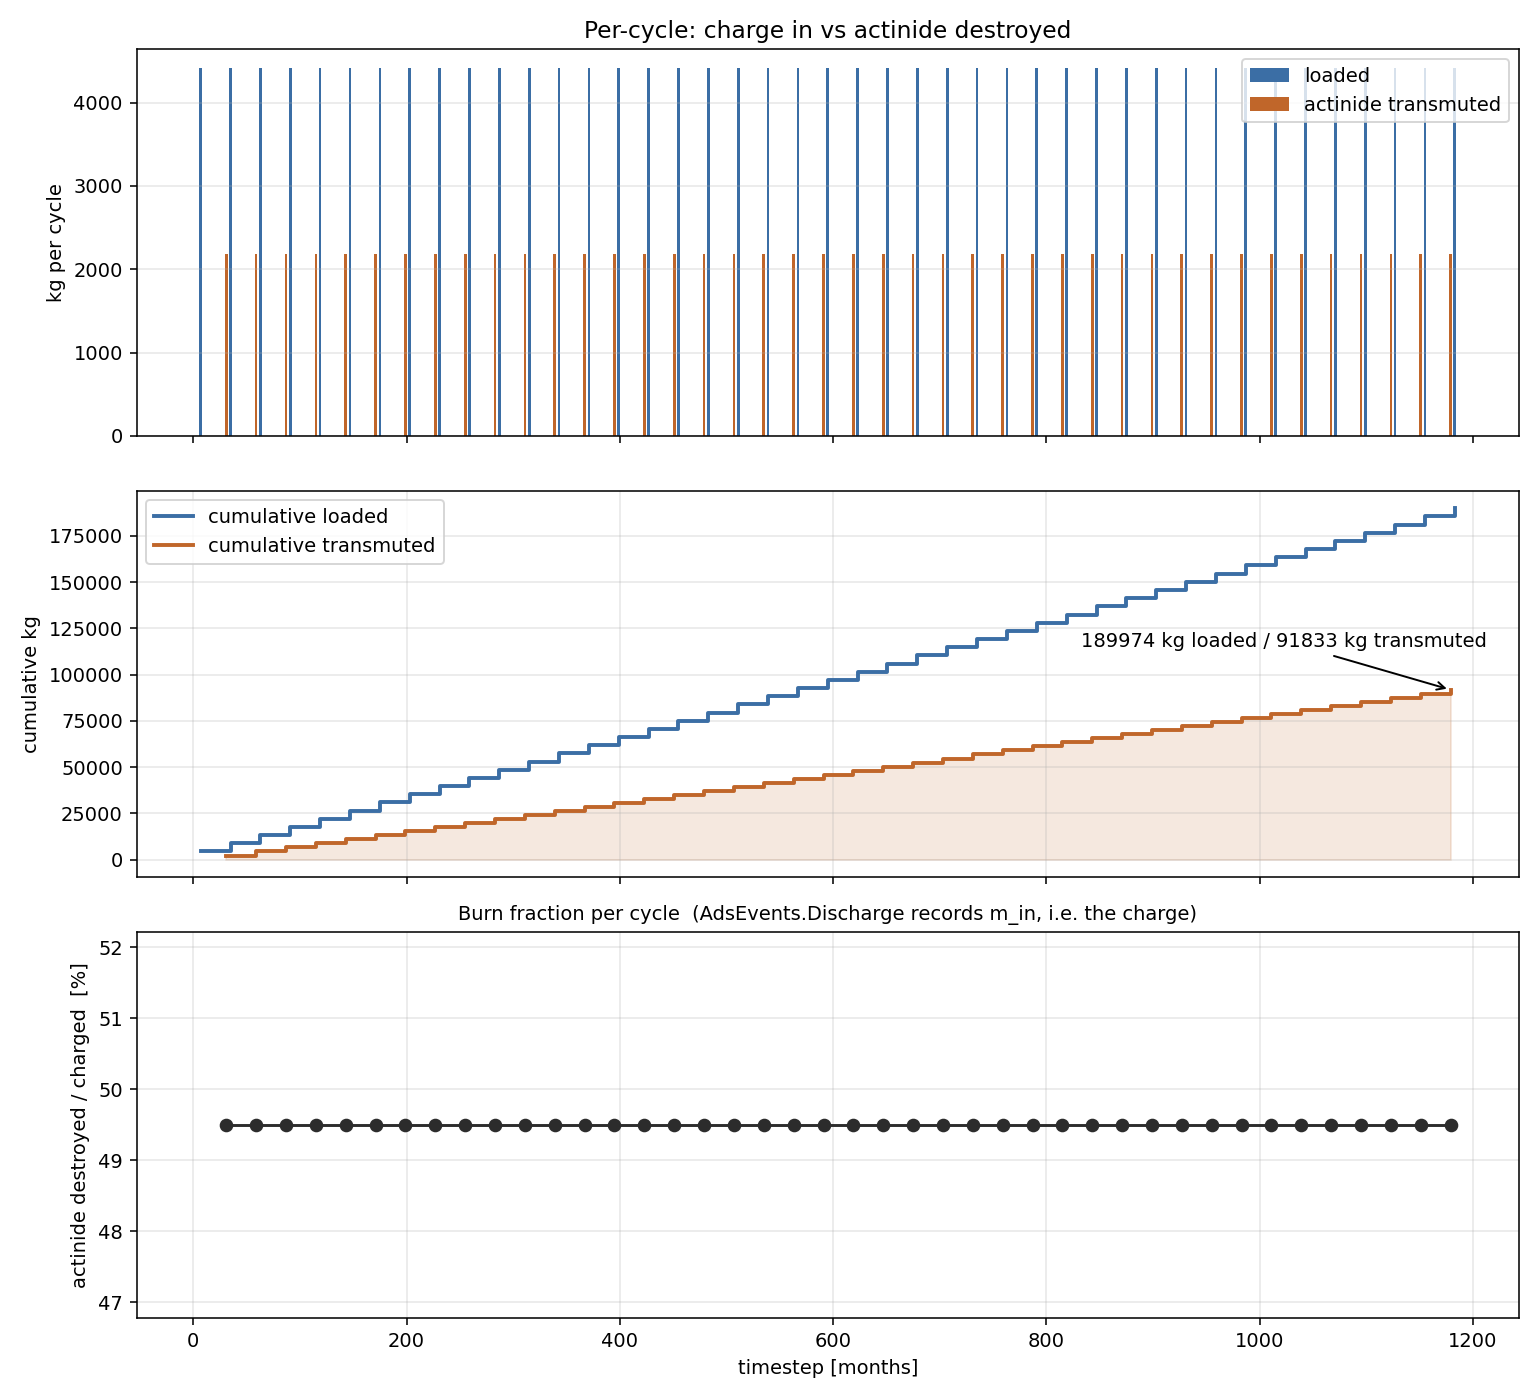
\includegraphics[width=0.95\textwidth]{figures/case4_puma_recycle_100yr_percycle}
  \caption[Per-cycle mass accounting for the \(50/50\) core.]{Per-cycle charge and
  actinide destruction for the \(50/50\) plutonium-minor-actinide core (ADS~2),
  100-year recycling run. Each cycle charges \(4.4~\mathrm{t}\) and records
  \(2.2~\mathrm{t}\) of net actinide destruction, a burn fraction just under \(50\%\). The small, fast-cycling
  core completes 42 cycles over the horizon.}
  \label{fig:results-case4-recycle-percycle}
\end{figure}

\subsection{Core Size and Feed Composition: the Two Burner Cases}
\label{subsec:results-ads-cases}

The two burner configurations produce very different operating histories, driven
entirely by core size and the resulting cycle length.
Figures~\ref{fig:results-case3-recycle-dutycycle}
and~\ref{fig:results-case4-recycle-dutycycle} show the core state, irradiating or
idle, over the 100-year horizon for the two cases.

The minor-actinide-only core is large (\(27~\mathrm{t}\)) and is irradiated for
ten years per cycle. Over 100 years of recycling it completes only five cycles and
then falls idle for the remainder of the horizon, reaching a duty factor of
\(50\%\). The core stops not because the horizon ends, but because the quantity
of recoverable neptunium, americium, and curium accumulated in its feed buffer no
longer reaches the \(27~\mathrm{t}\) full-core loading required by the archetype.
This does not mean that no actinide remains in the fuel cycle: some surviving
actinide has been converted to plutonium, which is not returned to the
minor-actinide-only feed, while additional material remains in discharged
products, waste, and facility buffers. The \(50/50\) core, by contrast, is small
(\(4.4~\mathrm{t}\)) and is cycled every two years. It completes 42 cycles and
runs essentially continuously across the full horizon, at a duty factor of
\(85\%\). It never exhausts its feed because it consumes minor actinide slowly and
supplements it with the far more abundant plutonium.

This is the central distinction between the two configurations. The
minor-actinide-only core is \emph{feed-limited}: its throughput is set by how much
minor actinide the inventory can supply, not by reactor physics. The \(50/50\)
core is \emph{cycle-limited}: it processes feed as fast as its cycle allows, and
the inventory is deep enough, because it draws on plutonium, to sustain that pace
for a century. The trade-off is that the \(50/50\) core is no longer a pure
minor-actinide burner: half of what it destroys is plutonium, so it addresses the
broader transuranic inventory rather than the minor actinides specifically. Over
the full horizon it destroys \(91.8~\mathrm{t}\) of actinide against the
minor-actinide core's \(55.8~\mathrm{t}\), but that larger figure is achieved by
co-burning plutonium the minor-actinide case leaves untouched.

\begin{figure}[htbp]
  \centering
  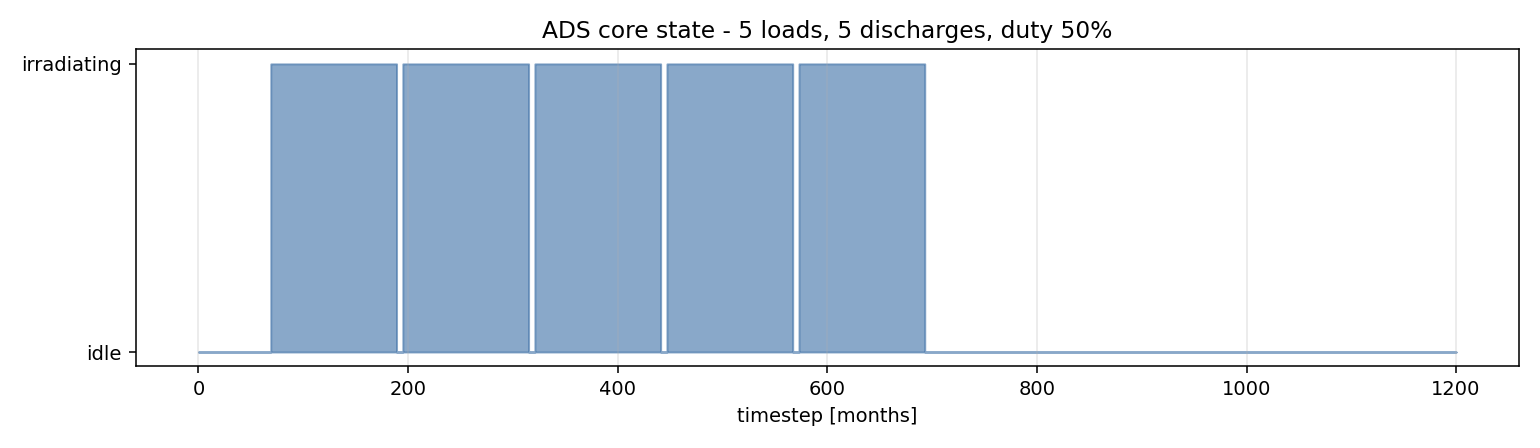
\includegraphics[width=0.95\textwidth]{figures/case3_ma_recycle_100yr_dutycycle}
  \caption[Core state of the minor-actinide-only burner.]{Irradiating-or-idle
  state of the minor-actinide-only core (ADS~1) over the 100-year recycling run.
  The core completes five ten-year cycles and then falls idle because its
  recoverable Np-Am-Cm feed no longer reaches the \(27~\mathrm{t}\) full-core
  loading threshold; the duty factor is \(50\%\).}
  \label{fig:results-case3-recycle-dutycycle}
\end{figure}

\begin{figure}[htbp]
  \centering
  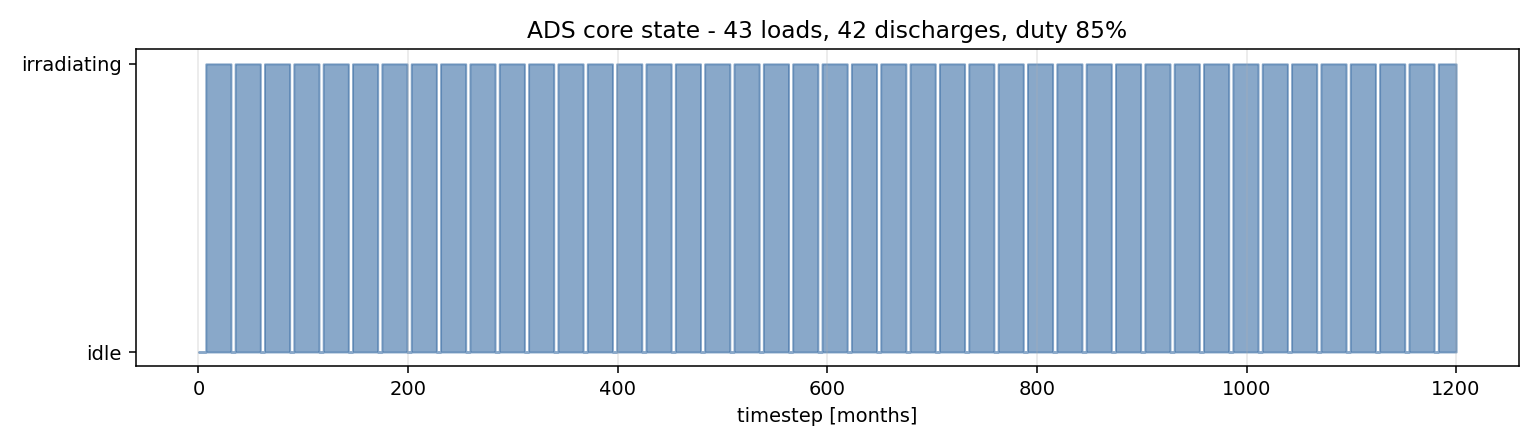
\includegraphics[width=0.95\textwidth]{figures/case4_puma_recycle_100yr_dutycycle}
  \caption[Core state of the \(50/50\) burner.]{Irradiating-or-idle state of the
  \(50/50\) core (ADS~2) over the 100-year recycling run. The small, fast-cycling
  core runs essentially continuously at a duty factor of \(85\%\), sustained by
  the plutonium fraction of its feed.}
  \label{fig:results-case4-recycle-dutycycle}
\end{figure}

For the \(50/50\) core the once-through and recycling runs are indistinguishable,
because the core is cycle-limited: within each two-year cycle there is little
surviving actinide to recover before the next core is due, so recycling changes
almost nothing. This confirms the cycle-limited regime and is why only a single
\(50/50\) run is shown.

\subsection{Recycling versus Once-Through for the Minor-Actinide Core}
\label{subsec:results-ads-recycle}

The minor-actinide-only core is the one configuration where recycling materially
changes the outcome, precisely because it is feed-limited. Comparing the recycling
per-cycle history (Figure~\ref{fig:results-case3-recycle-percycle}) with the
once-through history (Figure~\ref{fig:results-case3-oncethrough-percycle}) isolates
the effect. The two runs share an identical per-cycle signature, the same
\(27~\mathrm{t}\) charge, the same \(11.15~\mathrm{t}\) destroyed, and the same
\(41.3\%\) burn fraction in the bottom panel of each figure, because the reduced-
order depletion physics does not depend on where the feed came from. What differs
is how many cycles the burner completes before its feed is spent: three under
once-through, five under recycling.

The cumulative panels make the consequence concrete. In once-through mode the burner charges \(81~\mathrm{t}\) in total and
records \(33.5~\mathrm{t}\) of net actinide destruction; with recycling it
charges \(135~\mathrm{t}\) and records \(55.8~\mathrm{t}\), an
increase of \(1.67\times\) in actinide destroyed. Recycling achieves this by
recovering the surviving minor actinides from each discharge and returning them to
the feed, so the same atoms make more than one pass through the core and the
burner sustains operation past the point where the once-through supply is spent.

The charged figure is itself the clearest evidence of reuse. The total accessible
minor-actinide inventory is only \(103.8~\mathrm{t}\)
(Section~\ref{sec:results-baseline}), yet the recycling run charges
\(135~\mathrm{t}\), more minor actinide than exists in the national inventory.
This is possible only because recycling returns material for additional passes;
the excess of roughly \(31~\mathrm{t}\) is minor actinide irradiated more than
once. The once-through run, by contrast, charges \(81~\mathrm{t}\), comfortably
within the inventory, and simply stops when the accessible feed is gone.

Even with recycling, however, the burner still stops well short of the horizon.
The initial \(103.8~\mathrm{t}\) minor-actinide inventory is only about
\(3.8\) fresh core-loadings. After each irradiation, only the surviving
neptunium, americium, and curium is eligible to return to the ADS~1 feed; actinide
converted to plutonium is routed outside that feed stream, and the archetype will
not load a partial core. Recycling therefore extends the campaign from three
cores to five, but eventually the recoverable minor-actinide feed remains below
the \(27~\mathrm{t}\) loading threshold.

\begin{figure}[htbp]
  \centering
  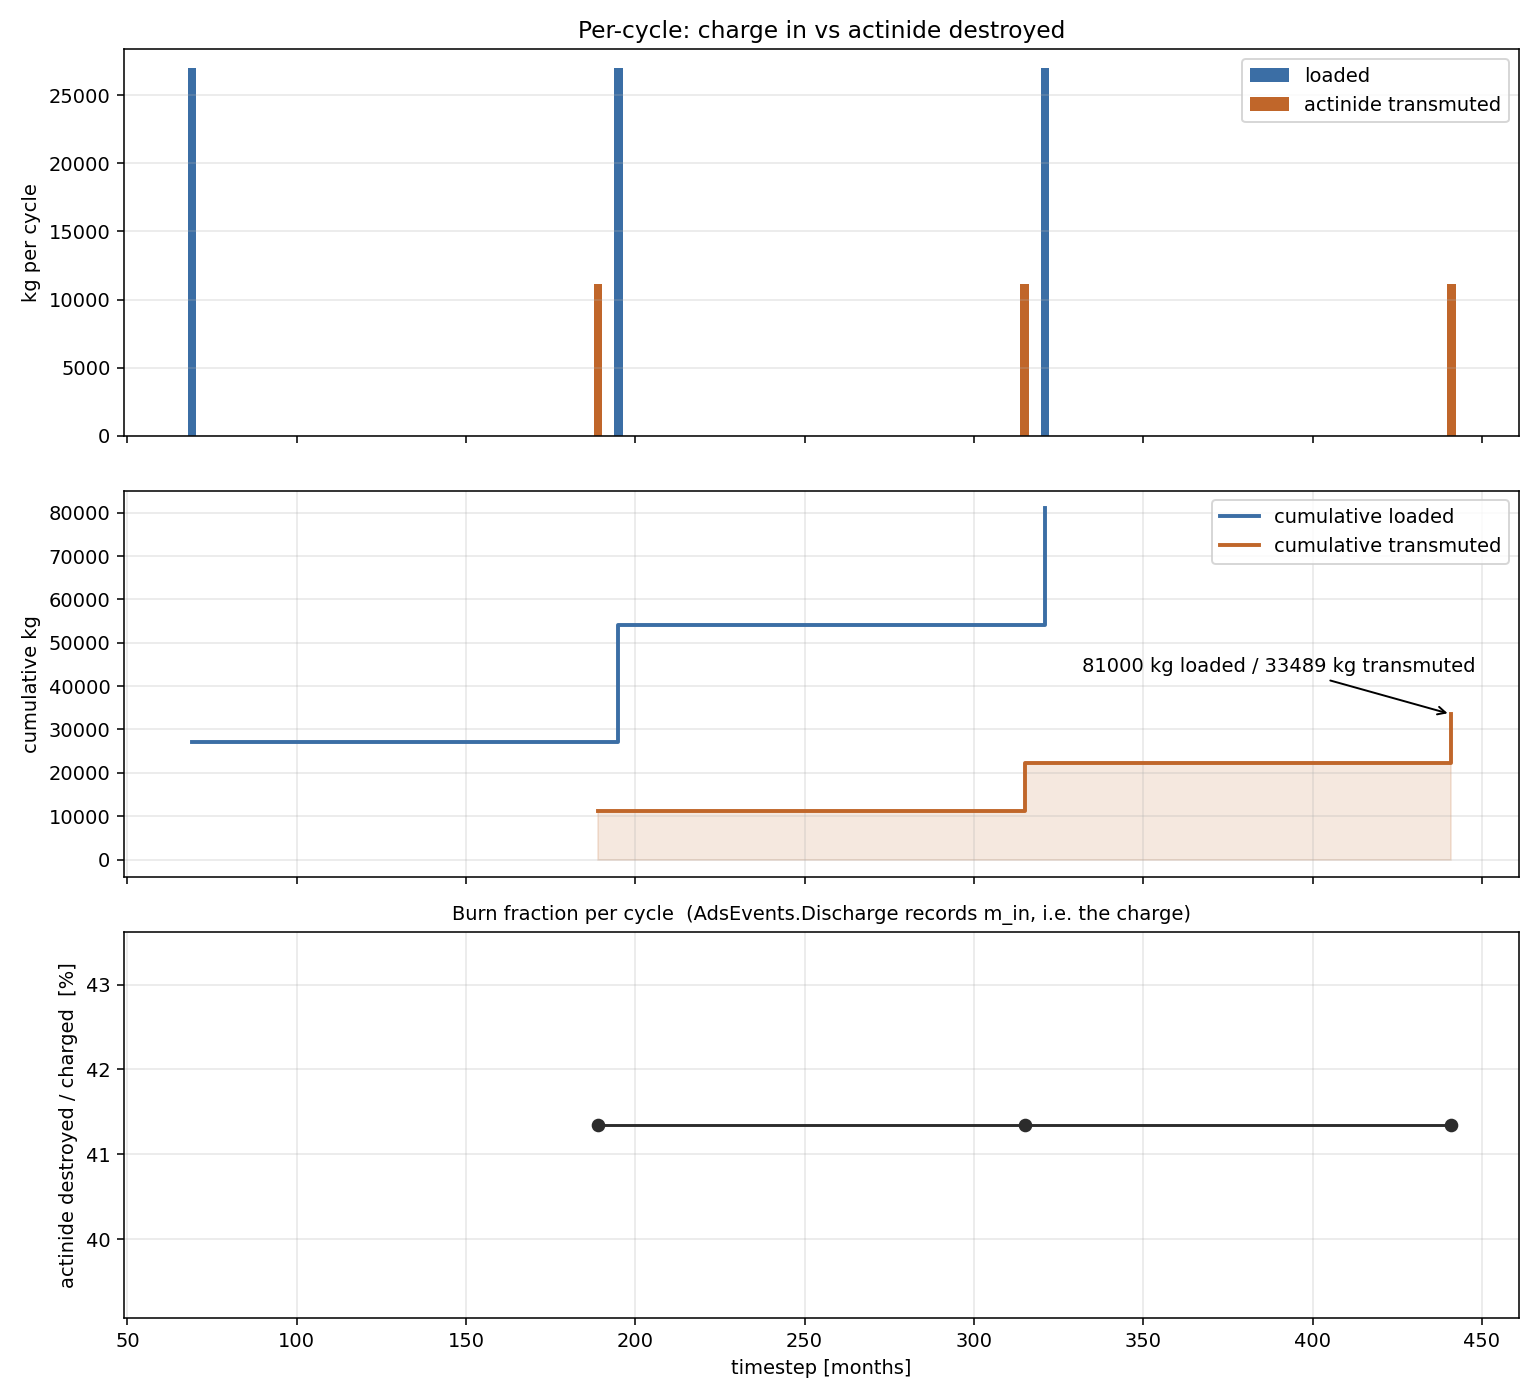
\includegraphics[width=0.95\textwidth]{figures/case3_ma_oncethrough_100yr_percycle}
  \caption[Per-cycle mass accounting for the minor-actinide-only core,
  once-through.]{Per-cycle charge and actinide destruction for the
  minor-actinide-only core (ADS~1), 100-year once-through run. The per-cycle
  charge, destruction, and \(41.3\%\) burn fraction match the recycling run
  (Figure~\ref{fig:results-case3-recycle-percycle}), but the burner completes only
  three cycles, reaching \(81~\mathrm{t}\) charged and \(33.5~\mathrm{t}\)
  of cumulative net actinide destruction before its feed is exhausted.}
  \label{fig:results-case3-oncethrough-percycle}
\end{figure}

\subsection{Transmutation Rate and Mission Scale}
\label{subsec:results-ads-rate}

Taken together, these results frame the scale of the transmutation mission. A
single \(3000~\mathrm{MW_{th}}\) unit destroys actinide at up to about
\(1{,}120~\mathrm{kg\,yr^{-1}}\) at full power, reduced in proportion to its duty
factor. Over a 30-year mission the \(50/50\) core, running near-continuously,
destroys on the order of \(27~\mathrm{t}\) of actinide per unit, while the
minor-actinide-only core destroys less because it stalls once its feed is spent.
The two horizons reinforce this: a cycle-limited core scales its output roughly
linearly with the length of the mission, whereas a feed-limited core plateaus once
the accessible inventory is consumed, which is why extending the minor-actinide
core from 30 to 100 years adds only two further cycles.

The consequence is that sizing a fleet to destroy the minor-actinide inventory is
not the usual reactor-capacity problem. The entire national minor-actinide
inventory is under four core-loadings; the limitation is how quickly that finite
inventory can be retrieved, separated, and, critically, recycled, not how much
reactor power is installed. Additional units shorten the calendar time to work
through the available feed but cannot destroy more minor actinide than the
inventory contains. A configuration that instead co-burns plutonium, as the
\(50/50\) core does, sidesteps the feed limit but redefines the mission from
minor-actinide destruction to bulk transuranic destruction. This inversion of the
usual sizing question, feed-bound rather than power-bound, is the central
practical finding of the transmutation results, and it is examined further in the
discussion of Section~\ref{sec:results-discussion}.


%%%%%%%%%%%%%%%%%%%%%%%%%%%%%%%%%%%%%%%%%%%%%%%%%%%%%%%%%%%%%%%%%%%%%%%%%%%%%%%%%%%%%%%%%%%%%%%%%%%%%%%%%%%%%%%%%%%%%%%%%%%%%%%%%
%%%%%%%%%%%%%%%%%%%%%%%%%%%%%%%%%%%%%%%%%%%%%%%%%%%%%%%%%%%%%%%%%%%%%%%%%%%%%%%%%%%%%%%%%%%%%%%%%%%%%%%%%%%%%%%%%%%%%%%%%%%%%%%%%
%%%%%%%%%%%%%%%%%%%%%%%%%%%%%%%%%%%%%%%%%%%%%%%%%%%%%%%%%%%%%%%%%%%%%%%%%%%%%%%%%%%%%%%%%%%%%%%%%%%%%%%%%%%%%%%%%%%%%%%%%%%%%%%%%

\section{Processed Inventory}
\label{sec:results-evolution}

The transmutation results of Section~\ref{sec:results-ads} describe what the
burner does per cycle; this section follows the material through the whole fuel
cycle and asks what becomes of the national inventory once it is processed. Every
kilogram drawn from \texttt{us\_inventory} meets one of three fates: it is
destroyed by fission in the \gls{ADS}, it is recovered and returned to the feed
under recycling, or it is routed to disposal. Tracking these streams shows both
what the mission accomplishes and what it leaves behind, and connects the results
back to the waste-management motivation of Chapter~\ref{ch:background}.

\subsection{Disposition of the Minor-Actinide Inventory}
\label{subsec:results-fate-ma}

Table~\ref{tab:results-ma-fate} closes the actinide mass balance against the
\(103.8~\mathrm{t}\) of minor actinide initially present in the accessible
inventory (Section~\ref{sec:results-baseline}). The quantity labeled
``undestroyed descendant actinide'' is the initial actinide mass minus the net
actinide destruction recorded by the ADS. It is therefore not equivalent to
minor-actinide feed still available to the burner: it includes any surviving
neptunium, americium, and curium, actinides produced by transmutation such as
plutonium, material routed to waste, and material held in facility buffers.

In once-through operation the burner records \(33.5~\mathrm{t}\) of net actinide
destruction and leaves \(70.3~\mathrm{t}\) of descendant actinide undestroyed. Of
that remainder, roughly \(47.5~\mathrm{t}\) is surviving actinide discharged to
waste, while about \(22.8~\mathrm{t}\) remains in unprocessed inventory because
it is insufficient to form another \(27~\mathrm{t}\) core.

With recycling, net actinide destruction increases to \(55.8~\mathrm{t}\), leaving
\(48.0~\mathrm{t}\) of descendant actinide somewhere in the modeled fuel cycle.
The \(48.0~\mathrm{t}\) value does not imply that a further \(27~\mathrm{t}\)
minor-actinide core could be loaded. In the ADS~1 flowsheet, only Np, Am, and Cm
are recovered as burner feed; plutonium produced during irradiation is routed
outside the minor-actinide feed stream, and the remaining recoverable
minor-actinide inventory is distributed among products and buffers. The ADS
therefore stalls when its feed buffer cannot again accumulate a full
\(27~\mathrm{t}\) loading.

\begin{table}[htbp]
    \centering
    \caption{Actinide mass balance relative to the \(103.8~\mathrm{t}\) of minor
    actinide initially present in the accessible inventory at the end of the
    100-year minor-actinide-only runs. ``Undestroyed descendant actinide''
    includes surviving minor actinides, actinides produced by transmutation,
    material routed to waste, and material held in facility buffers; it is not
    the mass of usable minor-actinide feed remaining.}
    \label{tab:results-ma-fate}
    \begin{tabular}{p{0.42\textwidth} p{0.22\textwidth} p{0.22\textwidth}}
        \hline
        \textbf{Disposition} & \textbf{Once-through} & \textbf{Recycle} \\
        \hline
        Net actinide destruction          & \(33.5~\mathrm{t}\) & \(55.8~\mathrm{t}\) \\
        Undestroyed descendant actinide     & \(70.3~\mathrm{t}\) & \(48.0~\mathrm{t}\) \\
        \hline
        Initial accessible MA inventory     & \(103.8~\mathrm{t}\) & \(103.8~\mathrm{t}\) \\
        \hline
    \end{tabular}
\end{table}

\subsection{Composition of the Waste Stream}
\label{subsec:results-fate-waste}

Figure~\ref{fig:results-case3-recycle-waste} shows the final composition of the
waste repository for the minor-actinide-only recycling run, as the mass of each of
the 25 most abundant nuclides. The stream is overwhelmingly uranium: \({}^{238}\mathrm{U}\)
alone accounts for roughly \(8.5\times10^{4}~\mathrm{t}\), four orders of magnitude
above any minor actinide. This is a direct consequence of the scarcity documented
in Section~\ref{sec:results-baseline}. Because minor actinide is only about
\(0.12\%\) of the spent fuel, extracting the roughly \(100~\mathrm{t}\) the burner
consumes requires separations to process on the order of the entire drawn
inventory, tens of thousands of tonnes of spent fuel, and the uranium and fission
products stripped from that fuel dominate the disposal stream. The mass sent to
disposal is therefore not reduced by the transmutation mission; it is only changed
in character.

That change in character is nonetheless the intended effect, and it is visible in
the figure. Minor actinides are almost absent from the waste: americium, the most
abundant minor actinide in the original fuel, does not appear among the major
waste nuclides at all under recycling, having been recovered and burned. In the
once-through run the same plot shows a small residual \({}^{241}\mathrm{Am}\) peak,
which recycling removes, a direct illustration of recovery closing that pathway.
The minor-actinide-only cycle thus succeeds in stripping minor actinide from the
waste, but does not reduce its volume.

The figure also exposes the principal limitation of the minor-actinide-only
configuration. Plutonium is the second-largest component of the waste, with
\({}^{239}\mathrm{Pu}\) near \(7\times10^{2}~\mathrm{t}\): because this burner
consumes only minor actinide, separations routes the entire plutonium content of
every processed assembly straight to disposal, untouched. A cycle designed to
destroy minor actinide therefore leaves the larger and equally long-lived
plutonium inventory in the waste, which is precisely the gap the \(50/50\)
configuration is meant to address.

\begin{figure}[htbp]
  \centering
  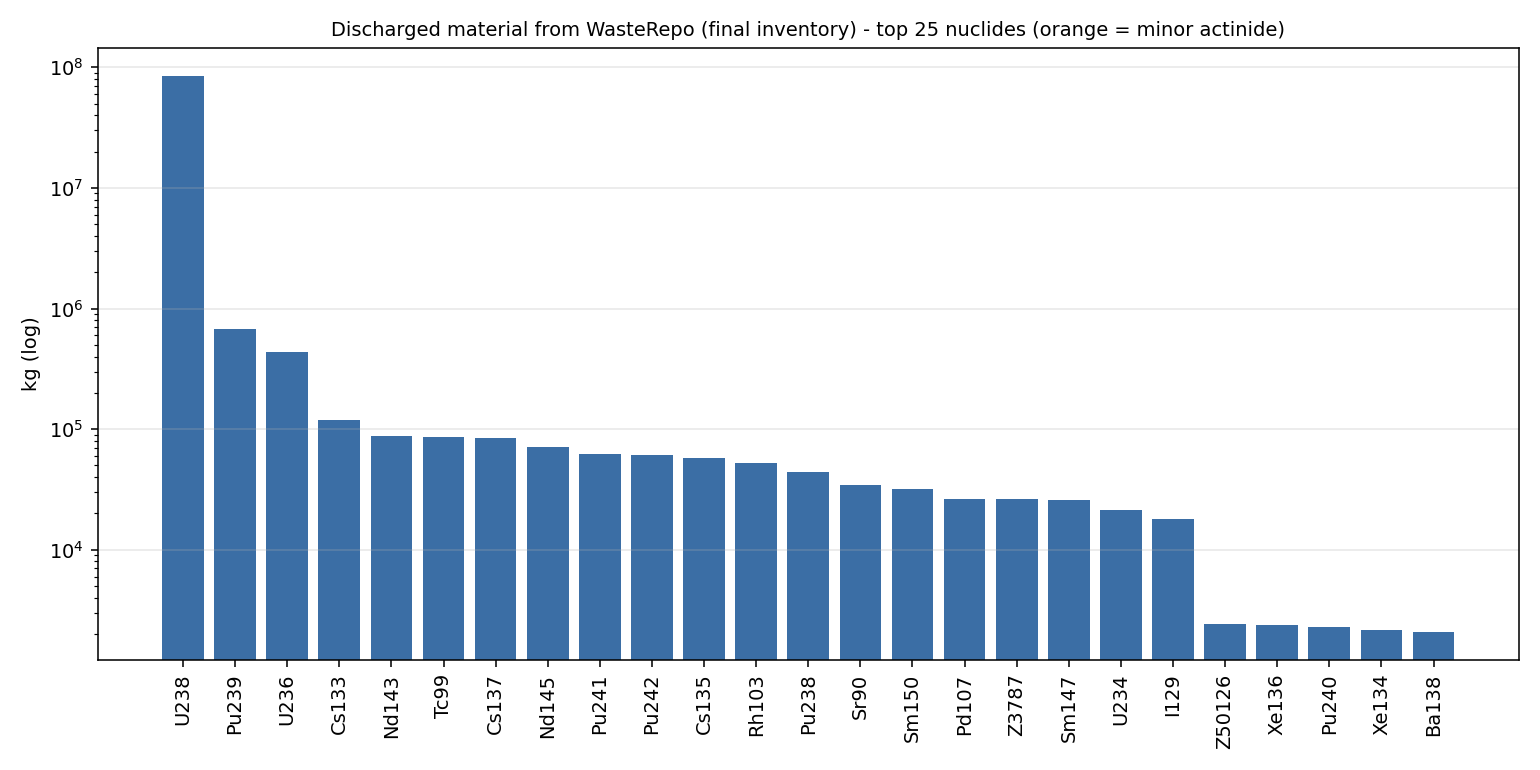
\includegraphics[width=0.95\textwidth]{figures/case3_ma_recycle_100yr_waste_composition}
  \caption[Waste-stream composition for the minor-actinide-only core.]{Final
  waste-repository composition for the minor-actinide-only recycling run (ADS~1),
  showing the 25 most abundant nuclides on a logarithmic mass scale; minor
  actinides are highlighted. The stream is dominated by uranium and plutonium
  stripped by separations, while minor actinides are nearly absent, having been
  recovered and burned.}
  \label{fig:results-case3-recycle-waste}
\end{figure}

\subsection{Material Recovered under Recycling}
\label{subsec:results-fate-recovered}

Where the minor-actinide-only cycle sends plutonium to waste, the \(50/50\)
configuration returns it to the feed. Figure~\ref{fig:results-case4-recycle-product}
shows the material discharged from the \gls{ADS} in the \(50/50\) recycling run,
which separations recovers and blends back into fresh feed. The stream is led by
plutonium isotopes, surviving and bred \({}^{239}\mathrm{Pu}\),
\({}^{238}\mathrm{Pu}\), and \({}^{240}\mathrm{Pu}\), followed by the minor
actinides \({}^{237}\mathrm{Np}\), \({}^{244}\mathrm{Cm}\), \({}^{241}\mathrm{Am}\),
and their heavier companions, alongside the fission products of the cycle. By
recovering the plutonium as well as the minor actinides, the \(50/50\) cycle keeps
that plutonium in the burner over successive passes rather than stranding it in
waste, which is why it addresses the broader transuranic inventory rather than the
minor actinides alone. The presence of \({}^{242\mathrm{m}}\mathrm{Am}\) in the
recovered stream also confirms that the archetype preserves the metastable state
through the composition transformation, rather than collapsing it onto the ground
state.

\begin{figure}[htbp]
  \centering
  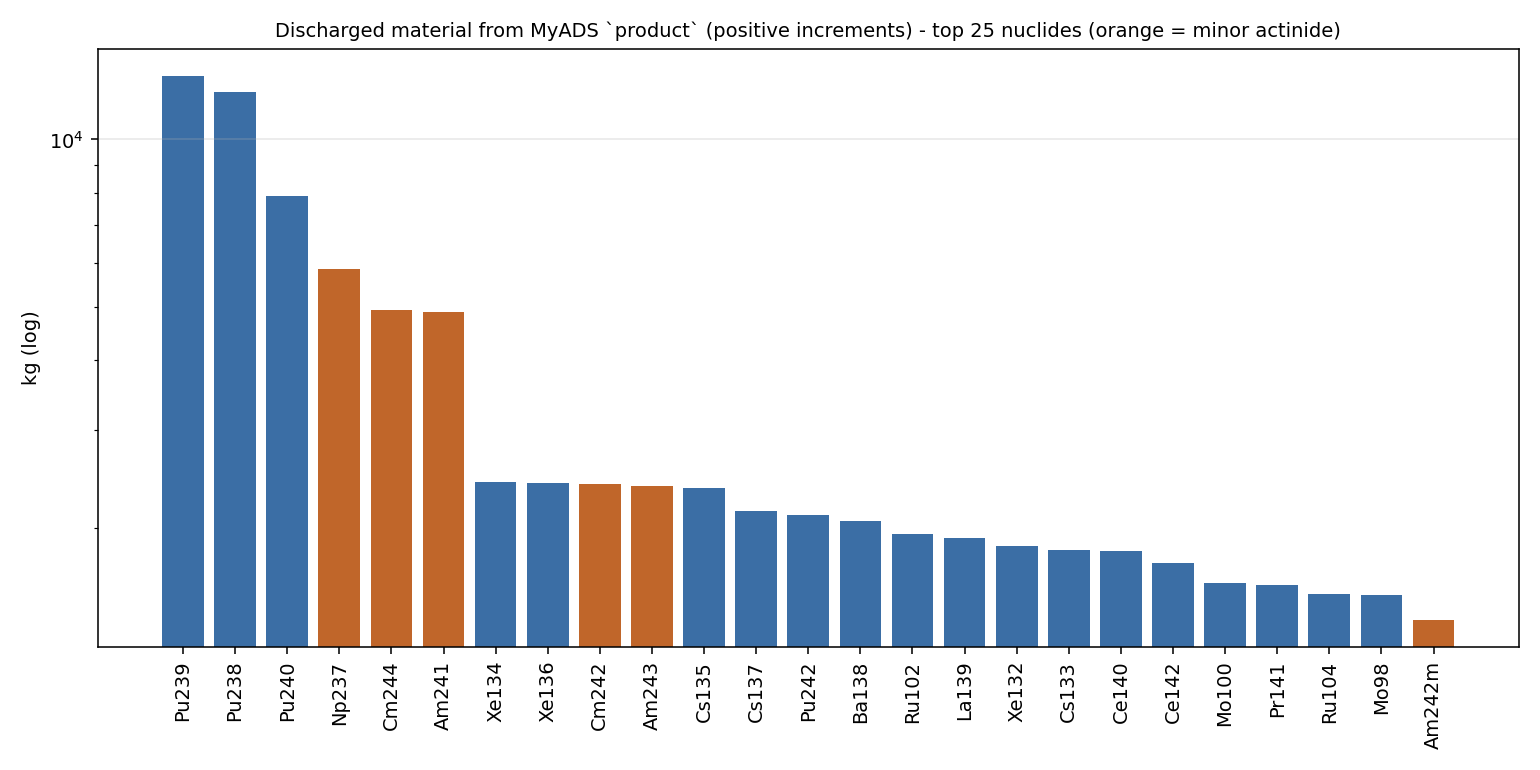
\includegraphics[width=0.95\textwidth]{figures/case4_puma_recycle_100yr_ads_product}
  \caption[Recovered discharge stream for the \(50/50\) core.]{Composition of the
  material discharged from the \gls{ADS} in the \(50/50\) recycling run (ADS~2),
  showing the 25 most abundant nuclides on a logarithmic mass scale; minor
  actinides are highlighted. Plutonium leads the recovered stream, followed by the
  minor actinides and fission products, all of which recycling returns to the
  feed.}
  \label{fig:results-case4-recycle-product}
\end{figure}

\subsection{Implications for the Waste Inventory}
\label{subsec:results-fate-implications}

Taken together, these results qualify what transmutation achieves for the national
inventory. Over a century, even the more favorable recycling configuration
destroys only about half of the accessible minor actinide, and it does so at the
cost of processing essentially the entire spent-fuel inventory, the bulk of which, 
uranium, fission products, and, for the minor-actinide-only cycle, plutonium, 
still requires disposal. The mission changes the isotopic character of the waste
by removing minor actinide, which is the component that dominates its long-term
radiotoxicity and heat load; it does not substantially reduce the bulk material mass requiring management
and disposal. Quantifying the resulting reduction in radiotoxicity or decay heat
would require coupling these mass histories to a decay and dose calculation, which
is beyond the scope of this work but is a natural extension of it
(Chapter~\ref{ch:conclusion}). What the fuel-cycle results establish is the
upstream reality any such benefit must be weighed against: minor-actinide
transmutation is constrained not by reactor performance but by the scarcity of its
feed and the scale of the inventory that must be handled to extract it.


%%%%%%%%%%%%%%%%%%%%%%%%%%%%%%%%%%%%%%%%%%%%%%%%%%%%%%%%%%%%%%%%%%%%%%%%%%%%%%%%%%%%%%%%%%%%%%%%%%%%%%%%%%%%%%%%%%%%%%%%%%%%%%%%%
%%%%%%%%%%%%%%%%%%%%%%%%%%%%%%%%%%%%%%%%%%%%%%%%%%%%%%%%%%%%%%%%%%%%%%%%%%%%%%%%%%%%%%%%%%%%%%%%%%%%%%%%%%%%%%%%%%%%%%%%%%%%%%%%%
%%%%%%%%%%%%%%%%%%%%%%%%%%%%%%%%%%%%%%%%%%%%%%%%%%%%%%%%%%%%%%%%%%%%%%%%%%%%%%%%%%%%%%%%%%%%%%%%%%%%%%%%%%%%%%%%%%%%%%%%%%%%%%%%%

\section{Discussion}
\label{sec:results-discussion}

The results of this chapter can be read as a single argument about scale. The
\texttt{us\_inventory} and \texttt{ads} archetypes were built to connect a
detailed, assembly-resolved picture of the U.S. spent-fuel inventory to a
reduced-order model of an accelerator-driven burner, and running them together
turns qualitative expectations about minor-actinide transmutation into quantified
constraints. Two findings dominate, and both point the same way.

\subsection{The Mission is Feed-Bound}
\label{subsec:discussion-feedbound}

The central result is that a minor-actinide transmutation mission is limited by
the availability of its feed rather than by installed reactor capacity. The
accessible minor-actinide inventory is \(103.8~\mathrm{t}\), under four loadings
of a single \(27~\mathrm{t}\) core, so the binding question is not how much power
can be deployed but how quickly that finite, dilute inventory can be retrieved,
separated, and recycled. The minor-actinide-only core makes this concrete: it is
feed-limited, stalling after three cores once-through or five with recycling
(Section~\ref{subsec:results-ads-recycle}), and no increase in reactor power can
change that, because the feed to sustain further cores does not exist. This
inverts the usual framing of a reactor deployment, in which capacity is the
constraint and fuel is assumed abundant.

A simple rate calculation frames the fleet question that follows from this. A
\(3000~\mathrm{MW_{th}}\) unit destroys actinide at up to about
\(1{,}120~\mathrm{kg\,yr^{-1}}\) at full power
(Section~\ref{subsec:results-ads-rate}), so clearing the \(103.8~\mathrm{t}\)
inventory represents on the order of \(90\) unit-years of full-power operation.
Distributed over a 30-year mission this is roughly three units' worth of
destruction capacity; a single unit would require most of a century, and the
feed-limited minor-actinide core cannot in practice run at full duty for that long.
This is not a precise fleet-sizing, it omits reprocessing losses, retrieval and
transport logistics, and the duty-factor penalty the feed limit itself imposes, but
it establishes the order of magnitude: the transmutation of the national
minor-actinide inventory is a task for a handful of high-power units over decades,
and its pace is set by fuel handling rather than by how many units are built.

The \(50/50\) configuration escapes the feed limit, but only by changing the
mission. By co-burning plutonium, ten times more abundant in the inventory than
minor actinide, the small, fast-cycling core stays fed for the full century at a
\(85\%\) duty factor and destroys \(91.8~\mathrm{t}\) of actinide, far more than the
minor-actinide core's \(55.8~\mathrm{t}\)
(Section~\ref{subsec:results-ads-cases}). But roughly half of that is plutonium, so
the \(50/50\) core is a transuranic burner rather than a minor-actinide burner. The
choice between the two configurations is therefore a choice of mission: destroy the
scarce, high-radiotoxicity minor actinides at a pace bounded by their scarcity, or
destroy the broader transuranic inventory at a higher rate by accepting plutonium
as feed.

\subsection{Transmutation Changes Waste Composition}
\label{subsec:discussion-character}

The second finding concerns what the mission does to the waste. Because minor
actinide is only \(0.12\%\) of the spent fuel, extracting the roughly
\(100~\mathrm{t}\) the burner consumes requires separations to process on the order
of the entire drawn inventory, and the uranium, fission products, and, for the
minor-actinide-only cycle, plutonium stripped from that fuel dominate the disposal
stream (Section~\ref{subsec:results-fate-waste}). The transmutation mission produces
little reduction in the total bulk mass
routed to waste. Its principal modeled effect is instead a change in isotopic
composition through the destruction and redistribution of actinides.
Repository volume, package requirements, and disposal-footprint effects were
not evaluated in this work. It removes minor actinide, the component that dominates
the long-term radiotoxicity and decay heat of spent fuel. That is a meaningful
outcome for repository performance, but it is a qualitative change to the waste
rather than a reduction of it, and it is bought at the cost of handling the full
inventory.

This reframes the value proposition of transmutation in a way the fuel-cycle model
is well suited to expose. The benefit is not less waste but longer-lived
constituents removed from it; the cost is a fuel cycle that must retrieve,
transport, and reprocess essentially the entire national inventory to recover a
trace component. Whether that trade is worthwhile is a question about repository
requirements and reprocessing capacity, not about the burner itself.

\subsection{Limitations}
\label{subsec:discussion-limitations}

Several limitations bound the interpretation of these results, and identifying them
also marks the most useful directions for further work.

The \gls{ADS} model is reduced-order. The burner does not solve neutron transport
during the simulation; it reads precomputed \textsc{Serpent} depletion cases and
selects and interpolates among them (Section~\ref{sec:ads-archetype}). This is
appropriate for a fuel-cycle study, where the quantity of interest is the mass
transmuted per core rather than the detailed in-core physics, and the per-cycle
rate was shown to agree with an independent fission-energy balance to within a few
percent (Section~\ref{subsec:results-ads-burn}). But it inherits the assumptions of
the underlying cases, a single homogeneous fuel region, a fixed geometry, and a
library spanning only the two representative feeds used here, and it cannot capture
behavior outside the tabulated cases. A core whose composition drifts far from any
library case is matched to the nearest one rather than modeled directly, and the
constant per-cycle burn fraction is a consequence of irradiating every core to the
same point on the same trajectory, not a physical invariant.

The inventory-selection results characterize the feed directly from the static
inventory rather than from the coupled simulation
(Section~\ref{sec:results-policy}). This is exact, because the selection is a
deterministic ordering of a fixed pool, but it means the policy comparison isolates
the supply side and does not reflect any feedback between selection and burner
operation. All production scenarios use the single \texttt{highest\_minor\_actinide}
policy, so the effect of policy on full-cycle outcomes, as opposed to on the feed,
is left for future work.

Finally, the study stops at the mass balance. It quantifies what is destroyed and
what remains but does not evaluate the radiological or economic consequences that
determine whether the mission is worthwhile. Radioactive decay is modeled within
the simulation, so material compositions are aged as they move through the fuel
cycle; but no downstream radiotoxicity or decay-heat calculation is applied to the
final waste compositions, so the reduction in long-term radiological hazard that
motivates minor-actinide removal is not quantified here. Likewise, no cost,
facility, or transportation model accompanies the fuel cycle, so the substantial
reprocessing and handling burden the results imply is described but not priced.Nor does the model
represent the retrieval and transport logistics that the provenance results
(Section~\ref{subsec:results-policy-provenance}) are designed to feed. These are not
incidental omissions but the natural next steps: the assembly-resolved provenance,
the mass-conserving discharge streams, and the feed-limited operating histories
developed here are precisely the inputs a subsequent radiotoxicity, economic, or
siting analysis would require, and building those couplings onto this framework is
the direction the concluding chapter identifies
(Chapter~\ref{ch:conclusion}).

\chapter{Conclusions and Future Work}
\label{ch:conclusion}
This thesis set out to connect a detailed picture of the U.S. used fuel inventory
to a model of an accelerator driven burner, so that the transmutation of minor
actinides could be evaluated as a national fuel cycle rather than as an isolated
reactor calculation. Two cyclus archetypes were developed to that end.
\texttt{us\_inventory} represents the inventory at assembly resolution, supplying
material by a choice of selection policies while preserving each assembly's
composition and provenance; \texttt{ads} models an accelerator driven
minor actinide burner from precomputed Serpent depletion cases, transforming a
loaded core into its irradiated composition and closing the actinide mass balance
each cycle. Together they form a complete transmutation fuel cycle when combined
with standard separations, mixing, and disposal facilities.

Exercising this fuel cycle across eight scenarios produced two principal
findings. First, minor actinide transmutation is limited by the availability
of its feed rather than by ADS capacity. The accessible minor actinide
inventory is approximately \(103.8~\mathrm{t}\), fewer than four fresh
loadings of the \(27~\mathrm{t}\) ADS~1 core. ADS~1 therefore stalls after
three cycles under once through operation and five cycles with recycling.
ADS~2 avoids this limitation only by coburning plutonium, thereby changing
the mission from dedicated minor actinide destruction to broader transuranic
destruction.

Second, the direct input--output comparisons show that neither ADS
configuration eliminates its loaded actinides in one irradiation pass.
ADS~1 reduces the actinide mass from \(27.00~\mathrm{t}\) to approximately
\(15.84~\mathrm{t}\), corresponding to \(11.16~\mathrm{t}\), or
\(41.3\%\), of net actinide destruction per cycle. ADS~2 reduces the
actinide mass from \(4.418~\mathrm{t}\) to approximately
\(2.231~\mathrm{t}\), corresponding to \(2.187~\mathrm{t}\), or
\(49.5\%\), of net destruction per cycle. The remaining actinides must be
recovered and irradiated again if greater destruction is required. At the
full fuel cycle scale, the 100 year ADS~1 recycling scenario destroys
\(55.8~\mathrm{t}\) of the initial \(103.8~\mathrm{t}\) accessible
minor actinide inventory, while the once through case destroys
\(33.5~\mathrm{t}\).

These results show that accelerator driven transmutation is not a stand alone
solution to the spent fuel problem. It is a downstream component of a much
larger reprocessing and recycle system. Before the burner can provide any
benefit, essentially the entire selected spent fuel inventory must be
retrieved and processed to recover the comparatively small plutonium and
minor actinide fractions. The simulations assume that these materials can be
recovered into separate streams at high efficiency; they do not demonstrate
the technical, economic, safeguards, licensing, or policy feasibility of that
infrastructure. The difficulty of establishing and operating the required
reprocessing system may therefore be at least as important as the difficulty
of designing the ADS itself.

Partitioning also changes the composition and management of the waste streams
before any ADS irradiation occurs. Separating uranium, fission products,
plutonium, and minor actinides may itself alter decay heat, radiotoxicity, waste
form requirements, and repository performance, depending on the disposition
of each stream. Because this thesis does not include a reprocessing only
reference scenario or a downstream radiotoxicity calculation, it cannot
determine how much of the potential long term waste benefit would result from
partitioning alone and how much would result from the additional actinide
destruction in the ADS. The contribution quantified here is therefore the
incremental net destruction performed by the burner after separation:
\(41.3\%\) per pass for ADS~1 and \(49.5\%\) for ADS~2.

Several extensions follow directly from this work. The most immediate is to
couple the mass-conserving waste histories to a decay and dose calculation so
that the reductions in long term radiotoxicity and decay heat, which motivate
minor actinide removal, can be quantified rather than inferred. That analysis
should include a reprocessing only reference scenario in which uranium,
plutonium, minor actinides, and fission products are partitioned but not
irradiated in an ADS. Comparing that case with both the unreprocessed inventory
and the ADS scenarios would distinguish the repository benefit of separation
itself from the incremental benefit of transmutation.

A second extension is to use the assembly-level provenance recorded by
\texttt{us\_inventory}, which associates each supplied assembly with its source
facility and coordinates, as the input to a transportation and siting analysis
of where retrieval and processing would occur. A third is to develop an
economic model of the reprocessing and handling burden implied by the results,
which this study describes but does not price. Finally, the reduced order
\texttt{ads} model could be broadened with a larger library of depletion cases,
and the effects of inventory selection policies could be examined within the
fully coupled simulation rather than only against the static inventory. In
each case, the archetypes and results developed here provide a foundation for
these subsequent analyses.

% per Graduate College preference, place the \appendix and the appendices content before the
% bibliography (here) only if the appendices contain references.
%
% \chapter*{Appendix}
% Appendix.

\backmatter

\printbibliography[heading=bibintoc,title={References}]

% the below lines are only needed if bibliography precedes appendices
% uses https://tex.stackexchange.com/a/440212 to continue page numbering
\clearpage
\setcounter{counterforappendices}{\value{page}}
\mainmatter
\setcounter{page}{\value{counterforappendices}}



\end{document}
\endinput

%%
%% End of file `thesis-ex.tex'.
